\documentclass[11pt]{article}

\usepackage[margin=1in]{geometry}
\usepackage[T1]{fontenc}
\usepackage{lmodern}
\usepackage{amsmath,amssymb,amsthm}
\usepackage{graphicx}
\usepackage{booktabs}
\usepackage{multirow}
\usepackage{array}
\usepackage{xcolor}
\usepackage{hyperref}
\usepackage{caption}
\usepackage{subcaption}
\usepackage{enumitem}
\usepackage{listings}
\usepackage{microtype}
\usepackage{float}
\usepackage{tikz}
\usetikzlibrary{arrows.meta,positioning,calc,decorations.pathreplacing,angles,quotes}
\usepackage{tcolorbox}
\tcbuselibrary{breakable,skins}

\newtcolorbox{intuition}[1][]{
  enhanced,breakable,
  colback=blue!4,colframe=blue!45!black,
  title=Intuition,fonttitle=\bfseries,
  left=4pt,right=4pt,top=4pt,bottom=4pt,
  #1}
\newtcolorbox{pitfall}[1][]{
  enhanced,breakable,
  colback=red!3,colframe=red!55!black,
  title=Common pitfall,fonttitle=\bfseries,
  left=4pt,right=4pt,top=4pt,bottom=4pt,
  #1}
\newtcolorbox{recipe}[1][]{
  enhanced,breakable,
  colback=green!3,colframe=green!45!black,
  title=Recipe,fonttitle=\bfseries,
  left=4pt,right=4pt,top=4pt,bottom=4pt,
  #1}

\hypersetup{
  colorlinks=true,
  linkcolor=blue!50!black,
  citecolor=blue!50!black,
  urlcolor=blue!50!black
}

\graphicspath{{figures/}}

\lstset{
  basicstyle=\ttfamily\small,
  breaklines=true,
  frame=single,
  backgroundcolor=\color{gray!6},
  keywordstyle=\color{blue!60!black},
  commentstyle=\color{green!40!black},
  stringstyle=\color{red!50!black},
  showstringspaces=false,
  columns=fullflexible,
  keepspaces=true
}

\newcommand{\x}{\mathbf{x}}
\newcommand{\q}{\mathbf{q}}
\newcommand{\A}{\mathbf{A}}
\newcommand{\B}{\mathbf{B}}
\newcommand{\Q}{\mathbf{Q}}
\newcommand{\R}{\mathbf{R}}
\newcommand{\C}{\mathcal{C}}
\newcommand{\bx}{\mathbf{x}}
\newcommand{\bq}{\mathbf{q}}
\newcommand{\bu}{\mathbf{u}}
\newcommand{\bA}{\mathbf{A}}
\newcommand{\bB}{\mathbf{B}}
\newcommand{\bQ}{\mathbf{Q}}
\newcommand{\bR}{\mathbf{R}}

\title{\textbf{Chapter 3 Assignment}\\[4pt]
Acrobots, Cart-Poles, and Quadrotors}
\author{Zihao Liu\\[2pt]
Student ID: 220261979\\[2pt]
\texttt{213222647@seu.edu.cn}}
\date{October 2026}

\begin{document}
\maketitle

\begin{abstract}
This report covers the Chapter 3 assignment.  Part~I comments on the four
textbook examples (Examples~3.1, 3.2, 3.5 and 3.6): the supplied code was run,
the numerical results are interpreted using the theory of underactuated
robotics, and sensitivity studies on controller weights, initial conditions,
actuator limits and physical parameters are reported.  Part~II solves all
exercises of Section~3.8: cart-pole linearisation and balancing, URDF modelling
of single/double cart-poles with LQR, controllability of discrete and continuous
LTI systems, and the comparison between nonlinear stability and its
linearisation.  The most important code is reproduced in the report; the complete
Python code and notebooks accompany the submission.
\end{abstract}

\tableofcontents
\newpage

%=====================================================================
\section{Overview and Reproducibility}
%=====================================================================

The assignment consists of two parts:
\begin{itemize}[leftmargin=1.5em]
  \item \textbf{Examples} (code supplied, run and comment on the results):
        Examples~3.1, 3.2, 3.5 and 3.6.
  \item \textbf{Section 3.8} (all exercises to be solved): Exercises~3.1--3.4.
\end{itemize}

All simulations use Drake 1.58.0 and the \texttt{underactuated} package
2026.9.8 inside the Python environment
\texttt{/Users/leo/venvs/drake/bin/python} (NumPy 2.5.4, SciPy 1.18.1,
Matplotlib 3.11.2).  The repository layout is:
\begin{center}
\begin{tabular}{ll}
\toprule
Contents & Location \\
\midrule
Example notebooks and analyses & \texttt{Ch-3/Ch.3-examples/} \\
Section 3.8 notebooks & \texttt{Ch-3/Ch.3 Exercises/} \\
Section 3.8 analysis scripts & \texttt{Ch-3/Ch.3 Exercises/exercises\_analysis/} \\
This report & \texttt{Ch-3/Ch3\_Assignment\_Report/} \\
\bottomrule
\end{tabular}
\end{center}

The autograder results are:
\begin{center}
\begin{tabular}{lc}
\toprule
Notebook & Score \\
\midrule
\texttt{cartpole\_balancing.ipynb} & 13/13 \\
\texttt{cartpoles\_urdf.ipynb} & 12/12 \\
\bottomrule
\end{tabular}
\end{center}

\noindent
The examples are run with the commands listed in
Section~\ref{sec:repro}.  All random studies use fixed seeds, so the tables
are reproducible.

\subsection*{How to read this report}

The report contains three layers: (i) \emph{models and equations},
(ii) \emph{numerical experiments}, and (iii) \emph{interpretation}.
If a formula looks dense, read the \textbf{Intuition} boxes first: they give
the physical picture without algebra.  The \textbf{Recipe} boxes summarise a
procedure you can reuse, and the \textbf{Common pitfall} boxes point out
mistakes that are easy to make.

\begin{center}
\small
\begin{tabular}{p{0.17\textwidth}p{0.38\textwidth}p{0.37\textwidth}}
\toprule
Part & What is done & What to look for \\
\midrule
Example 3.1 & Acrobot dynamics, linearisation, LQR & underactuation is not
the same as uncontrollability; weak directions; saturation \\
Example 3.2 & Cart-pole dynamics, linearisation, LQR & zero eigenvalues from
the cart; right-half-plane zero; slow cart mode \\
Example 3.5 & LQR comparison of acrobot and cart-pole & condition number,
non-minimum phase, basin of attraction, actuator limits \\
Example 3.6 & Planar and 3D quadrotor LQR & linearisation at \emph{nonzero}
thrust; $Q/R$ trade-off; wind offset \\
Exercises 3.1--3.4 & Section 3.8 & linearisation error, URDF frames,
reachability proof, stability table \\
\bottomrule
\end{tabular}
\end{center}

\begin{intuition}[breakable=false,title={The big picture in five sentences}]
All systems in this chapter are \emph{underactuated}: there are fewer
actuators than degrees of freedom.  Linearisation replaces the nonlinear
system by its tangent at an equilibrium; LQR stabilises that tangent, so the
guarantee is \emph{local}.  Two effects limit the usable region: the system
may be \emph{non-minimum phase} (it first moves the wrong way) and the
actuator may saturate.  Controllability answers ``can we reach any state?'';
it does not answer ``how hard is it?''.  The quadrotor is special only in that
the linearisation is taken around a hover point with non-zero thrust.
\end{intuition}

\begin{center}
\small
\begin{tabular}{ll}
\toprule
Symbol & Meaning \\
\midrule
$\x=[q,\dot q]^\top$ & state (positions and velocities) \\
$\x^\star$ & equilibrium / operating point \\
$A=\partial f/\partial\x$, $B=\partial f/\partial u$ & linearisation at $\x^\star$ \\
$\C=[B,AB,\dots,A^{n-1}B]$ & controllability matrix \\
$Q\succeq0$, $R\succ0$ & LQR state and input weights \\
$K$ or $D$ & state-feedback gain ($u=-K(\x-\x^\star)$ or $u=D(\x-\x^\star)$) \\
RHP zero & right-half-plane zero (non-minimum phase) \\
\bottomrule
\end{tabular}
\end{center}

%=====================================================================
\section{Example 3.1: Dynamics of the Acrobot}
%=====================================================================

\subsection{Model and equilibrium}

The acrobot is a two-link planar robot in a vertical plane.  The shoulder
joint is unactuated and the elbow joint is driven by a torque $u=\tau$.
Its manipulator equations are
\begin{equation}
M(q)\ddot q + C(q,\dot q)\dot q + G(q)
= \begin{bmatrix}0\\ u\end{bmatrix},
\qquad
q=\begin{bmatrix}\theta_1\\ \theta_2\end{bmatrix},
\qquad
\x=[\theta_1,\theta_2,\dot\theta_1,\dot\theta_2]^\top .
\end{equation}
The upright equilibrium is $\x^\star=[\pi,0,0,0]^\top$.  The default Drake
parameters are $m_1=m_2=1$ kg, $l_1=1$ m, $l_2=2$ m, $l_{c1}=0.5$ m,
$l_{c2}=1$ m, $I_{c1}=0.083$ kg\,m$^2$, $I_{c2}=0.33$ kg\,m$^2$ and
$b_1=b_2=0.1$.

\begin{figure}[htbp]
\centering
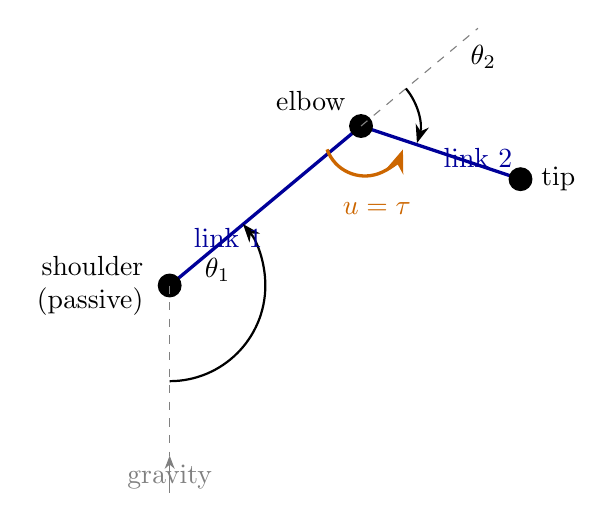
\begin{tikzpicture}[>=Stealth,scale=1.35]
  \coordinate (O) at (0,0);
  \coordinate (E) at (1.8,1.5);
  \coordinate (H) at (3.3,1.0);
  \draw[very thick,blue!60!black] (O)--(E);
  \draw[very thick,blue!60!black] (E)--(H);
  \fill (O) circle (3.2pt) node[left=6pt,align=right] {shoulder\\(passive)};
  \fill (E) circle (3.2pt) node[above left=3pt] {elbow};
  \fill (H) circle (3.2pt) node[right=4pt] {tip};
  \draw[dashed,gray] (O)--(0,-1.6);
  \draw[->,gray] (0,-1.95)--(0,-1.6);
  \node[gray] at (0,-1.8) {gravity};
  \draw[->,thick] (0,-0.9) arc[start angle=-90,end angle=40,radius=0.9];
  \node at (0.45,0.15) {$\theta_1$};
  \draw[dashed,gray] (E)--++(1.1,0.92);
  \draw[->,thick] (E) ++(40:0.55) arc[start angle=40,end angle=-17,radius=0.55];
  \node at (2.95,2.15) {$\theta_2$};
  \draw[->,very thick,orange!80!black] (E) ++(-0.32,-0.22)
       arc[start angle=200,end angle=340,radius=0.38];
  \node[orange!80!black] at (1.95,0.72) {$u=\tau$};
  \node[blue!60!black] at (0.55,0.45) {link 1};
  \node[blue!60!black] at (2.90,1.20) {link 2};
\end{tikzpicture}
\caption{Acrobot schematic.  The shoulder is not actuated; the only input is
the elbow torque $u=\tau$.  $\theta_1$ is measured from the downward vertical
and $\theta_2$ from the extension of link~1.  Because the shoulder has no
motor, the only way to move $\theta_1$ is through the inertial coupling
produced by the elbow motion.}
\label{fig:acrobot}
\end{figure}

\begin{intuition}[breakable=false,title={Why can a one-motor two-link robot still be controllable?}]
Imagine holding a chain by one end and moving it with your wrist.  The far
end is not directly actuated, but it moves because the links are coupled by
their mass and inertia.  The acrobot works the same way: the elbow torque
accelerates link~2, and the reaction on link~1 changes $\theta_1$.  This is
why the linearised pair $(A,B)$ can have rank~4 even though the shoulder has
no motor.  The coupling is not equally strong in all directions, however;
that is the meaning of ``weak controllability'' below.
\end{intuition}

\subsection{What was run}

The supplied notebook \texttt{Exp3'1-acrobot.ipynb} was run.  It
(i) simulates the response to a constant elbow torque, (ii) linearises the
system at $\x^\star$ and checks controllability, and (iii) closes an LQR loop
around $\x^\star$.  The numerical analysis in
\texttt{exp1\_analysis/exp1\_analysis.py} repeats the linearisation and runs
100-trial Monte-Carlo studies with and without the $\pm10$ N\,m actuator
limit.

\subsection{Linearisation and controllability}

At $\x^\star$,
\begin{equation}
\A=\begin{bmatrix}
0 & 0 & 1 & 0\\
0 & 0 & 0 & 1\\
12.629 & -12.693 & -0.172 & 0.3015\\
-14.749 & 29.612 & 0.3015 & -0.6033
\end{bmatrix},
\qquad
\B=\begin{bmatrix}0\\0\\-3.0147\\6.0332\end{bmatrix}.
\end{equation}
The open-loop eigenvalues are
\begin{equation}
\lambda(\A)=\{-6.492,\;-2.249,\;+2.231,\;+5.734\},
\end{equation}
so the upright position is unstable (two eigenvalues with positive real part).
The controllability matrix $\C=[\B,\A\B,\A^2\B,\A^3\B]$ has
\begin{equation}
\sigma(\C)=[511.7,\;123.1,\;0.0807,\;0.0715],
\qquad
\operatorname{rank}\C=4,
\qquad
\operatorname{cond}\C\approx 7.15\times10^3 .
\end{equation}

\textbf{Comment.}  The acrobot is underactuated (one actuator, two degrees of
freedom), yet the linearised system is completely controllable.  This is the
central lesson of Chapter~3: underactuation does not imply loss of
controllability; the passive joint is driven through the inertial coupling.
The very small last two singular values show, however, that some directions
are \emph{weakly} controllable.  The slow modes have input participation
factors of about $0.048$ compared with $3.6$ for the fast modes, so driving
them requires large inputs or long manoeuvres.

\subsection{LQR design and closed-loop behaviour}

With $Q=\operatorname{diag}(10,10,1,1)$ and $R=1$, the solved Riccati equation
gives the controller $u=D(\x-\x^\star)$ with
\begin{equation}
D=[\,278.44,\;112.29,\;119.72,\;56.83\,],
\end{equation}
and closed-loop poles
\begin{equation}
\lambda_{\mathrm{cl}}=\{-10.126,\;-4.238,\;-2.242\pm0.039j\}.
\end{equation}
All poles are in the left half-plane, hence the nonlinear closed loop is
locally exponentially stable at $\x^\star$.

\begin{figure}[htbp]
  \centering
  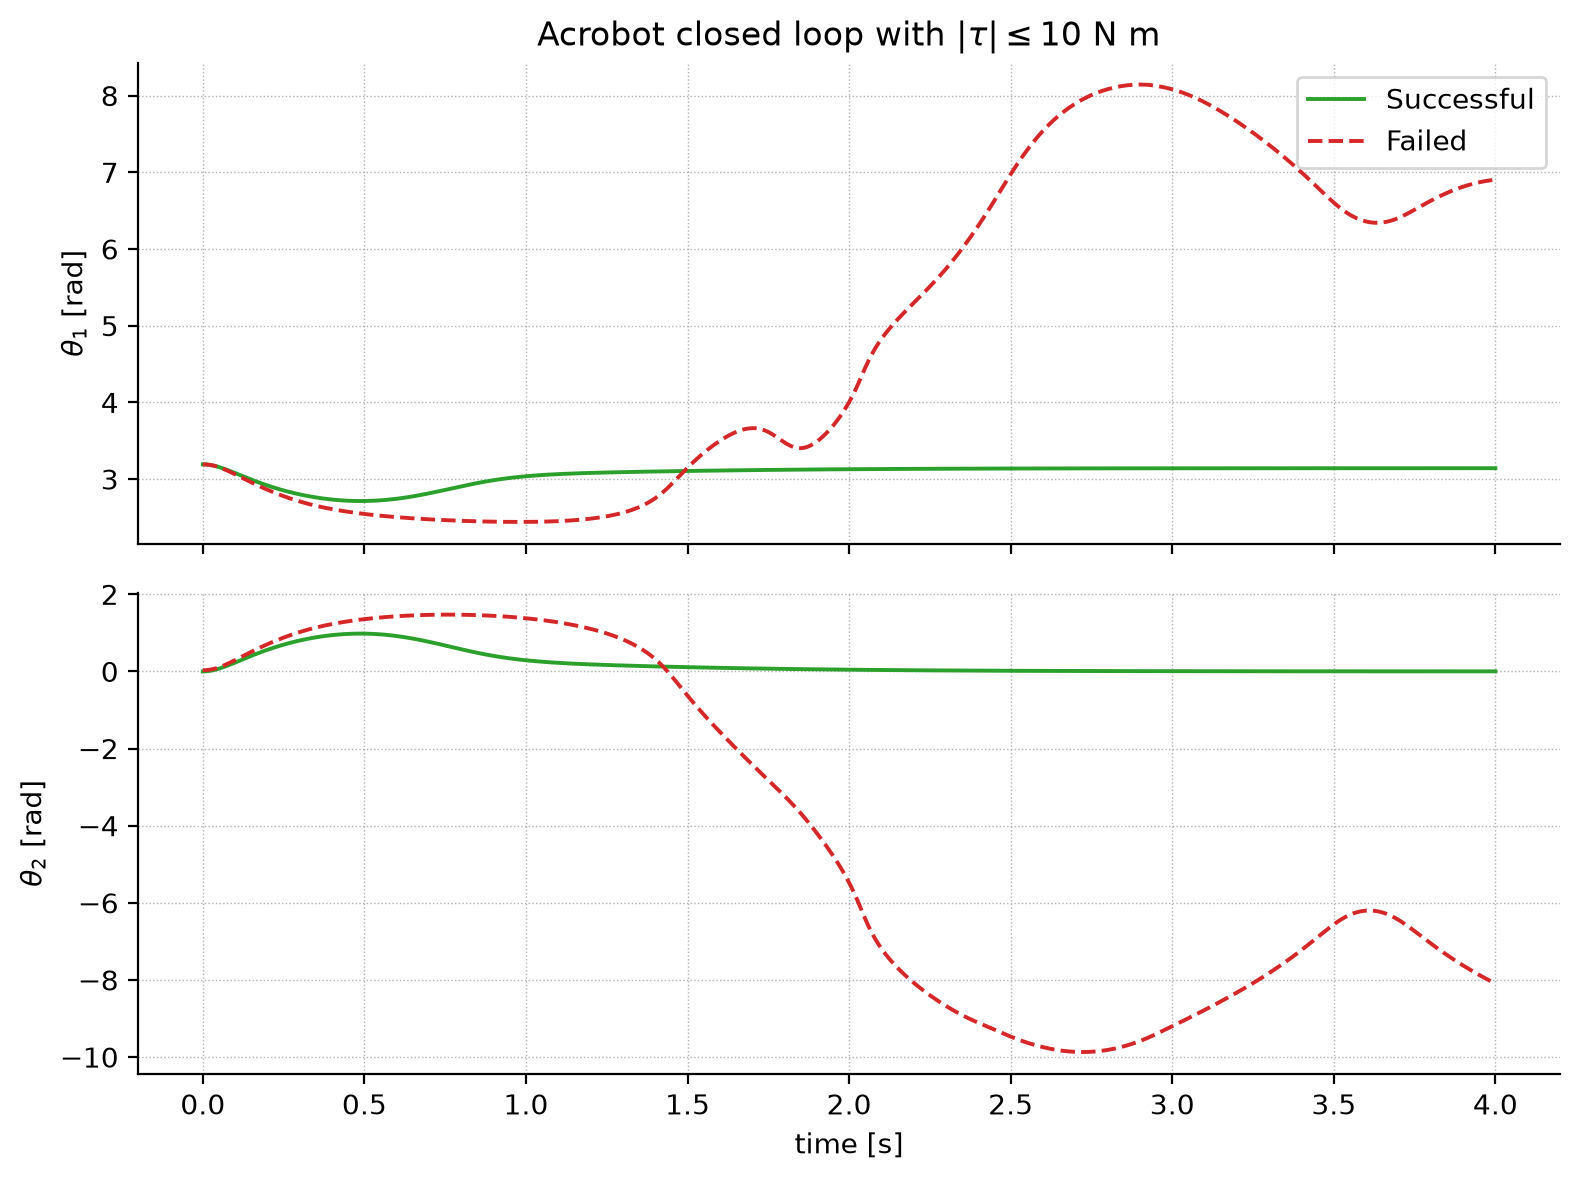
\includegraphics[width=0.78\textwidth]{acro_fig1_success_vs_failure.png}
  \caption{Acrobot: a successful (green) and a failed (red) closed-loop
  trajectory with the $\pm10$ N\,m saturation.  The successful trajectory
  shows the non-minimum-phase undershoot: the elbow first moves far away
  from zero before returning.}
  \label{fig:acro_success}
\end{figure}

The 100-trial Monte-Carlo study (initial state
$\x_0=\x^\star+0.05\,\mathcal N(0,I_4)$, horizon 4 s) gives:
\begin{center}
\begin{tabular}{lcc}
\toprule
Condition & Success rate & Peak torque (median) \\
\midrule
No saturation & 98\% & 11.2 N\,m \\
$|\tau|\le 10$ N\,m & 63\% & 11.2 N\,m \\
\bottomrule
\end{tabular}
\end{center}
The successful trials have a median peak angular deviation of 0.855 rad and a
median settling time of 1.63 s.

\textbf{Comment.}  Two effects explain the failures.  First, the linear LQR
guarantee is local; the nonlinear system has a finite basin of attraction.
Second, the saturated actuator turns the problem into a constrained nonlinear
one, for which the unconstrained LQR optimality no longer applies.  The
linearised system is also non-minimum phase: the right-half-plane zeros of
$u\to\theta_1$ are $\pm2.052$ and of $u\to\theta_2$ are $+2.283,-2.304$.
State feedback does not move zeros, so the closed loop must first move the
state away from the origin before returning; this is visible in
Fig.~\ref{fig:acro_success}.

\subsection{Sensitivity study}

\paragraph{Initial disturbance.}
\begin{center}
\begin{tabular}{lccccccc}
\toprule
$\delta$ & 0.005 & 0.02 & 0.05 & 0.075 & 0.10 & 0.15 & 0.20\\
\midrule
No saturation & 100\% & 100\% & 100\% & 98\% & 92\% & 82\% & 60\%\\
$|\tau|\le10$ N\,m & 100\% & 100\% & 70\% & 54\% & 42\% & 32\% & 18\%\\
\bottomrule
\end{tabular}
\end{center}

\begin{figure}[htbp]
  \centering
  \begin{subfigure}{0.48\textwidth}
    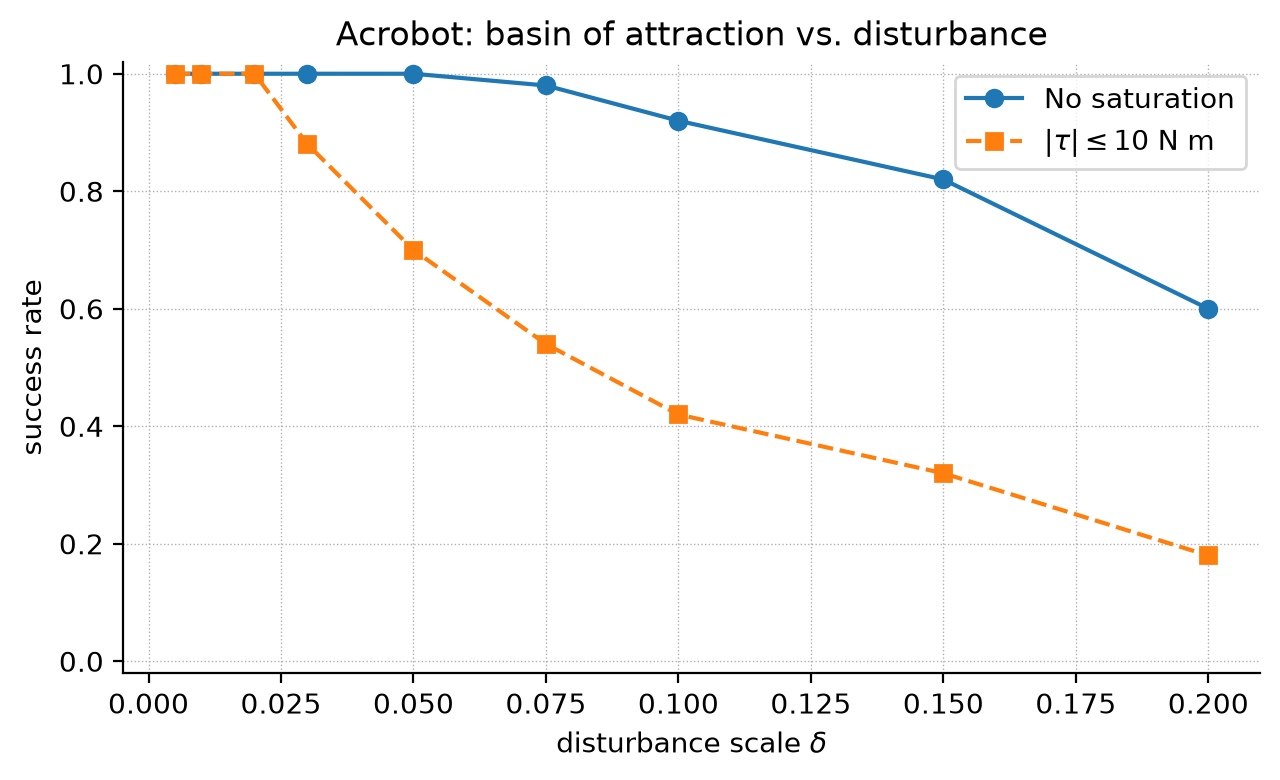
\includegraphics[width=\textwidth]{acro_fig2_delta_sweep.png}
    \caption{Success rate versus disturbance scale, with and without saturation.}
  \end{subfigure}\hfill
  \begin{subfigure}{0.48\textwidth}
    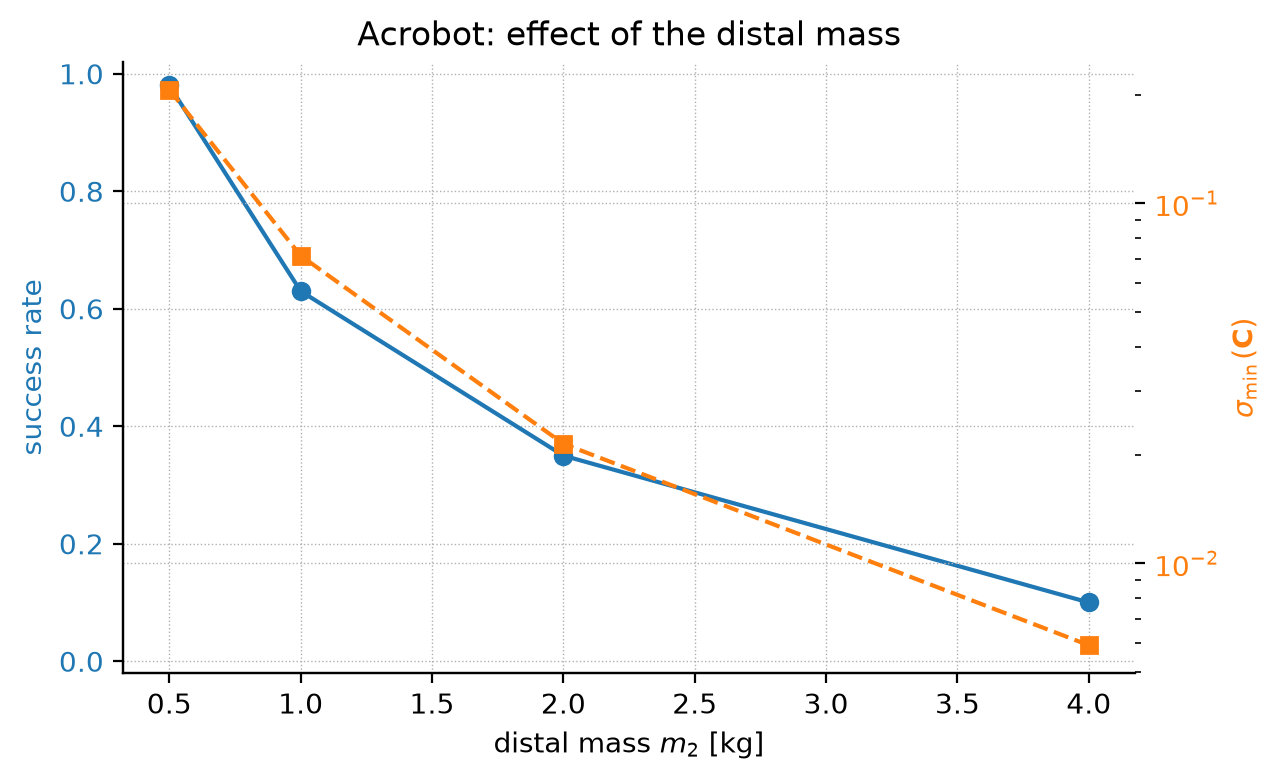
\includegraphics[width=\textwidth]{acro_fig3_m2_sweep.png}
    \caption{Effect of the distal mass $m_2$.}
  \end{subfigure}
  \caption{Acrobot sensitivity studies.  Saturation shrinks the basin of
  attraction substantially; increasing the distal mass makes the system much
  harder to control.}
\end{figure}

\paragraph{Distal mass $m_2$.}
\begin{center}
\begin{tabular}{lcccc}
\toprule
$m_2$ [kg] & 0.5 & 1.0 & 2.0 & 4.0\\
\midrule
$\sigma_{\min}(\C)$ & 0.207 & 0.0715 & 0.0215 & 0.0059\\
$\|D\|$ & 153.2 & 328.2 & 864.3 & 2655.7\\
Success rate & 98\% & 63\% & 35\% & 10\%\\
Median peak torque [N\,m] & 5.1 & 11.2 & 47.8 & 317.0\\
\bottomrule
\end{tabular}
\end{center}

\paragraph{Control weight $R$.}
\begin{center}
\begin{tabular}{lcccc}
\toprule
$R$ & 0.1 & 1 & 10 & 100\\
\midrule
$\|D\|$ & 577.1 & 328.2 & 289.7 & 285.5\\
Success rate & 65\% & 63\% & 62\% & 62\%\\
Median peak torque [N\,m] & 19.8 & 11.2 & 9.8 & 9.7\\
\bottomrule
\end{tabular}
\end{center}

\textbf{Comment.}  The success rate decreases monotonically with the
disturbance size, confirming the finite basin of attraction.  The distal mass
is the most sensitive physical parameter because it increases the effective
inertia and weakens the input leverage; the minimum singular value drops by a
factor of 35 and the success rate collapses from 98\% to 10\%.  Increasing $R$
reduces the peak torque only mildly: in the ``expensive control'' limit the
closed-loop poles tend to the mirrors of the stable open-loop poles and the
unstable poles, so the gain cannot go to zero for an unstable system.

%=====================================================================
\section{Example 3.2: Dynamics of the Cart-Pole System}
%=====================================================================

\subsection{Model and linearisation}

\begin{figure}[htbp]
\centering
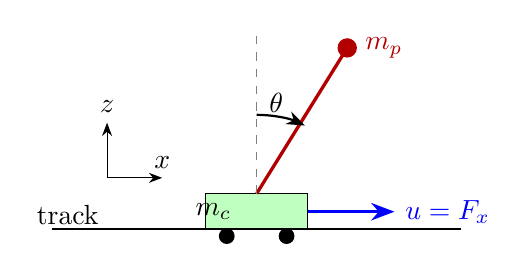
\begin{tikzpicture}[>=Stealth,scale=1.0]
  \draw[thick] (-2.6,0)--(2.6,0);
  \draw[fill=green!25,draw=black] (-0.65,0) rectangle (0.65,0.45);
  \fill[black] (-0.38,-0.09) circle (0.10);
  \fill[black] (0.38,-0.09) circle (0.10);
  \coordinate (P) at (0,0.45);
  \coordinate (T) at (1.15,2.30);
  \draw[very thick,red!70!black] (P)--(T);
  \fill[red!70!black] (T) circle (3.5pt) node[right=3pt] {$m_p$};
  \draw[dashed,gray] (P)--(0,2.55);
  \draw[->,thick] (0,1.45) arc[start angle=90,end angle=65,radius=1.45];
  \node at (0.25,1.60) {$\theta$};
  \draw[->,very thick,blue] (0.65,0.22)--(1.75,0.22) node[right] {$u=F_x$};
  \draw[->] (-1.9,0.65)--(-1.9,1.35) node[above] {$z$};
  \draw[->] (-1.9,0.65)--(-1.2,0.65) node[above] {$x$};
  \node at (-0.55,0.22) {$m_c$};
  \node at (-2.4,0.18) {track};
\end{tikzpicture}
\caption{Cart-pole schematic.  The cart of mass $m_c$ slides along $x$; the
pole of mass $m_p$ is attached by a passive hinge.  The only input is the
horizontal force $u=F_x$.  $\theta$ is measured from the upward vertical
($\theta=\pi$ is upright in the model used in this report).}
\label{fig:cartpole}
\end{figure}

\begin{intuition}[title={What the state and the input mean}]
$x$ is where the cart is, $\theta$ is how far the pole is from upright,
$\dot x$ and $\dot\theta$ are their velocities, and $u$ is the only force we
can apply.  There is no motor at the pole hinge, so the pole angle can only be
changed by moving the cart.  This is the whole difficulty of the cart-pole:
we must use one actuator to control two coordinates.
\end{intuition}

The cart-pole has state $\x=[x,\theta,\dot x,\dot\theta]^\top$ and input
$u=F_x$.  The model used by the notebook
(\texttt{underactuated/models/cartpole.urdf}) has $m_c=10$ kg, $m_p=1$ kg,
$l_c=0.5$ m and no joint damping.  The upright equilibrium is
$\x^\star=[0,\pi,0,0]^\top$.  Linearisation gives
\begin{equation}
\A=\begin{bmatrix}
0&0&1&0\\
0&0&0&1\\
0&0.981&0&0\\
0&21.582&0&0
\end{bmatrix},
\qquad
\B=\begin{bmatrix}0\\0\\0.1\\0.2\end{bmatrix}.
\end{equation}
The open-loop eigenvalues are $0,0,\pm4.6456$; the two zeros come from the cart
position integrator.  The controllability singular values are
\begin{equation}
\sigma(\C)=[4.326,\;4.326,\;0.0907,\;0.0907],
\qquad
\operatorname{cond}\C\approx47.7 .
\end{equation}

\textbf{Comment.}  The pair is controllable, but the two small singular values
correspond to the cart-position direction, which is only weakly controllable.
The transfer function from $u$ to $x$ has a right-half-plane zero at
$+4.43$: the cart must first move in the opposite direction to bring the pole
back.  This non-minimum-phase behaviour is visible as a cart undershoot of
about 0.3 m for a 0.1 disturbance.

\begin{pitfall}[title={What a right-half-plane zero really means}]
A zero at $+4.43$ does not mean that the system is unstable.  It means that
the cart's response to a force starts in the \emph{opposite} direction.
Physically: to bring the pole back to the left, the cart first accelerates to
the right so that the pole starts falling left; then the cart reverses to
catch it.  The net initial displacement is therefore opposite to the final
one.  This ``undershoot'' is not a controller bug: state feedback cannot move
a zero, so LQR keeps it.  It also explains why the cart moves about 0.3 m in
the wrong direction for a 0.1 disturbance, and why aggressive saturation can
destroy the recovery.
\end{pitfall}

\subsection{LQR results and sensitivity}

With $Q=\operatorname{diag}(10,10,1,1)$ and $R=1$, the gain is
\begin{equation}
D=[\,3.1623,\;-254.3925,\;9.7692,\;-55.1774\,],
\qquad u=D(\x-\x^\star),
\end{equation}
with closed-loop poles
\begin{equation}
-4.7206,\quad -4.5739,\quad -0.3820\pm0.3761j.
\end{equation}
The two fast poles bring the pole back; the slow complex pair is the cart
returning to the origin (time constant $\approx2.6$ s).  Over a 5 s horizon the
cart often has not fully returned even when the pole is balanced.

\begin{figure}[htbp]
  \centering
  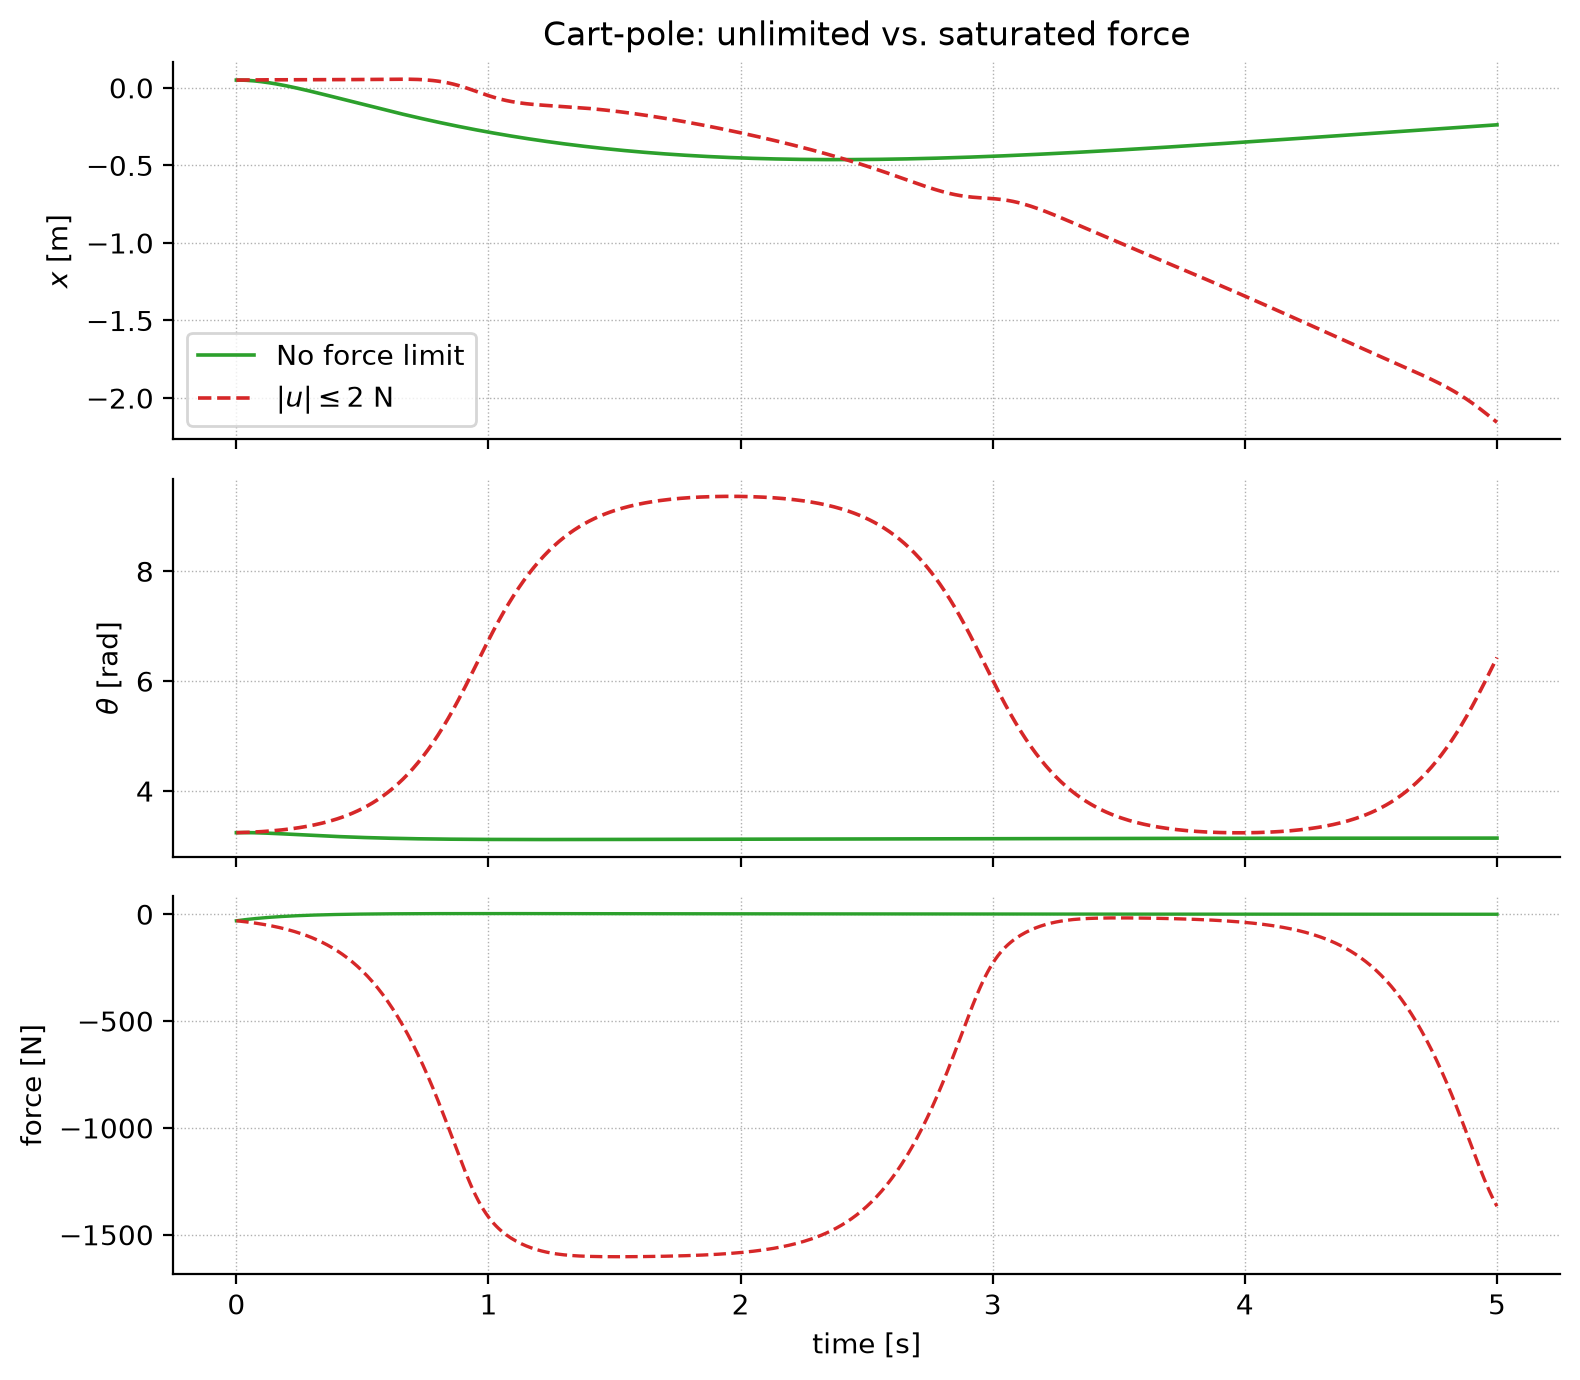
\includegraphics[width=0.82\textwidth]{cp_fig1_success_vs_limit.png}
  \caption{Cart-pole: the same initial condition without a force limit
  (green) and with a $\pm2$ N limit (red).  The unlimited controller balances
  the pole, whereas the saturated one loses it.}
  \label{fig:cp_limit}
\end{figure}

The 100-trial study with $\x_0=\x^\star+0.1\,\mathcal N(0,I_4)$ gives:
\begin{center}
\begin{tabular}{lccc}
\toprule
Condition & Pole balanced & Full state & Peak force (median) \\
\midrule
No limit & 100\% & 98\% & 17.2 N \\
$|u|\le20$ N & 90\% & 82\% & -- \\
$|u|\le5$ N & 36\% & 33\% & -- \\
\bottomrule
\end{tabular}
\end{center}

\begin{figure}[htbp]
  \centering
  \begin{subfigure}{0.48\textwidth}
    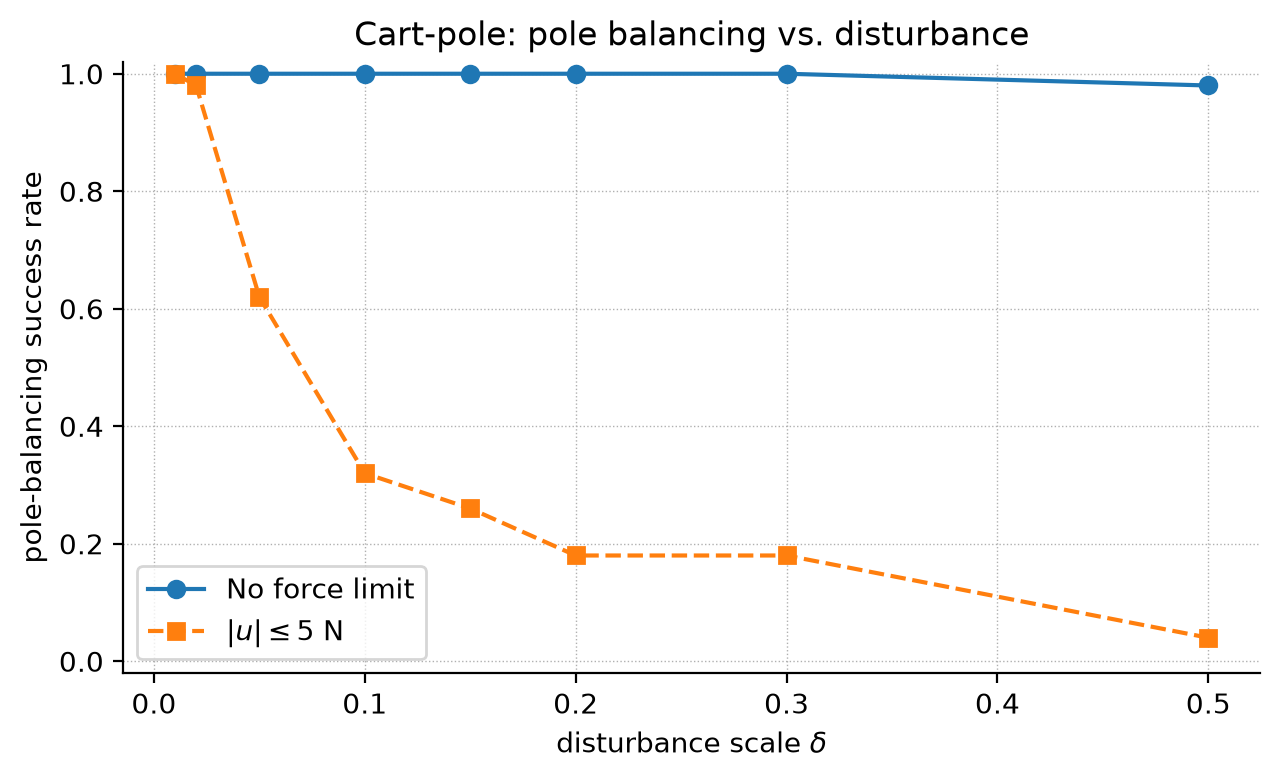
\includegraphics[width=\textwidth]{cp_fig2_delta_sweep.png}
    \caption{Disturbance-size sweep.}
  \end{subfigure}\hfill
  \begin{subfigure}{0.48\textwidth}
    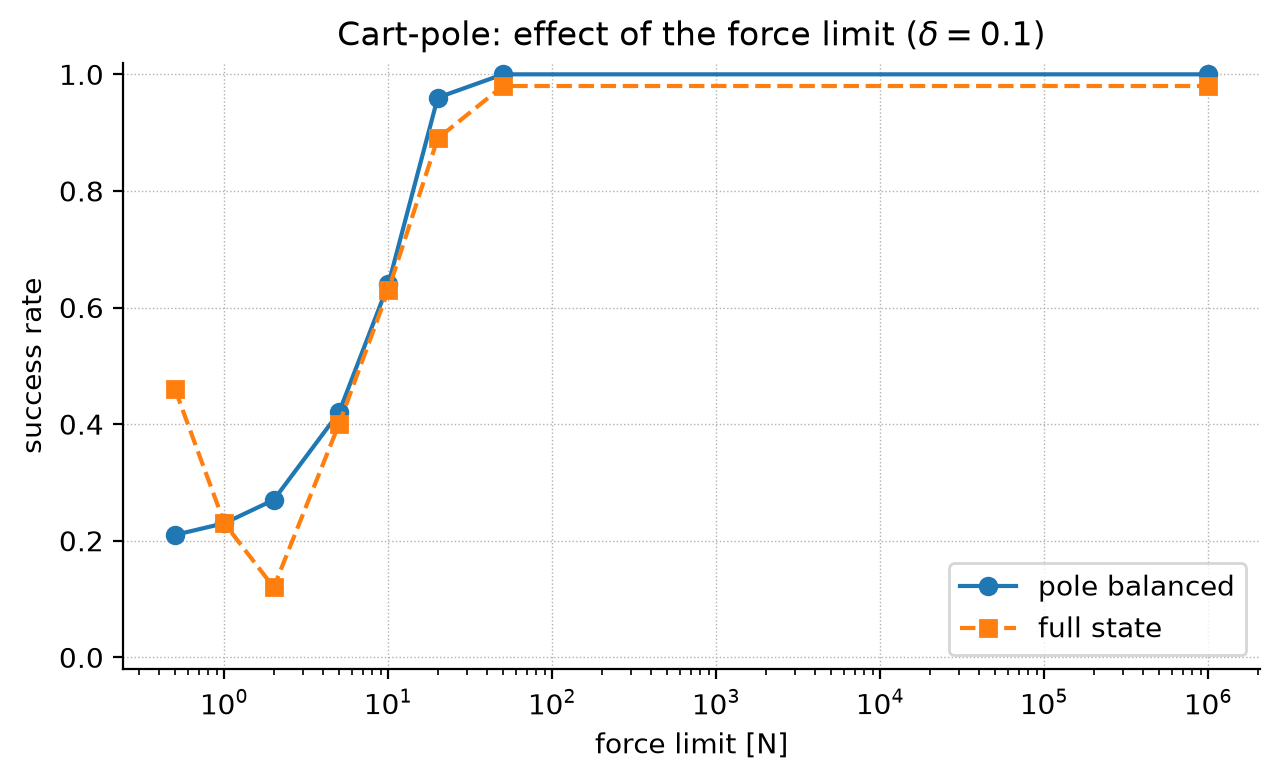
\includegraphics[width=\textwidth]{cp_fig3_force_limit.png}
    \caption{Effect of the force limit at $\delta=0.1$.}
  \end{subfigure}
  \caption{Cart-pole sensitivity: the pole itself is robust without
  saturation, but a realistic force limit quickly reduces the basin of
  attraction.}
\end{figure}

\begin{figure}[htbp]
  \centering
  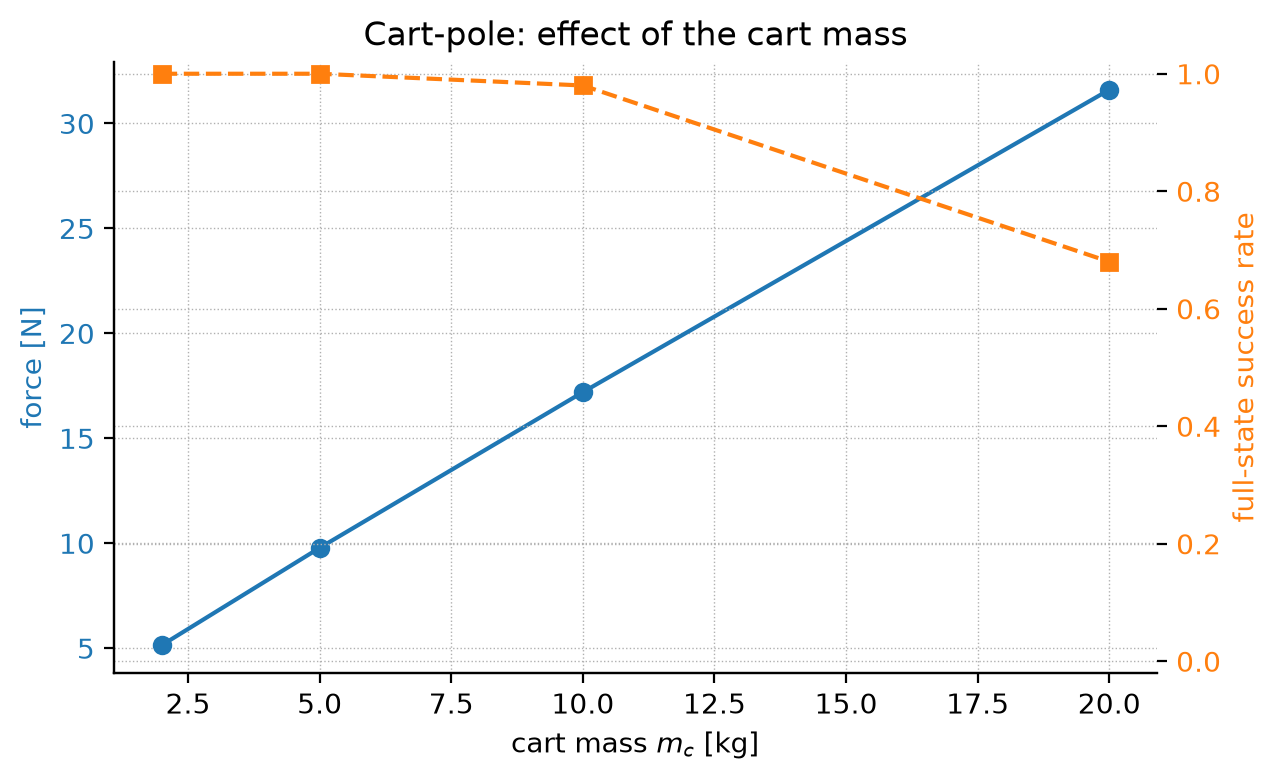
\includegraphics[width=0.72\textwidth]{cp_fig4_physical.png}
  \caption{Effect of the cart mass $m_c$.  A heavier cart requires more force
  and slows down the cart-return mode.}
\end{figure}

\textbf{Comment.}  The original notebook has no force saturation, so the pole
almost always balances.  The real constraint is the actuator: the median peak
force is 17.2 N and the 90th percentile is 40 N.  When the limit is reduced to
5 N, saturation destroys the non-minimum-phase undershoot and the pole falls.
The cart mass is the dominant physical parameter: from 2 to 20 kg the required
force grows from about 5 N to 32 N and the full-state success rate falls from
100\% to 68\%, while the pole itself remains balanceable without saturation.
Increasing $R$ saves force but makes the slow cart mode slower; for $R=100$
the slow pole is about $-0.12$, so the cart cannot return within 5 s.

%=====================================================================
\section{Example 3.5: LQR for the Acrobot and Cart-Pole}
%=====================================================================

\subsection{Theory and design}

For $\dot\x=\A\x+\B u$ and the cost
\begin{equation}
J=\int_0^\infty \left(\x^\top\Q\x+u^\top\R u\right)dt,
\end{equation}
the optimal state feedback is $u=-\R^{-1}\B^\top P\x$ with $P$ solving the
continuous-time algebraic Riccati equation
\begin{equation}
\A^\top P+P\A-P\B\R^{-1}\B^\top P+\Q=0.
\end{equation}
If the linearised pair is stabilisable, LQR returns a stabilising gain for any
$\Q\succeq0$, $\R\succ0$.  The closed-loop eigenvalues determine local
exponential stability of the nonlinear system; they say nothing about the
size of the basin of attraction or about input saturation.

\begin{figure}[htbp]
\centering
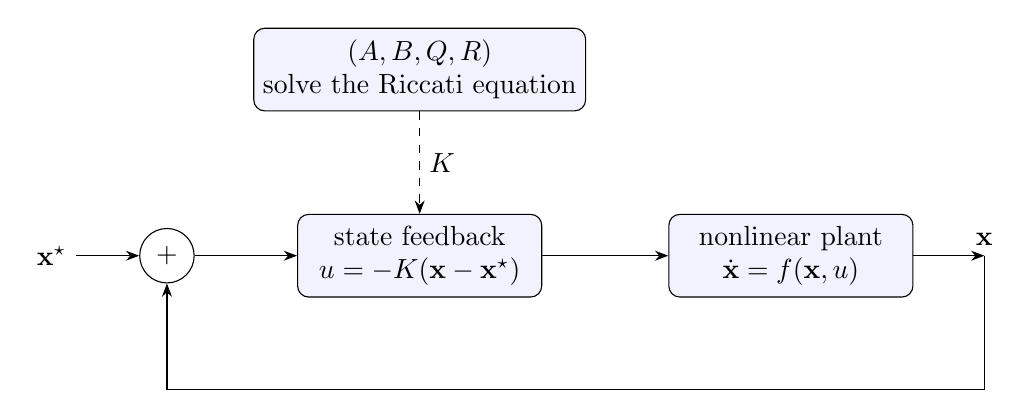
\begin{tikzpicture}[>=Stealth,node distance=1.5cm,
  box/.style={draw,rounded corners,align=center,fill=blue!5,
              minimum width=3.1cm,minimum height=1.05cm}]
  \node[box] (design) {$(A,B,Q,R)$\\ solve the Riccati equation};
  \node[box,below=1.3cm of design] (ctrl) {state feedback\\ $u=-K(\x-\x^\star)$};
  \node[box,right=1.6cm of ctrl] (plant) {nonlinear plant\\ $\dot\x=f(\x,u)$};
  \node[circle,draw,left=1.3cm of ctrl] (sum) {$+$};
  \node[left=0.8cm of sum] (ref) {$\x^\star$};
  \draw[->] (ref)--(sum);
  \draw[->] (sum)--(ctrl);
  \draw[->] (ctrl)--(plant);
  \draw[->] (plant.east)--++(0.9,0) node[above] {$\x$};
  \draw[->] (plant.east)++(0.9,0)--++(0,-1.7)-|(sum.south);
  \draw[->,dashed] (design)--(ctrl) node[midway,right] {$K$};
\end{tikzpicture}
\caption{LQR at a glance.  The design block solves the algebraic Riccati
equation once, offline.  The online controller is just a linear state
feedback, so it is cheap to run.  The nonlinear simulation is what tells us
how far from $\x^\star$ the linear guarantee remains useful.}
\label{fig:lqr_block}
\end{figure}

\begin{intuition}[title={Reading $Q$ and $R$}]
Think of the cost as a negotiation between two goals.  $Q$ says ``keep the
state close to the equilibrium''; $R$ says ``do not use too much actuator
effort''.  Increasing $Q$ (or decreasing $R$) makes the controller more
aggressive: it corrects faster but uses larger inputs.  Increasing $R$ makes
it gentler: smaller inputs, slower response, and often a larger steady-state
error under a disturbance.  The Riccati equation finds the best compromise
for the \emph{linear} model; it knows nothing about saturation, friction or
the size of the nonlinear basin.  That is why the simulations in this report
are essential.
\end{intuition}

\subsection{Comparison of the two systems}

\begin{table}[htbp]
\centering
\caption{Linearisation and LQR comparison (Drake default parameters).}
\begin{tabular}{lcc}
\toprule
 & Acrobot & Cart-pole \\
\midrule
Controllability rank & 4 & 4 \\
Condition number of $\C$ & $7.15\times10^3$ & 47.7 \\
Right-half-plane zeros & $+2.05$, $+2.28$ & $+4.43$ \\
Gain $D$ ($u=D(\x-\x^\star)$) & $[278.4,112.3,119.7,56.8]$ & $[3.16,-254.4,9.77,-55.2]$ \\
Closed-loop poles & $-10.13,-4.24,-2.24\pm0.04j$ & $-4.72,-4.57,-0.38\pm0.38j$ \\
\bottomrule
\end{tabular}
\end{table}

\begin{figure}[htbp]
  \centering
  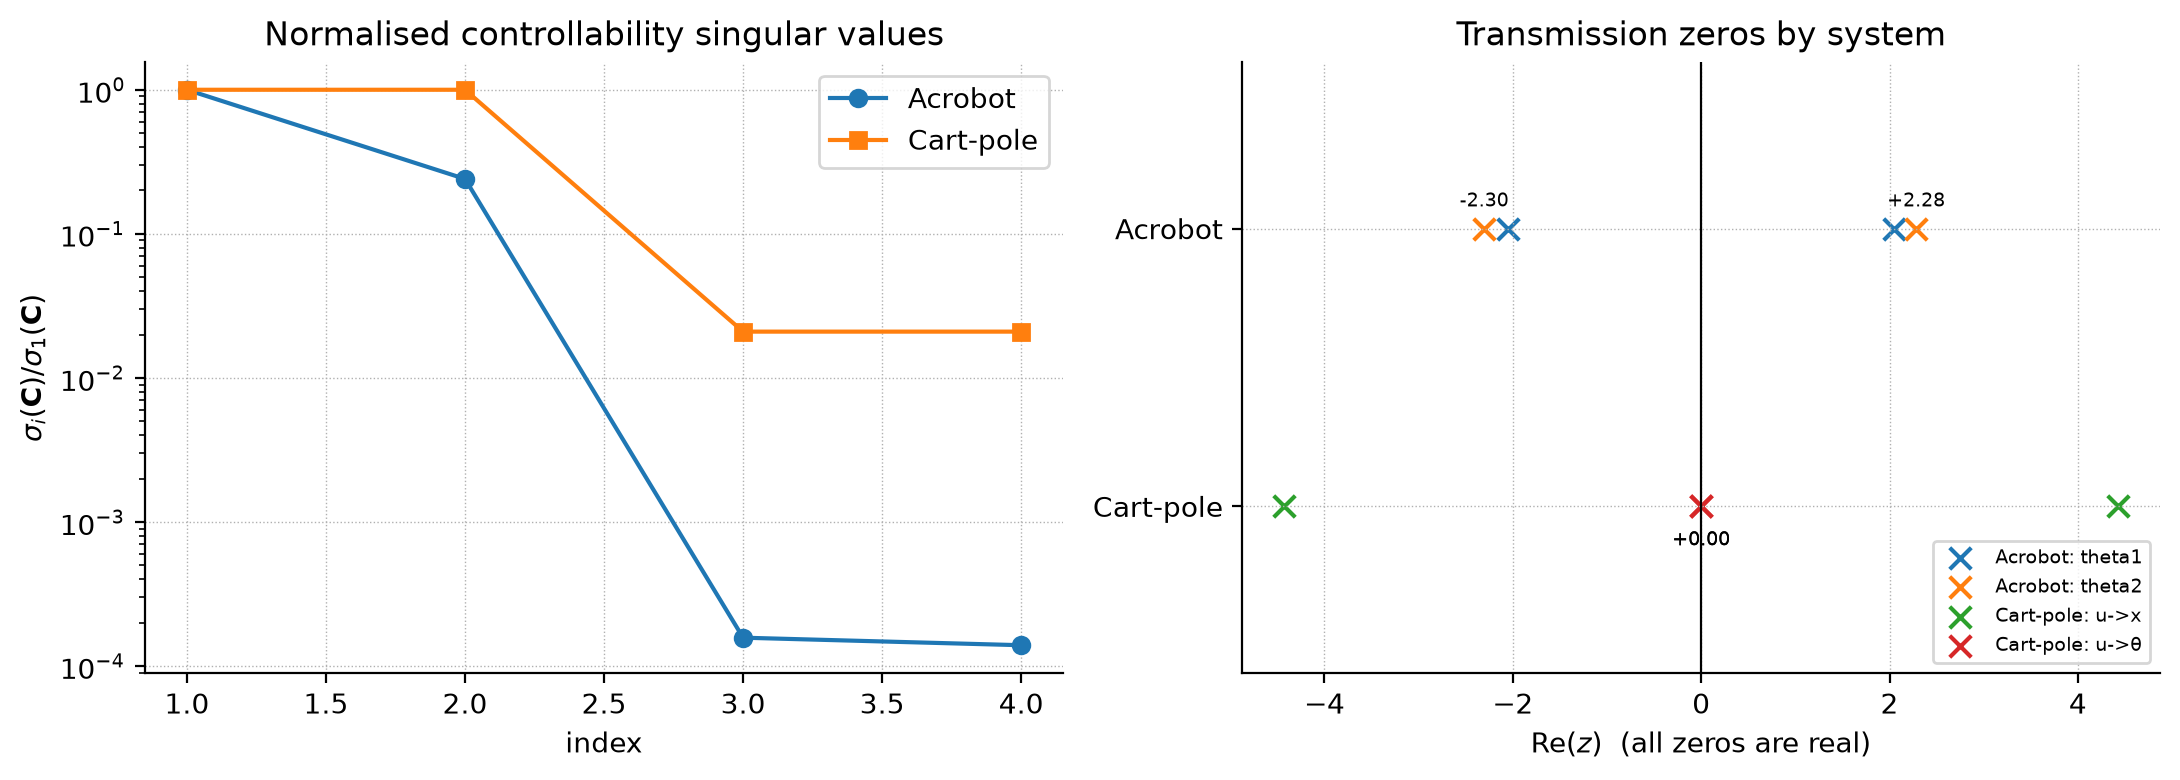
\includegraphics[width=0.88\textwidth]{lqr_fig1_linear.png}
  \caption{Normalised controllability singular values and right-half-plane
  zeros.  Both systems are controllable, but the acrobot is much more weakly
  controllable; both are non-minimum phase.}
\end{figure}

\textbf{Comment.}  Both systems are underactuated and both are controllable.
The acrobot is much more weakly controllable (condition number about 150 times
larger), because the passive shoulder is driven only through the elbow
coupling.  The cart-pole has two zero eigenvalues from the cart integrator,
which produce a slow closed-loop mode.  Both have right-half-plane zeros, so
the closed loop necessarily exhibits undershoot.

\subsection{Saturation and sensitivity}

\begin{table}[htbp]
\centering
\caption{Baseline success rates for 100 random disturbances.}
\begin{tabular}{llcc}
\toprule
System & Input constraint & Success & Peak control \\
\midrule
Acrobot & none & 98\% & median 11.2 N\,m \\
Acrobot & $|\tau|\le10$ N\,m & 63\% & -- \\
Cart-pole & none & 100\% (pole), 99\% (full) & median 18.4 N \\
Cart-pole & $|u|\le20$ N & 90\% (pole), 82\% (full) & -- \\
Cart-pole & $|u|\le5$ N & 36\% (pole), 33\% (full) & -- \\
\bottomrule
\end{tabular}
\end{table}

\begin{figure}[htbp]
  \centering
  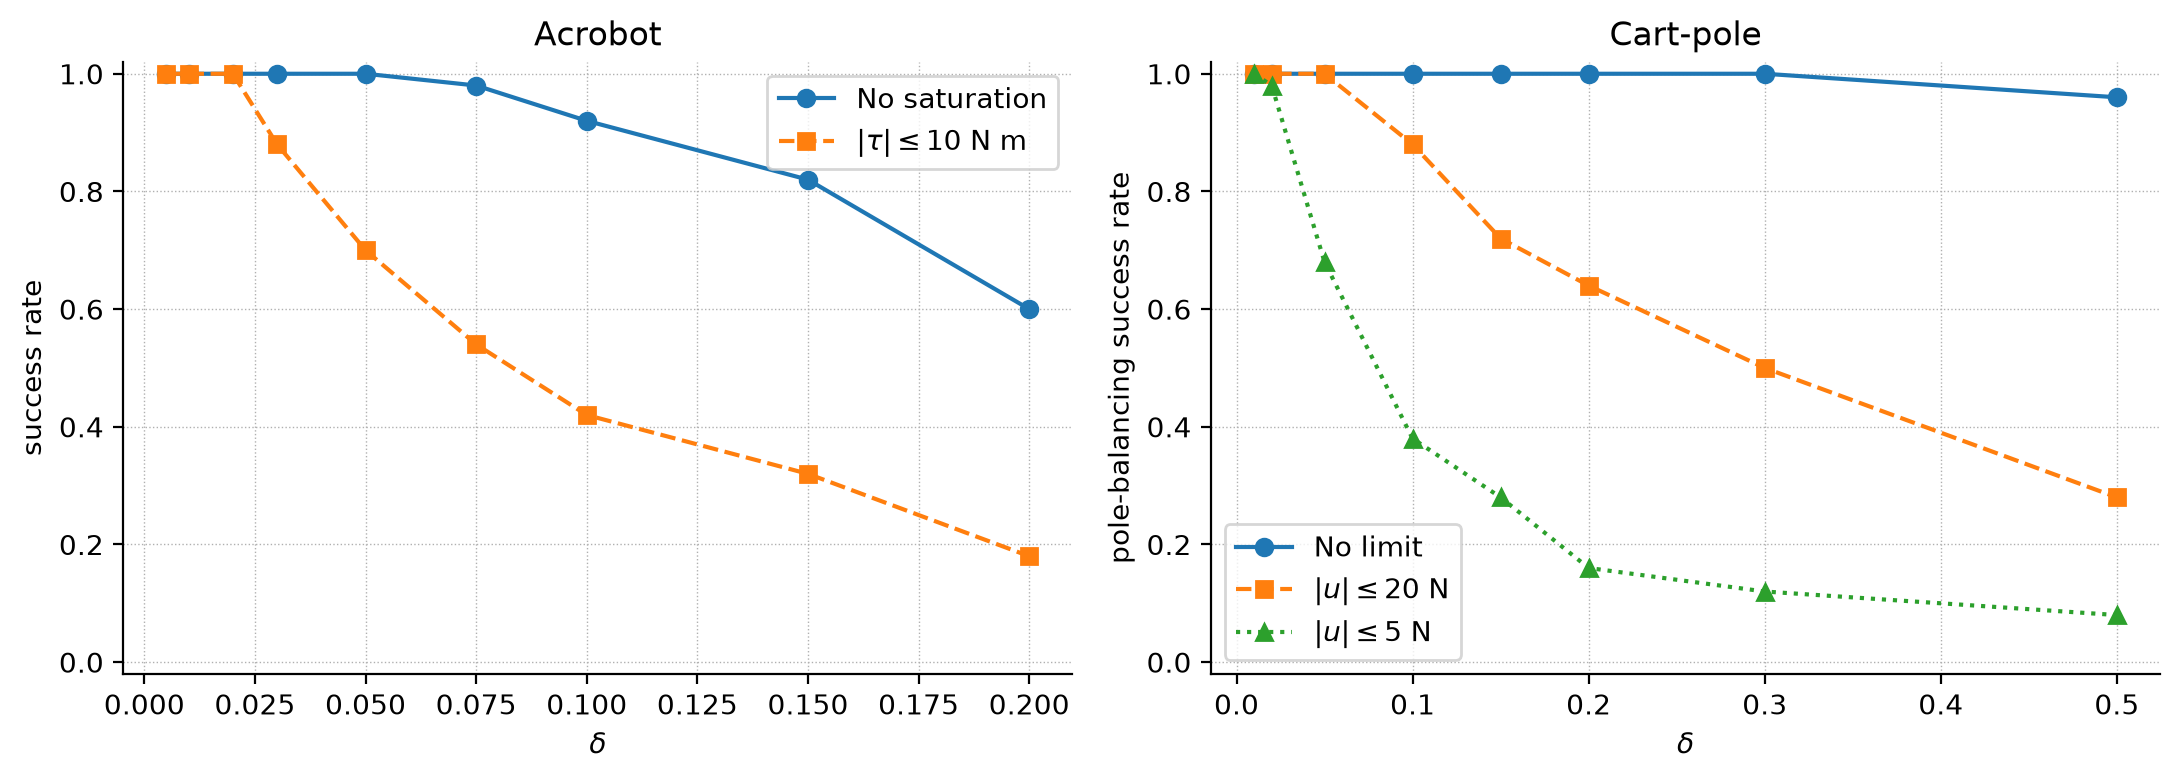
\includegraphics[width=0.9\textwidth]{lqr_fig2_robustness.png}
  \caption{Success rate versus disturbance scale for the acrobot with and
  without torque saturation (left) and the cart-pole with different force
  limits (right).}
\end{figure}

\begin{figure}[htbp]
  \centering
  \begin{subfigure}{0.48\textwidth}
    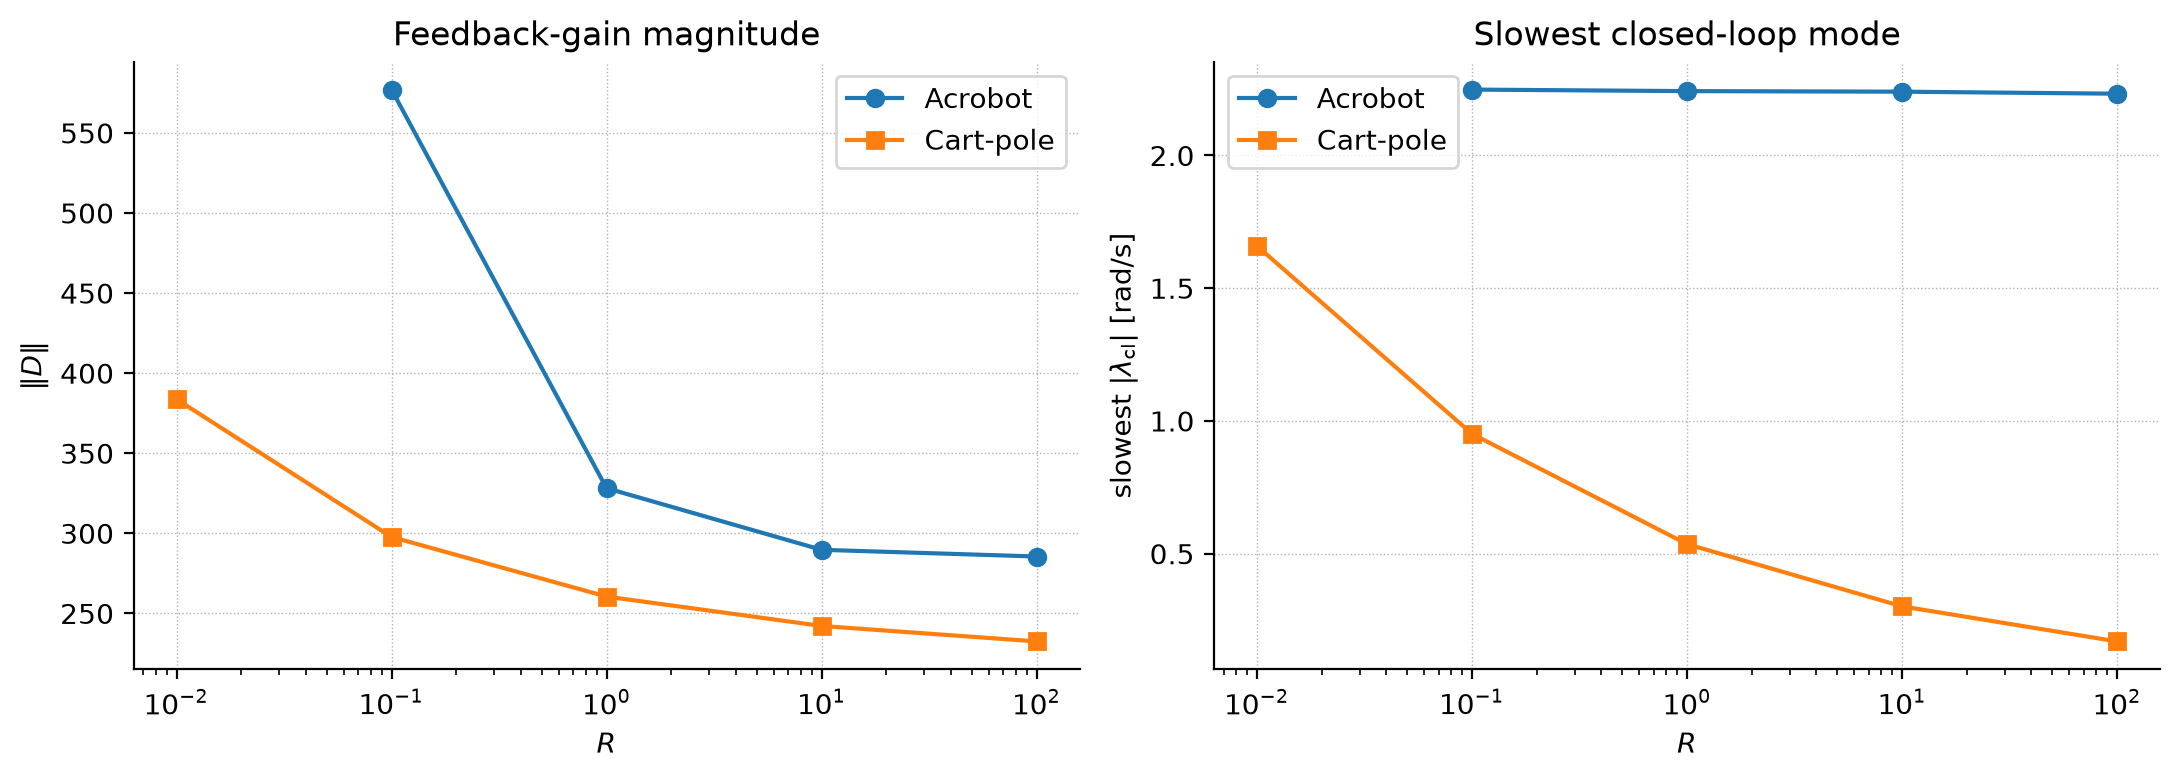
\includegraphics[width=\textwidth]{lqr_fig3_weights.png}
    \caption{Effect of $R$ on the gain and the slow pole.}
  \end{subfigure}\hfill
  \begin{subfigure}{0.48\textwidth}
    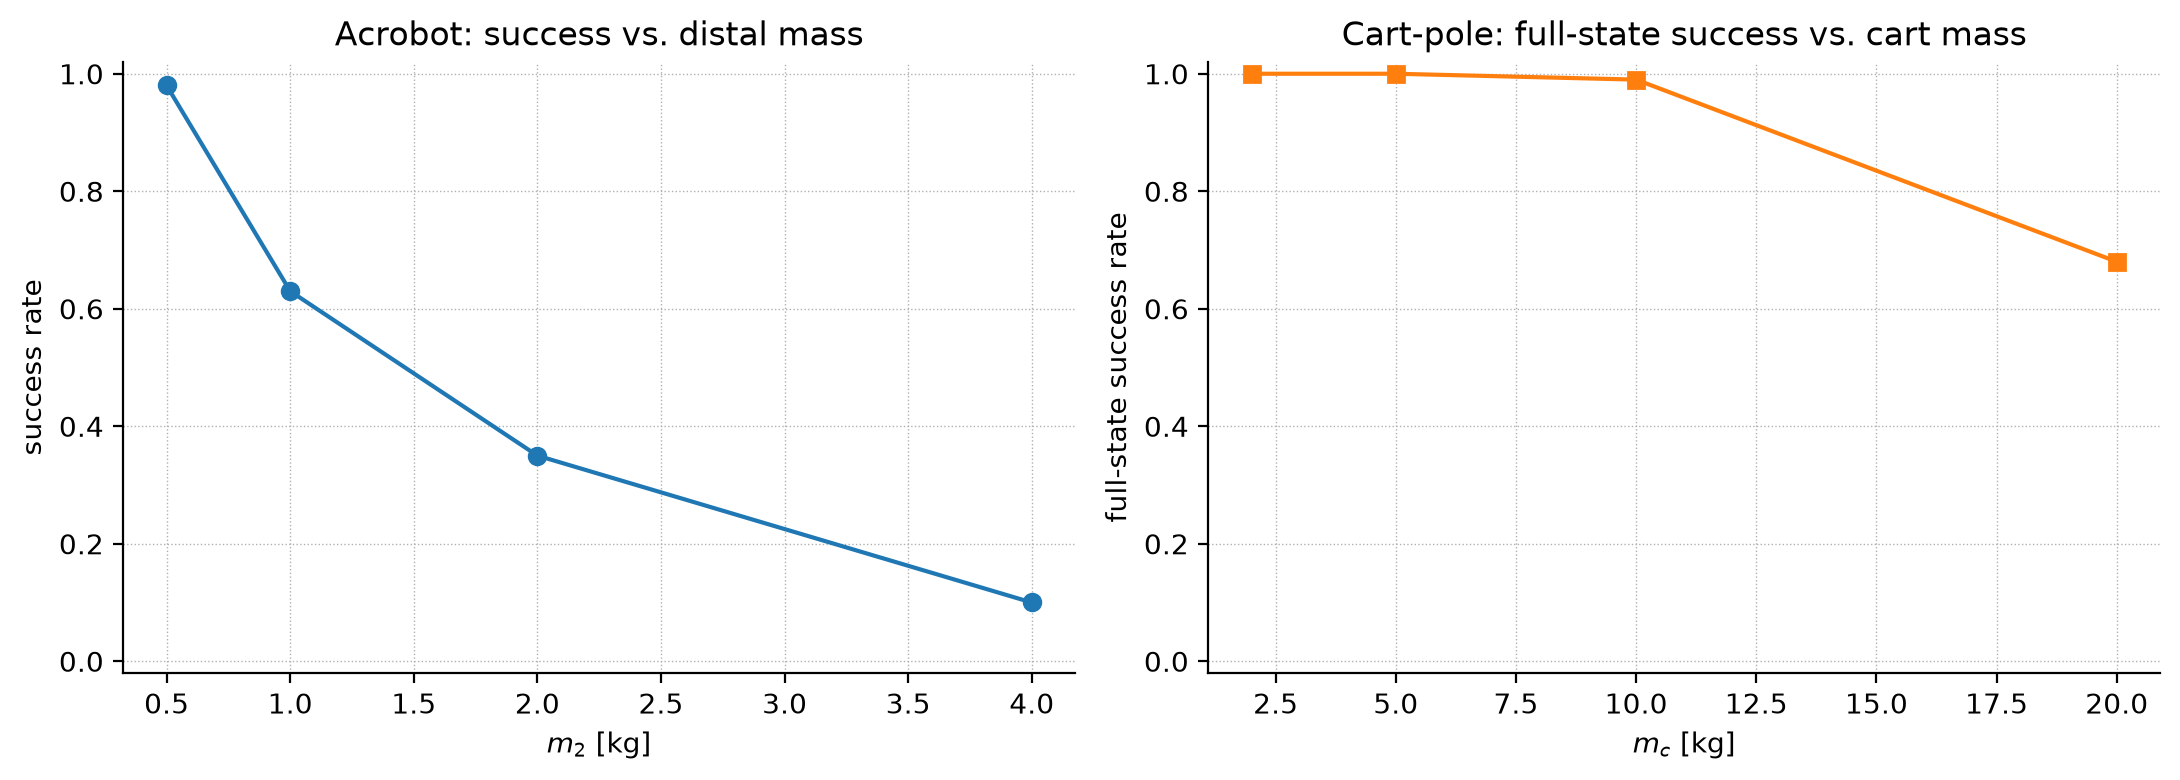
\includegraphics[width=\textwidth]{lqr_fig4_physical.png}
    \caption{Physical-parameter sensitivity.}
  \end{subfigure}
  \caption{Weight and parameter sensitivity.  For the cart-pole, increasing
  $R$ slows the cart-return mode; for the acrobot, the distal mass is the
  critical parameter.}
\end{figure}

\textbf{Comment.}  The acrobot needs a finite minimum torque even in the
``expensive control'' limit, because its linearisation has unstable poles.
The cart-pole's slow pole moves from $1.66$ to $0.17$ rad/s as $R$ grows from
0.01 to 100, so the full-state success rate falls from 100\% to 27\% even
though the pole remains balanced.  The physical-parameter studies show two
different failure modes: the acrobot becomes genuinely uncontrollable in
practice when $m_2$ is large, whereas the cart-pole mainly needs more force
and a longer time for the cart to return.

%=====================================================================
\section{Example 3.6: LQR for Quadrotors}
%=====================================================================

\begin{figure}[htbp]
\centering
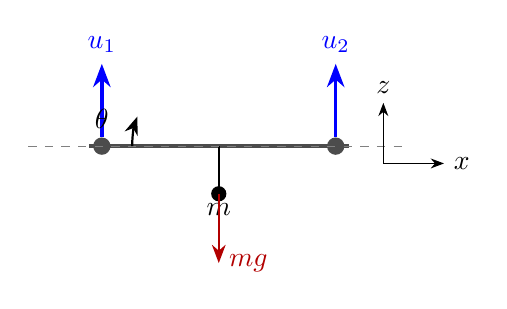
\begin{tikzpicture}[>=Stealth,scale=1.1]
  \draw[very thick,black!70] (-1.5,0)--(1.5,0);
  \fill[black!70] (-1.35,0) circle (0.10);
  \fill[black!70] (1.35,0) circle (0.10);
  \draw[thick] (0,0)--(0,-0.55);
  \fill (0,-0.55) circle (2.5pt) node[below] {$m$};
  \draw[->,very thick,blue] (-1.35,0.10)--(-1.35,0.95) node[above] {$u_1$};
  \draw[->,very thick,blue] (1.35,0.10)--(1.35,0.95) node[above] {$u_2$};
  \draw[->,thick,red!70!black] (0,-0.55)--(0,-1.35) node[right] {$mg$};
  \draw[dashed,gray] (-2.2,0)--(2.2,0);
  \draw[->,thick] (-1.0,0) arc[start angle=180,end angle=160,radius=1.0];
  \node at (-1.35,0.32) {$\theta$};
  \draw[->] (1.9,-0.2)--(2.6,-0.2) node[right] {$x$};
  \draw[->] (1.9,-0.2)--(1.9,0.5) node[above] {$z$};
\end{tikzpicture}
\caption{Planar quadrotor schematic.  The two propeller thrusts are the only
inputs.  At hover, $u_1+u_2=mg$ and $\theta=0$.  The vehicle can translate by
tilting and then using the horizontal component of the total thrust.}
\label{fig:planar_quad}
\end{figure}

\subsection{Planar quadrotor}

The planar quadrotor has state
\begin{equation}
\x=[x,z,\theta,\dot x,\dot z,\dot\theta]^\top
\end{equation}
and inputs $u=[u_1,u_2]^\top$ (two propeller thrusts).  With mass $m$, arm
length $l$, inertia $I$ and gravity $g$, the dynamics are
\begin{align}
\ddot x &= \frac{1}{m}\left(w_x-(u_1+u_2)\sin\theta\right),\\
\ddot z &= \frac{1}{m}\left(w_y+(u_1+u_2)\cos\theta\right)-g,\\
\ddot\theta &= \frac{l}{I}(u_1-u_2),
\end{align}
where $w_x,w_y$ denote a disturbance (wind) force.  The model parameters are
$m=0.486$ kg, $l=0.25$ m and $I=0.00383$ kg\,m$^2$.  The hover equilibrium is
$\theta=0$, $u_1=u_2=mg/2$.  The supplied planar notebook \texttt{Exp3'6-planar-quadrotor.ipynb}
was run and the quantitative studies below were produced by
\texttt{quadrotor\_analysis.py}.  The example uses
\begin{equation}
\Q=\operatorname{diag}\!\left(10,10,10,1,1,\frac{l}{2\pi}\right),
\qquad
\R=\begin{bmatrix}0.1&0.05\\0.05&0.1\end{bmatrix}.
\end{equation}

\begin{intuition}[breakable=false,title={Why LQR ``works out of the box'' for a quadrotor}]
The 3D quadrotor has four propeller inputs but six degrees of freedom, so it
is underactuated: it cannot independently command position and attitude at
the same instant.  Nevertheless, the hover equilibrium is \emph{stabilisable}.
The linearisation is taken around a point where the total thrust balances
gravity ($u_i=mg/4$), not around zero thrust; this is the key detail.  The
LQR then coordinates the four thrusts to correct roll/pitch, which produces
horizontal acceleration, and finally brings the vehicle back to the hover
position.  There is no integral action, so a constant wind causes a
steady-state position offset; this is visible in the sensitivity study.
\end{intuition}

\paragraph{Baseline.}  The resulting LQR has closed-loop poles
\begin{equation}
-80.75,\;-15.86,\;-6.59,\;-3.60,\;-2.72\pm1.61j.
\end{equation}
From the initial condition $(0,0,0.2,0,0,0)$ the controller settles in about
$0.06$ s with a peak thrust of $5.17$ N.  Ten random initial conditions with
standard deviation $0.1$ all recover, i.e.\ a $100\%$ success rate.

\begin{figure}[htbp]
  \centering
  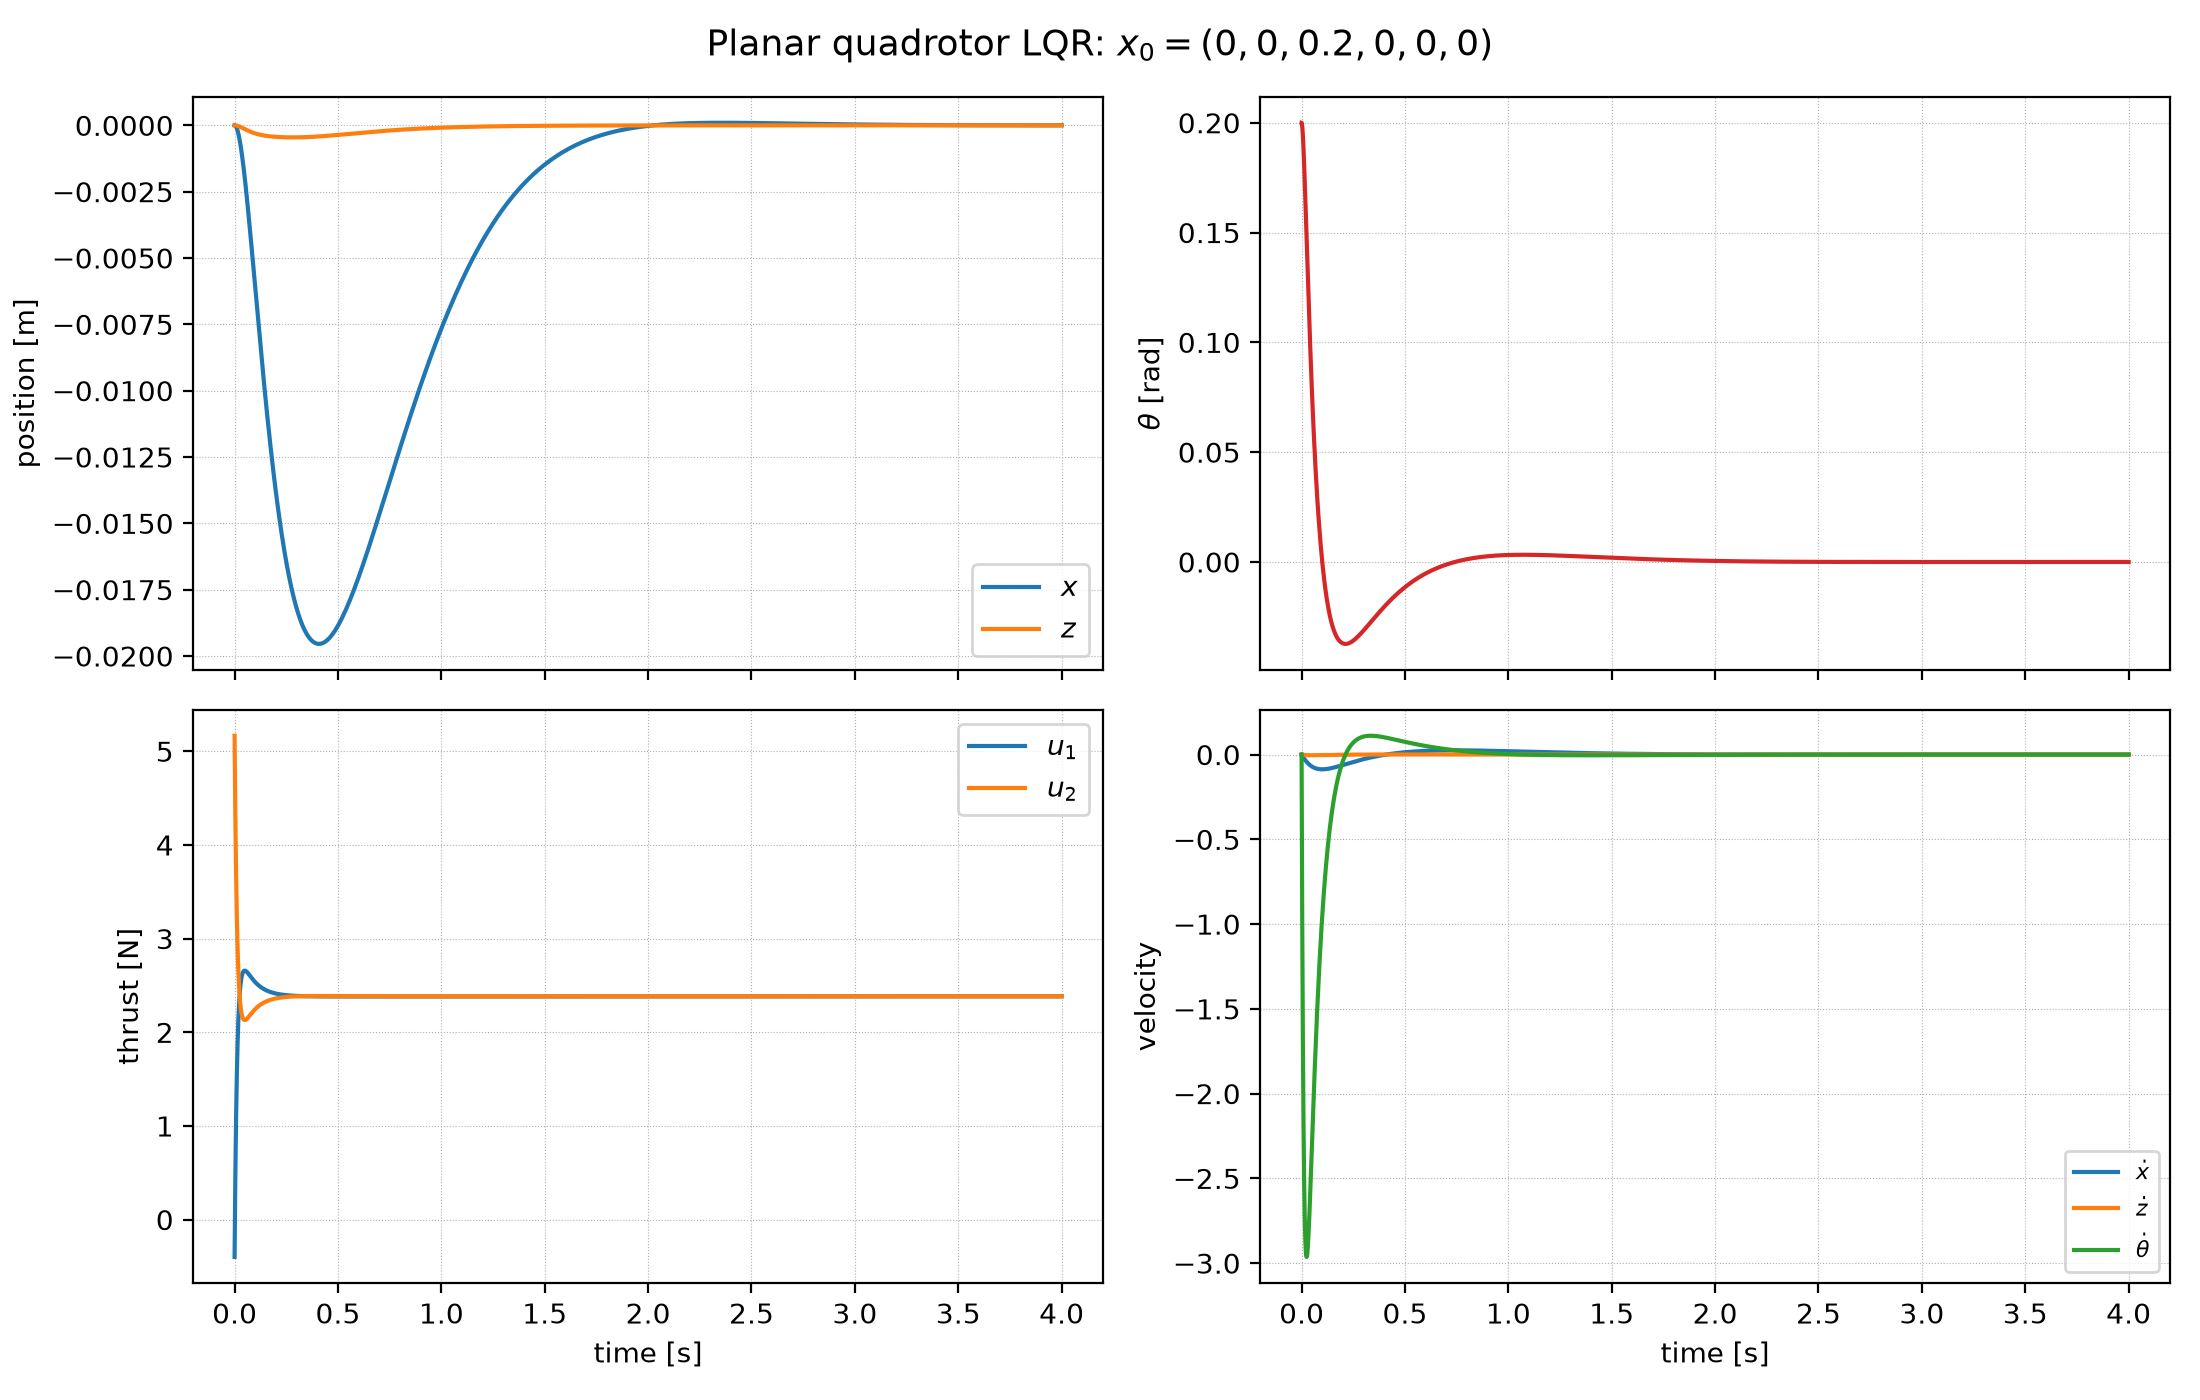
\includegraphics[width=0.8\textwidth]{quad_fig1_planar_baseline.png}
  \caption{Planar quadrotor LQR from $(0,0,0.2,0,0,0)$: position, attitude,
  velocities and the two thrusts.  The initial tilt produces a downward
  excursion before the vehicle returns to hover.}
\end{figure}

\paragraph{Sensitivity.}  Four studies are shown in
Fig.~\ref{fig:planar_sens}:
\begin{enumerate}[leftmargin=1.4em]
  \item increasing the position/attitude weight in $\Q$ makes the response
        faster but increases the peak thrust;
  \item increasing $\R$ makes the controller less aggressive: the peak thrust
        decreases while the settling time increases;
  \item a constant horizontal wind produces a steady-state position offset,
        because LQR has no integral action: the offset grows from 0.073 m at
        0.25 N to 0.554 m at 2 N;
  \item the initial tilt is recovered for all tested values up to 0.7 rad,
        with the settling time and thrust increasing with the tilt.
\end{enumerate}

\begin{figure}[htbp]
  \centering
  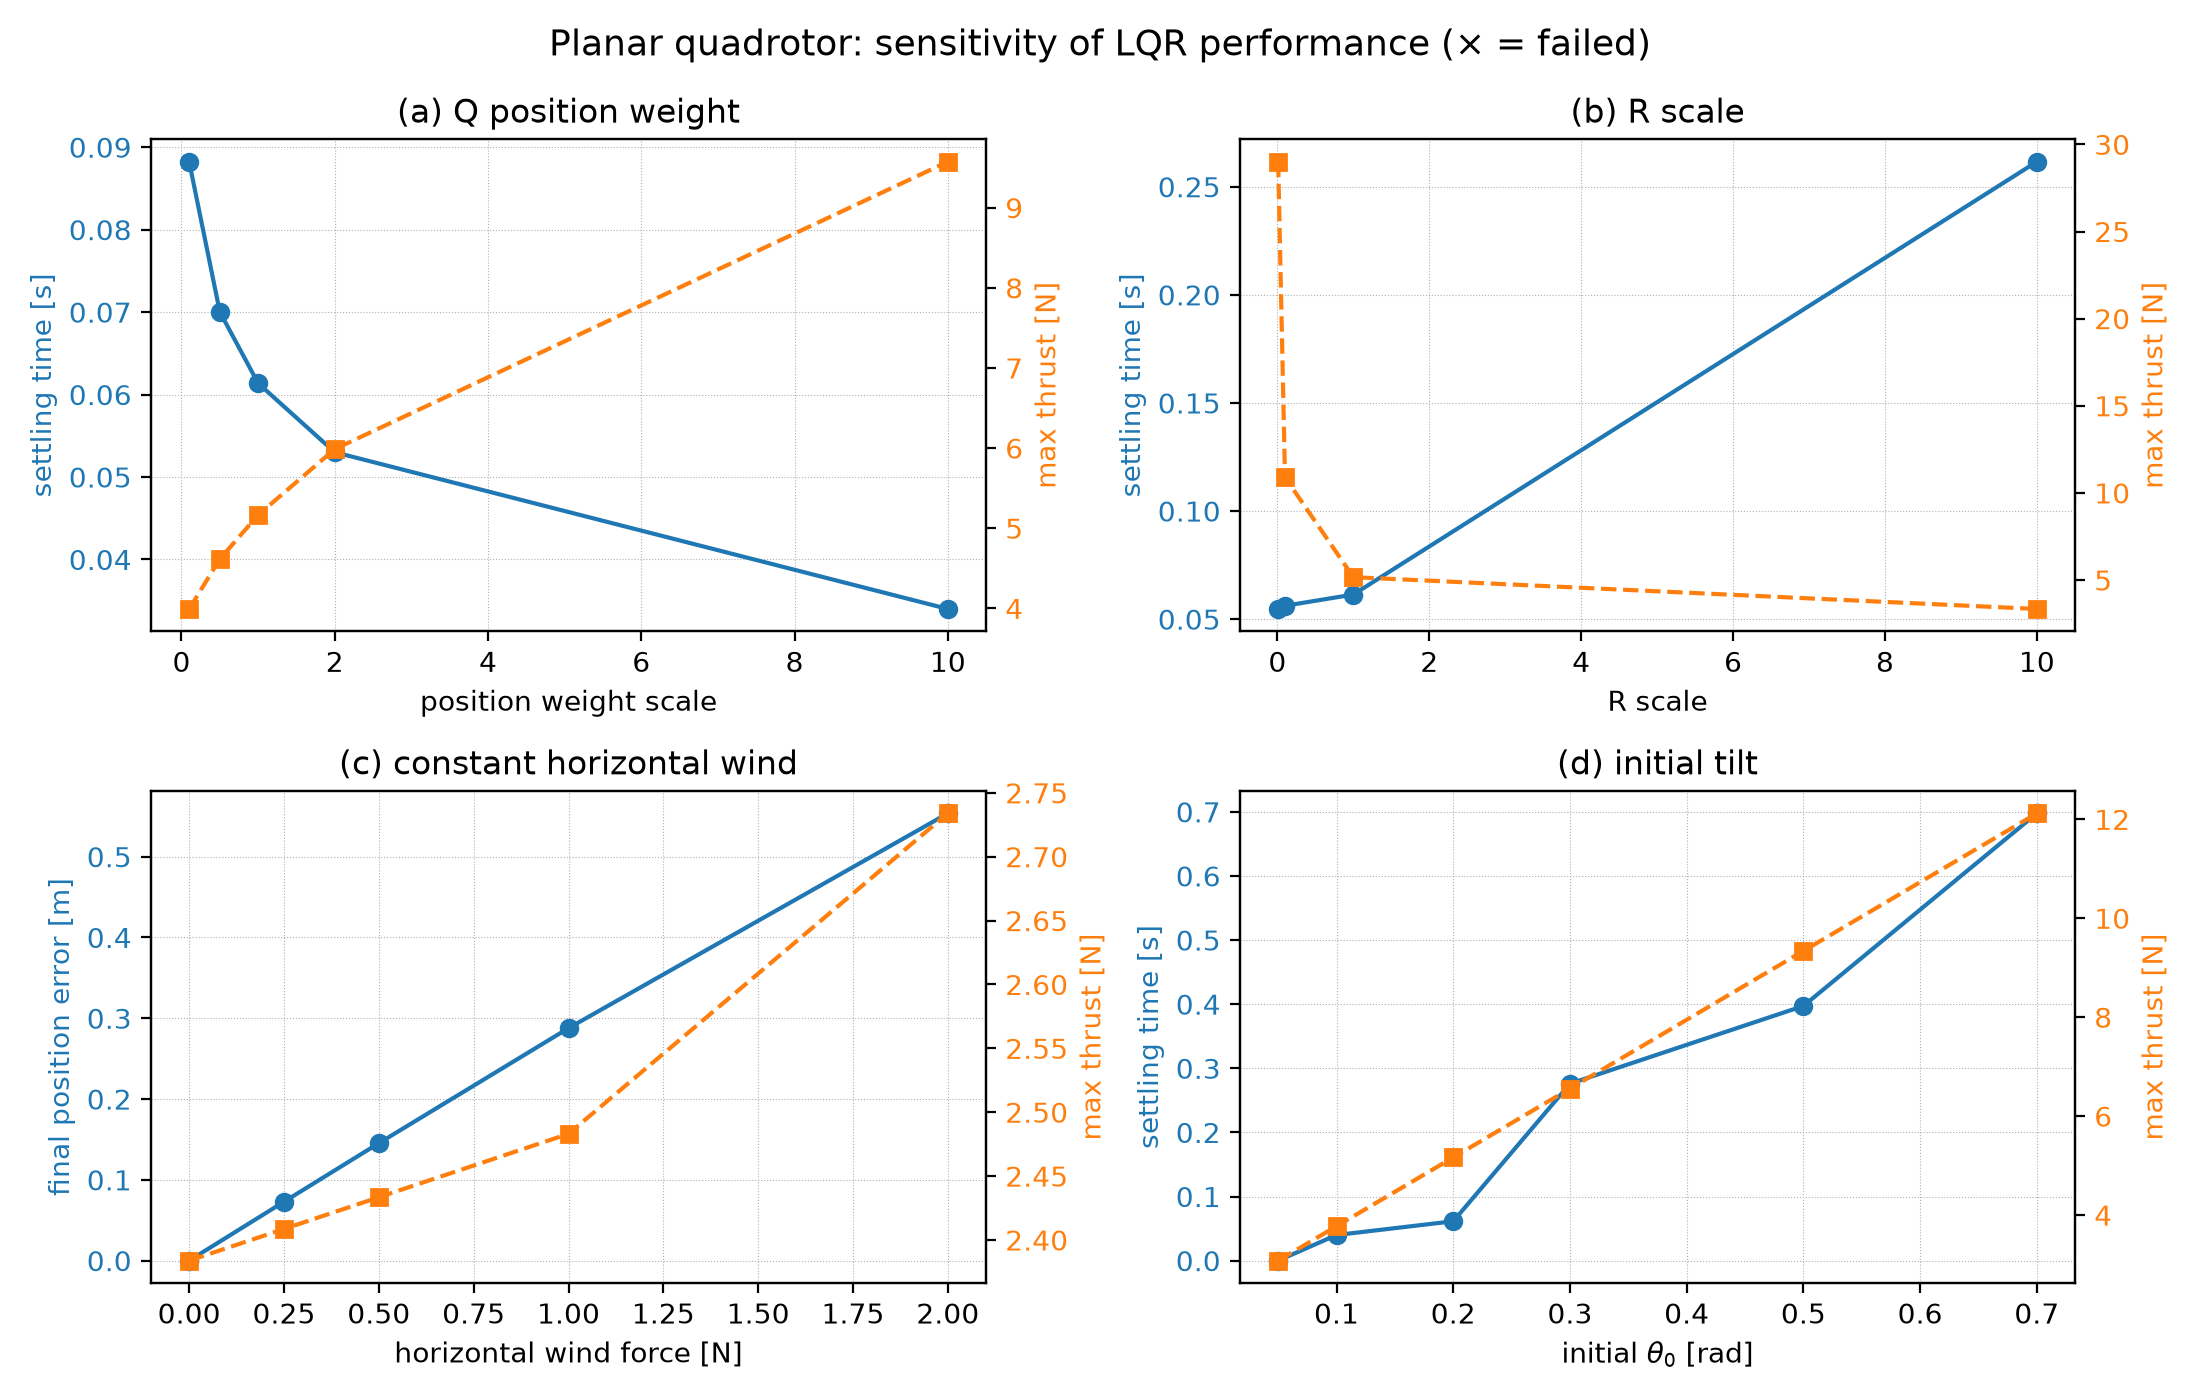
\includegraphics[width=0.95\textwidth]{quad_fig2_planar_sensitivity.png}
  \caption{Planar quadrotor sensitivity: (a) $\Q$ position weight,
  (b) $\R$ scale, (c) constant horizontal wind, (d) initial tilt.  The
  crosses denote failed runs; in (c) the nonzero steady-state offset is the
  expected consequence of no integral action.}
  \label{fig:planar_sens}
\end{figure}

\subsection{3D quadrotor}

For the 3D model the state is
\begin{equation}
\x=[x,y,z,\phi,\theta,\psi,\dot x,\dot y,\dot z,p,q,r]^\top
\end{equation}
with four propeller forces $u_1,\dots,u_4$.  The Drake model has mass
$m=0.775$ kg and inertia
$\operatorname{diag}(0.0015,0.0025,0.0035)$ kg\,m$^2$.  Hover at $(0,0,1)$
requires $u_i=mg/4$.  The closed-loop poles of the LQR below are
$-141.4,\,-84.8,\,-13.6,\,-3.25,\,-3.16,\,-3.16,\,-2.40\pm1.55j$ and
$-2.21\pm2.22j$ (each complex pair twice).  Following the textbook notebook,
we use
\begin{equation}
\Q=\operatorname{diag}(10,\dots,10,1,\dots,1),
\qquad \R=I_4 .
\end{equation}
The official \texttt{StabilizingLQRController} and our own LQR give the same
baseline performance from
$(0,0,1,0.2,0.1,0,0,\dots,0)$: final position error $<10^{-5}$ m, peak attitude
deviation 0.2 rad, settling time 1.08 s and peak thrust 3.0 N.

\begin{figure}[htbp]
  \centering
  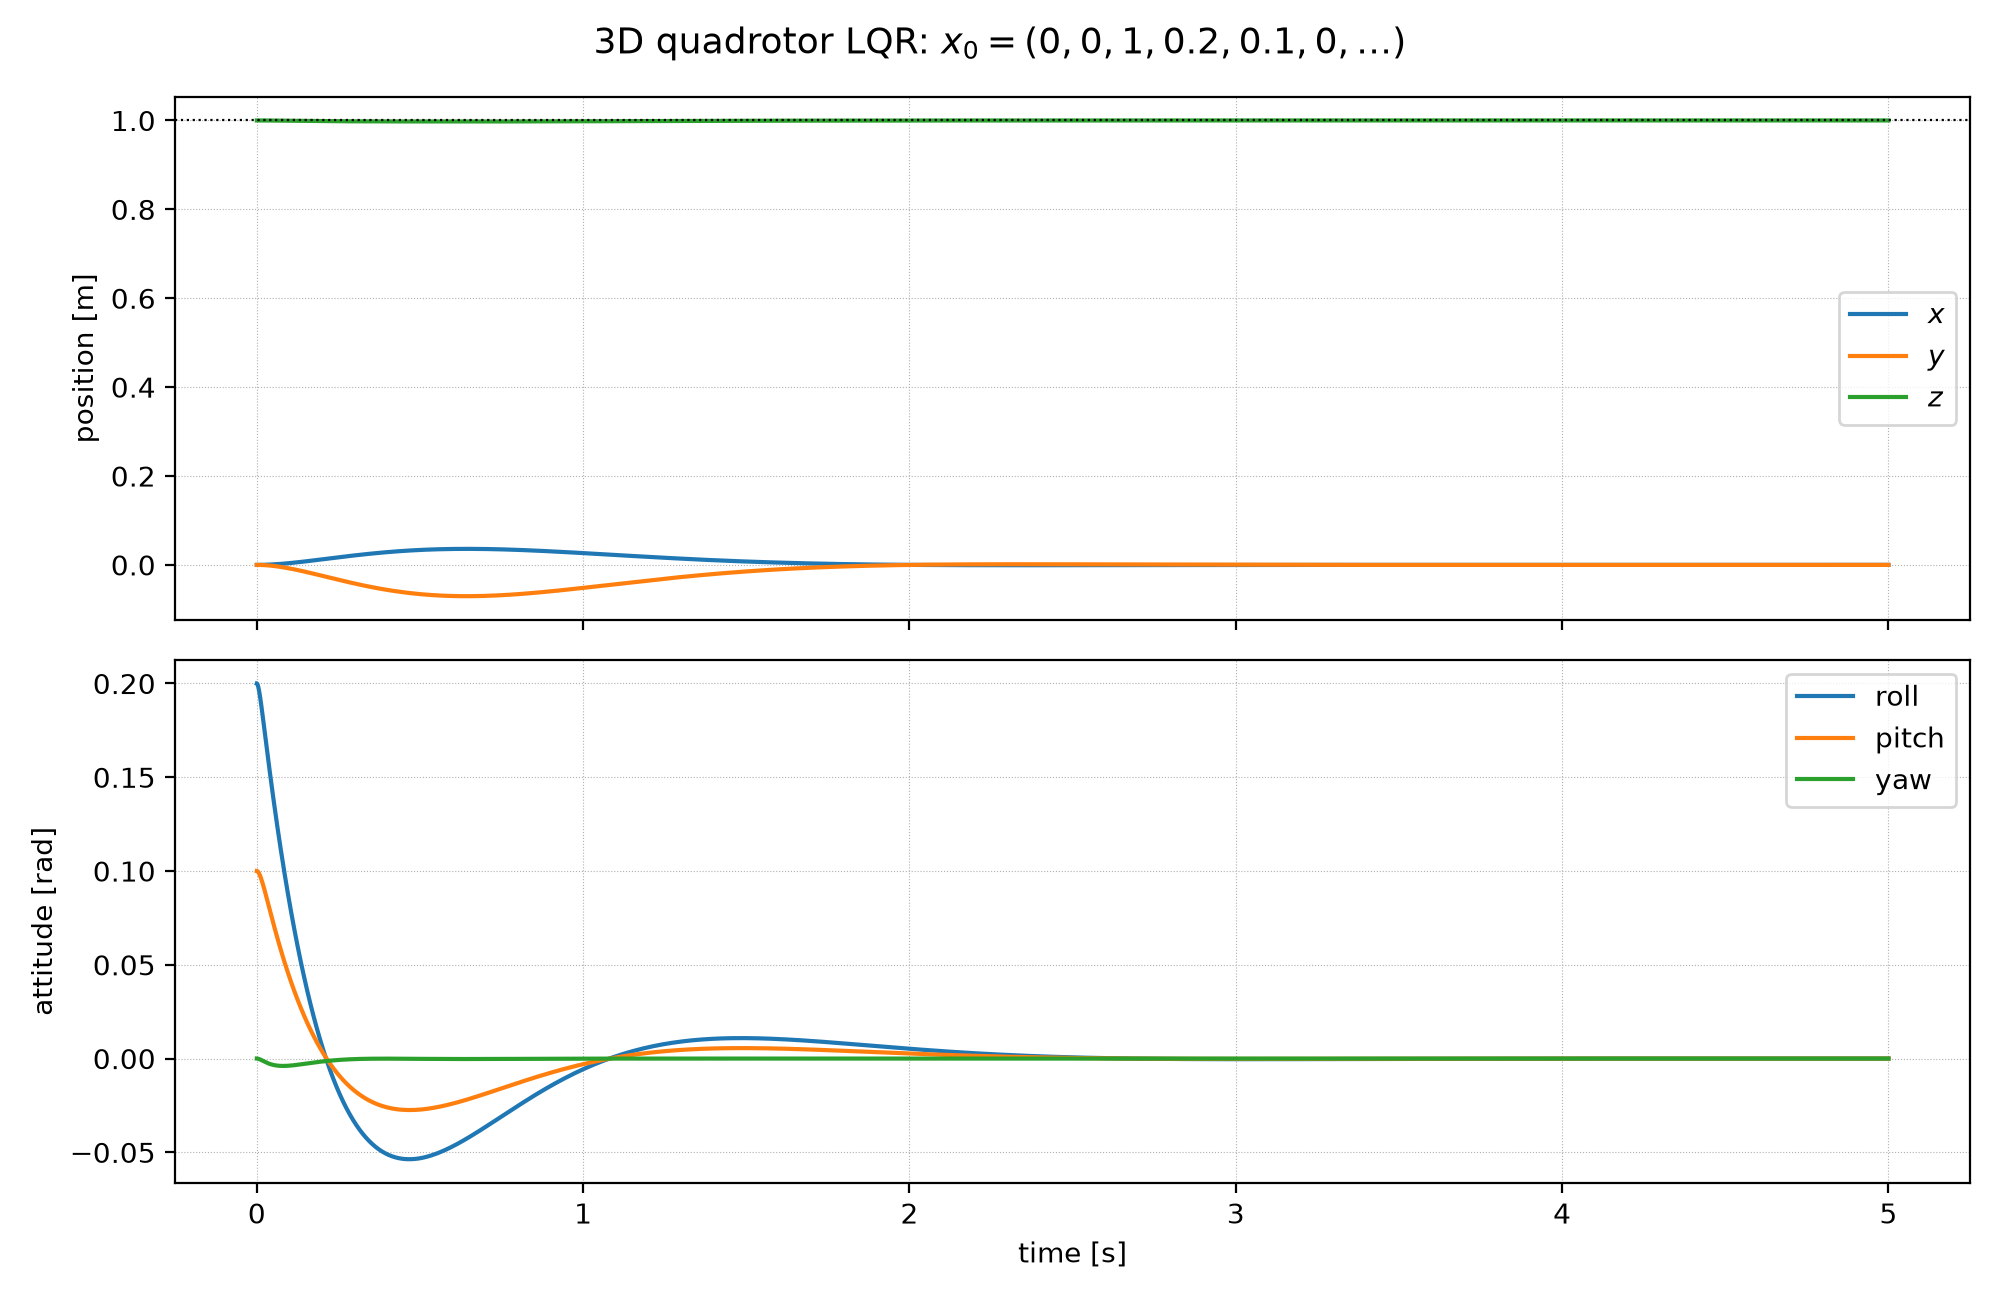
\includegraphics[width=0.9\textwidth]{quad_fig3_quad3d_baseline.png}
  \caption{3D quadrotor LQR from a $0.2$ rad roll and $0.1$ rad pitch
  perturbation.  Position (top) and attitude (bottom).}
\end{figure}

\paragraph{Sensitivity.}  Figure~\ref{fig:quad3d_sens} reports the settling
time and peak thrust for variations of $\Q$, $\R$ and the initial tilt:
\begin{itemize}[leftmargin=1.4em]
  \item increasing the position/attitude weight reduces the settling time
        from 2.02 s to 0.08 s but raises the peak thrust from 2.68 N to
        3.99 N;
  \item increasing $\R$ reduces the peak thrust from 12.7 N to 2.26 N with
        only a small increase in settling time;
  \item larger initial tilts require more thrust and take longer to settle
        (1.44 s at 0.5 rad), but all tested cases recover.
\end{itemize}

\begin{figure}[htbp]
  \centering
  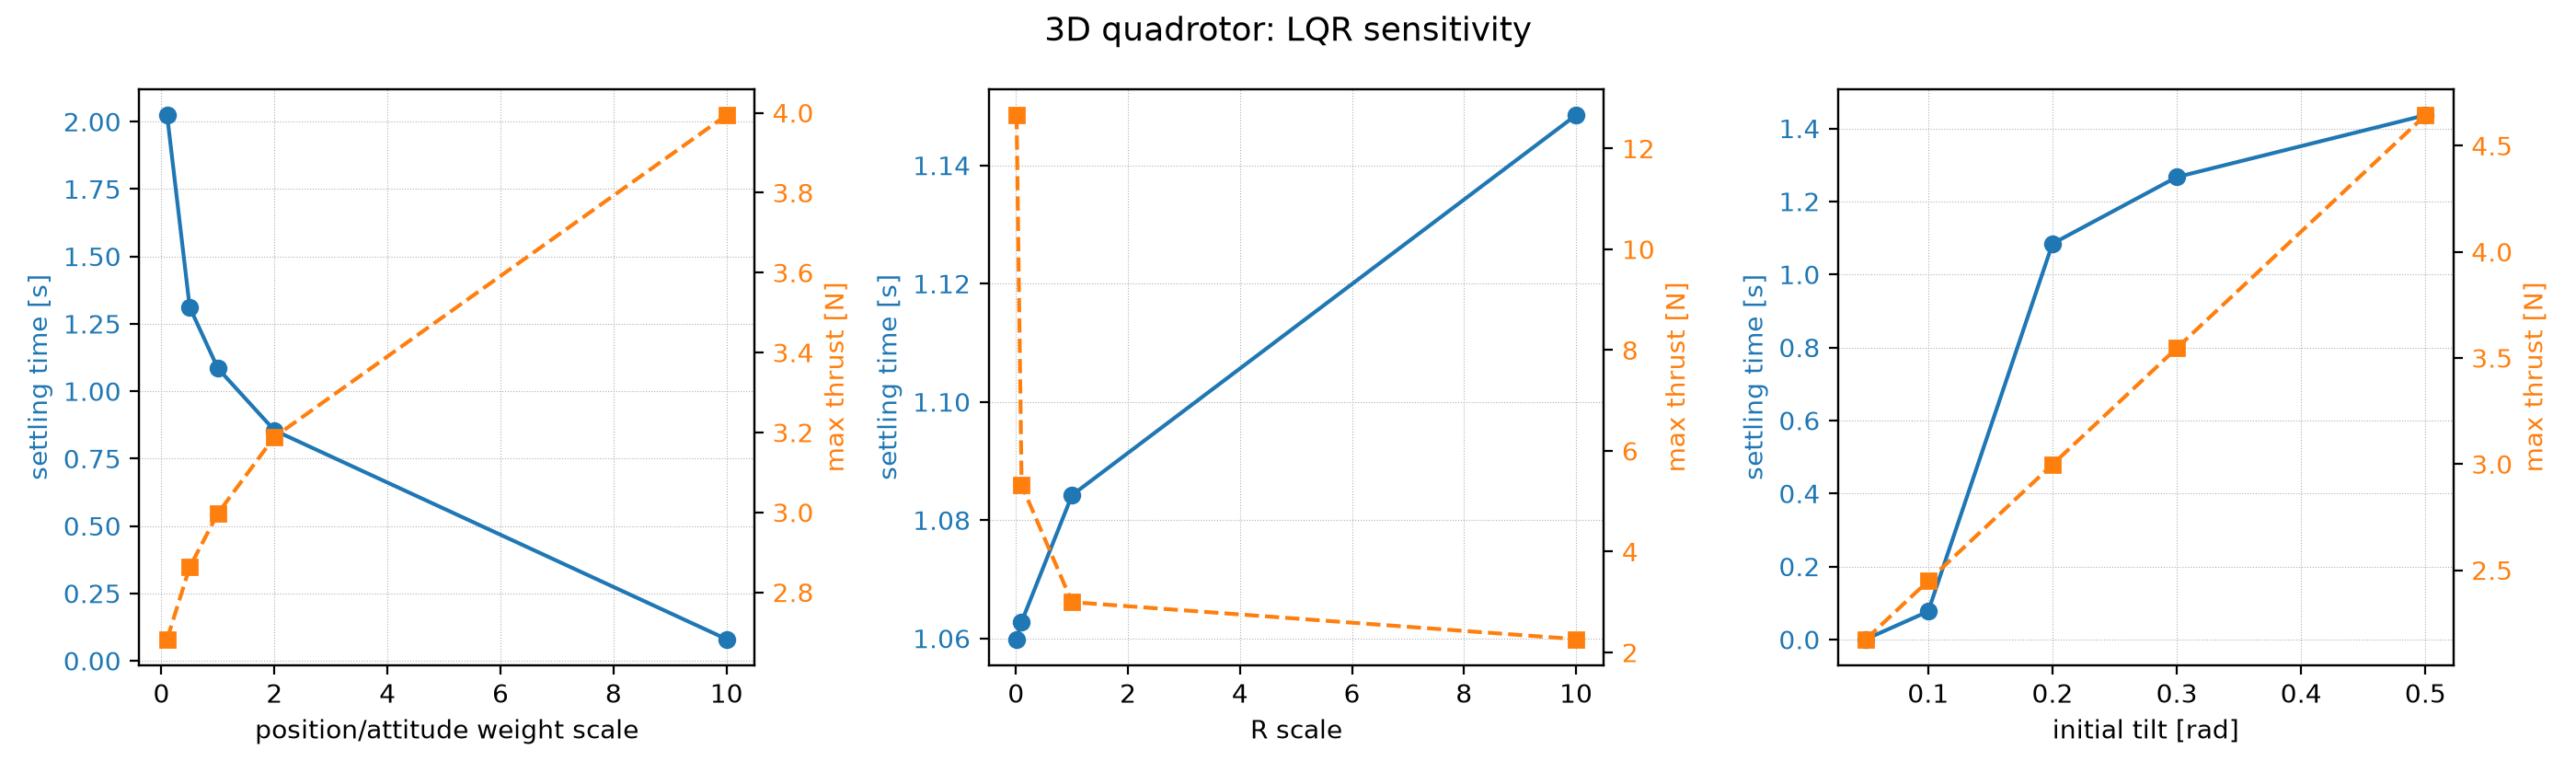
\includegraphics[width=0.95\textwidth]{quad_fig4_quad3d_sensitivity.png}
  \caption{3D quadrotor sensitivity: settling time (left axis) and peak thrust
  (right axis) vs.\ $\Q$ weight, $\R$ scale and initial tilt.}
  \label{fig:quad3d_sens}
\end{figure}

\textbf{Comment.}  LQR works out of the box for the quadrotor because the
linearisation is taken around a \emph{non-zero} thrust that balances gravity.
The vehicle is underactuated (four inputs for six degrees of freedom), but the
hover equilibrium is stabilisable.  The $\Q/\R$ trade-off is the usual one:
aggressive attitude/position weighting gives fast response at the price of
thrust; large $\R$ is gentle but slow.  Since LQR has no integral action, a
constant wind produces a steady-state position error; rejecting it would
require integral action, a disturbance observer or MPC.

%=====================================================================
\section{Section 3.8: Exercise 3.1}
%=====================================================================

\subsection{Nonlinear dynamics and linearisation}

For the cart-pole with $m_c=m_p=1$, $l=1$, $g=9.81$ and
$\x=[x,\theta,\dot x,\dot\theta]^\top$, the equations used in the notebook are
\begin{align}
\ddot x &= \frac{u+\sin\theta\left(\dot\theta^2+g\cos\theta\right)}
                {1+\sin^2\theta},\\
\ddot\theta &= \frac{-u\cos\theta-\dot\theta^2\cos\theta\sin\theta
                -2g\sin\theta}{1+\sin^2\theta}.
\end{align}
At the upright equilibrium $\x^\star=[0,\pi,0,0]^\top$,
\begin{equation}
\A_{\mathrm{lin}}=\begin{bmatrix}
0&0&1&0\\0&0&0&1\\0&9.81&0&0\\0&19.62&0&0
\end{bmatrix},
\qquad
\B_{\mathrm{lin}}=\begin{bmatrix}0\\0\\1\\1\end{bmatrix}.
\end{equation}

\begin{figure}[htbp]
\centering
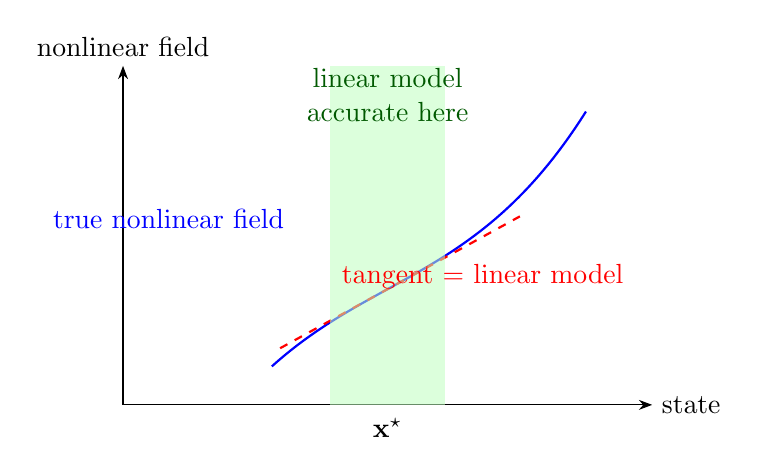
\begin{tikzpicture}[>=Stealth,scale=1.05]
  \draw[->] (0,0)--(6.4,0) node[right] {state};
  \draw[->] (0,0)--(0,4.1) node[above] {nonlinear field};
  \draw[thick,blue] plot[domain=1.8:5.6,samples=100]
       (\x,{0.06*(\x-3.2)^3+0.55*(\x-3.2)+1.4});
  \draw[dashed,red,thick] plot[domain=1.9:4.8]
       (\x,{0.55*(\x-3.2)+1.4});
  \fill[green!25,opacity=0.55] (2.5,0) rectangle (3.9,4.1);
  \node at (3.2,-0.28) {$\x^\star$};
  \node[green!35!black,align=center] at (3.2,3.75)
       {linear model\\accurate here};
  \node[red] at (4.35,1.55) {tangent = linear model};
  \node[blue] at (0.55,2.25) {true nonlinear field};
\end{tikzpicture}
\caption{Why linearisation is local.  The red dashed line is the tangent
(linear model) at $\x^\star$; the blue curve is the true nonlinear field.
They agree near $\x^\star$ (green band) and diverge farther away.  The six
test points in the table below sample different distances from the
equilibrium.}
\label{fig:linearization_local}
\end{figure}

\begin{pitfall}[breakable=false,title={Do not use a linear controller everywhere}]
A linear controller is designed for the tangent at one point.  If the state
is far from that point, the real dynamics can differ so much that the
controller no longer helps.  In this exercise the controller works from
$\theta=0.99\pi$, $0.90\pi$ and $0.85\pi$, but fails from $\theta=\pi/2$ and
from the downward equilibrium $\theta=0$.  The failure is not numerical: the
linear model is simply the wrong model there.  This is also why a real
cart-pole needs a swing-up controller before the LQR can take over.
\end{pitfall}

\subsection{Linearisation error}

\begin{table}[htbp]
\centering
\caption{Linearisation error for the six conditions of the notebook.}
\begin{tabular}{ccccc}
\toprule
Case & $\x$ & $u$ & $e(\x,u)$ & $\|f(\x,u)\|$ \\
\midrule
0 & $[0,0.99\pi,0,0]$ & 0 & 0.0009 & 0.688 \\
1 & $[0,0.90\pi,0,0]$ & $-10$ & 2.354 & 18.450 \\
2 & $[0,0.85\pi,0,0]$ & 0 & 2.289 & 8.085 \\
3 & $[0,0.50\pi,0,0]$ & 0 & 26.054 & 9.810 \\
4 & $[0,0,0,0]$ & 0 & 68.913 & 0 \\
5 & $[1,\pi,0,0]$ & 10 & $\approx0$ & 14.142 \\
\bottomrule
\end{tabular}
\end{table}

\begin{figure}[htbp]
  \centering
  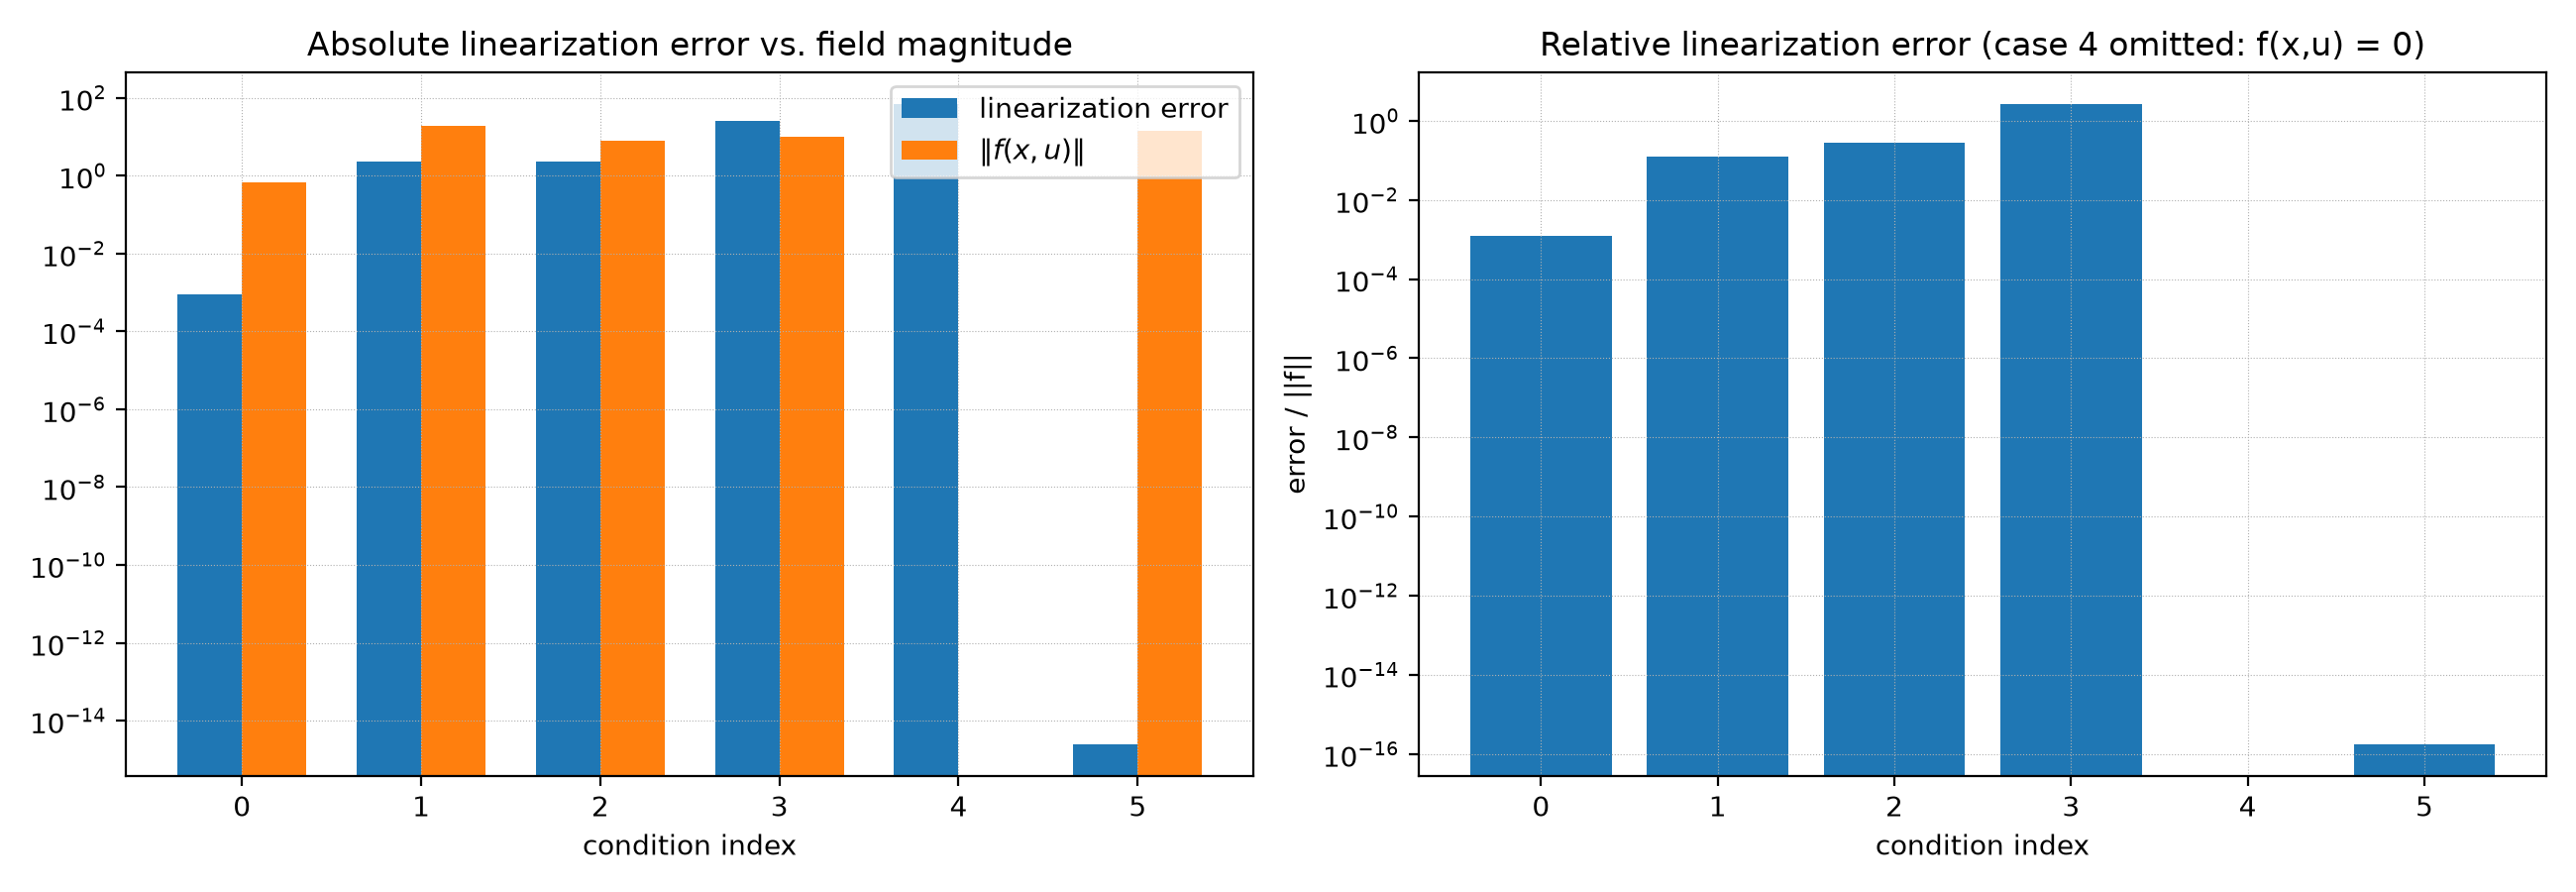
\includegraphics[width=0.9\textwidth]{s38_lin_error.png}
  \caption{Absolute and relative linearisation errors.  The linear model is
  accurate only near the upright equilibrium.}
\end{figure}

\textbf{Comments.}  The linear model is not valid at all points: at
$\theta=\pi/2$ the error is 2.66 times the field magnitude, and at
$\theta=0$ the error is 68.9.  When $\theta\neq\pi$, the error depends on
$u$ because the nonlinear input gains are
$u/(1+\sin^2\theta)$ and $-u\cos\theta/(1+\sin^2\theta)$, whereas the linear
model uses the constants $(1,1)$.  The cart position $x$ does not appear in
$f$, so it does not affect the error.  This is why case~1 has a larger error
than case~2 even though its angle is closer to $\pi$: it has a large input.

\subsection{LQR and recovery}

With $\Q=I_4$, $\R=1$ the gain is
\begin{equation}
K=[\,-1.0000,\;51.0612,\;-2.7221,\;12.8277\,],
\qquad u=-K(\x-\x^\star),
\end{equation}
and the closed-loop poles are
\begin{equation}
-5.0417,\quad -3.9438,\quad -0.5600\pm0.4239j.
\end{equation}
A 5 s nonlinear simulation from the six initial states recovers from
\begin{equation}
\boxed{\texttt{system\_recovers\_from\_states}=[0,1,2,5]}.
\end{equation}
Cases 0--2 are close to the upright point; case 5 has $\theta=\pi$ and only a
cart offset, which is linearly controllable.  Case 3 ($\theta=\pi/2$) and
case 4 ($\theta=0$) are outside the linearisation region and the controller
fails, as predicted by the error table.

\begin{figure}[htbp]
  \centering
  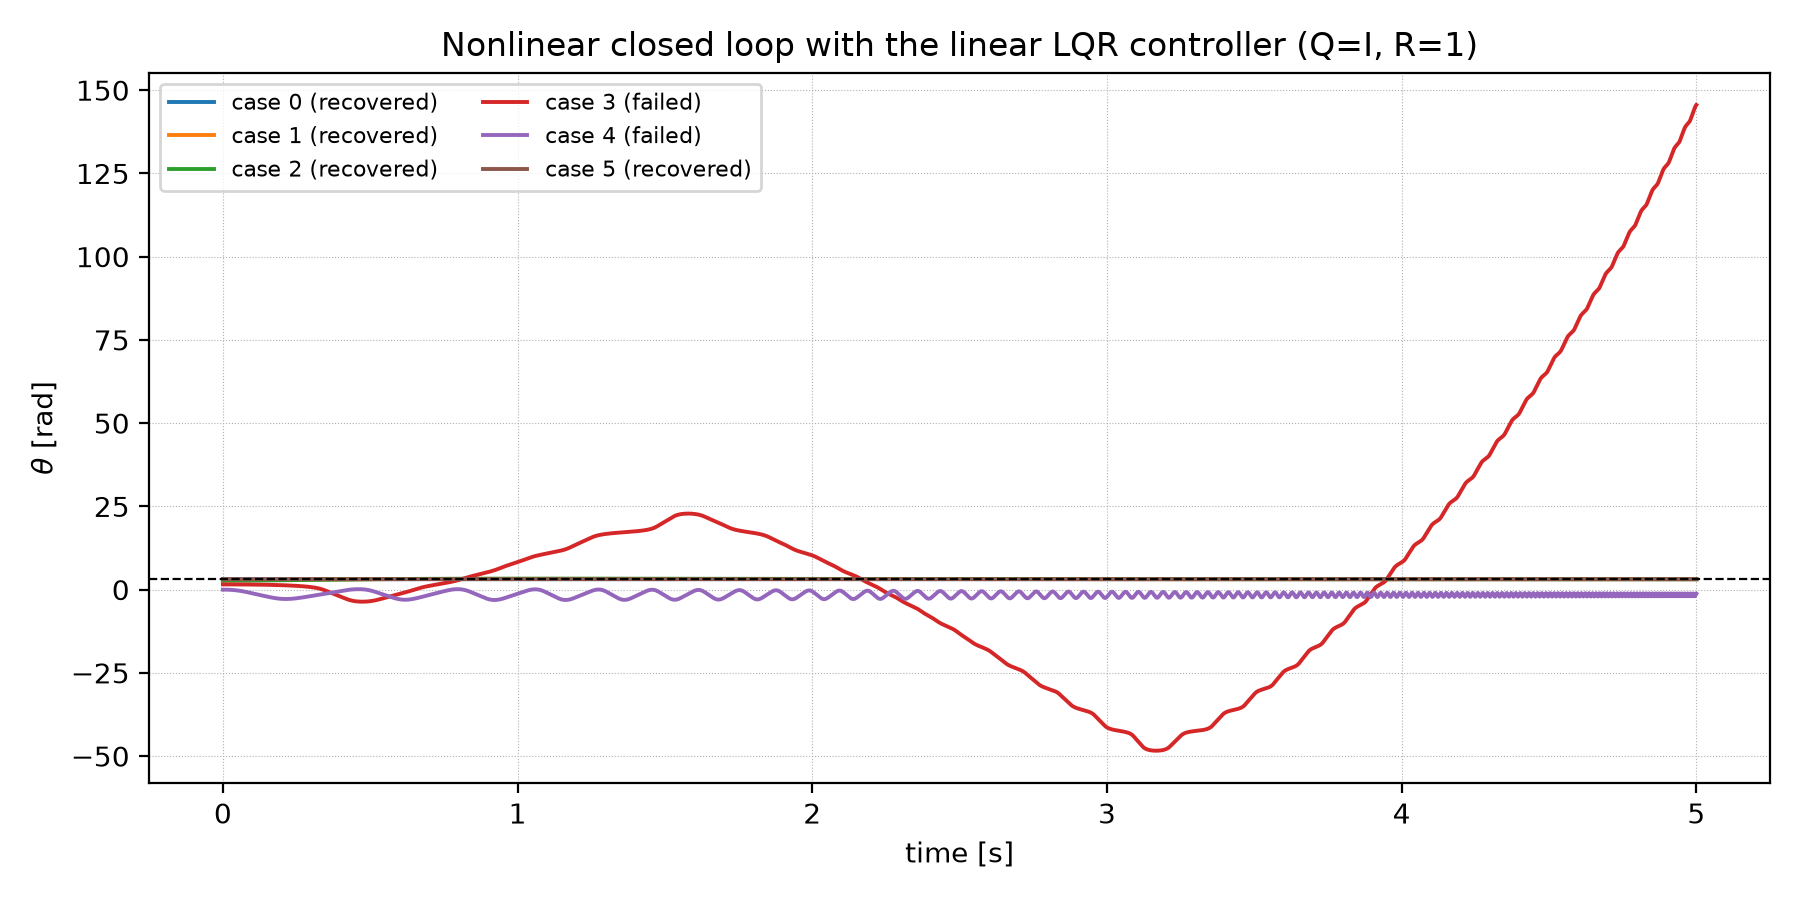
\includegraphics[width=0.82\textwidth]{s38_closed_loop_theta.png}
  \caption{Closed-loop angle histories for the six initial states.  Only
  cases 0, 1, 2 and 5 converge to the upright position.}
\end{figure}

%=====================================================================
\section{Section 3.8: Exercise 3.2}
%=====================================================================

\subsection{URDF construction}

The single cart-pole is built from three XML blocks:
\begin{itemize}[leftmargin=1.4em]
  \item \textbf{links}: a base with mass 1 at its origin, a pendulum link whose
        ball (mass 1) is at $z=-1$, a spherical visual of radius 0.05 and a
        cylindrical rod of length 1 and radius 0.01 centred at $z=-0.5$;
  \item \textbf{joints}: a prismatic joint $x$ from the world to the base, and
        a continuous joint $\theta_0$ from the base to the pendulum, with
        origin $(0,0,0)$ and axis $(0,-1,0)$;
  \item \textbf{transmission}: a simple transmission that maps the actuator
        force to the prismatic joint.
\end{itemize}

The unstable equilibrium is $\x^\star=[0,\pi,0,0]^\top$.

\subsection{Double pendulum}

The second joint is attached at the ball of the first pendulum:
\texttt{origin xyz="0 0 -1"} in the \texttt{pendulum0} frame.  The second
link has its ball at $z=+1$ in its own frame.  Hence, for $\theta_1=0$ the
second pendulum points back towards the cart and exactly overlaps the first;
for $\theta_0=\theta_1=\pi$ both pendula stand upright one above the other.
The unstable equilibrium is
\begin{equation}
\x^\star=[0,\pi,\pi,0,0,0]^\top.
\end{equation}

\begin{figure}[htbp]
\centering
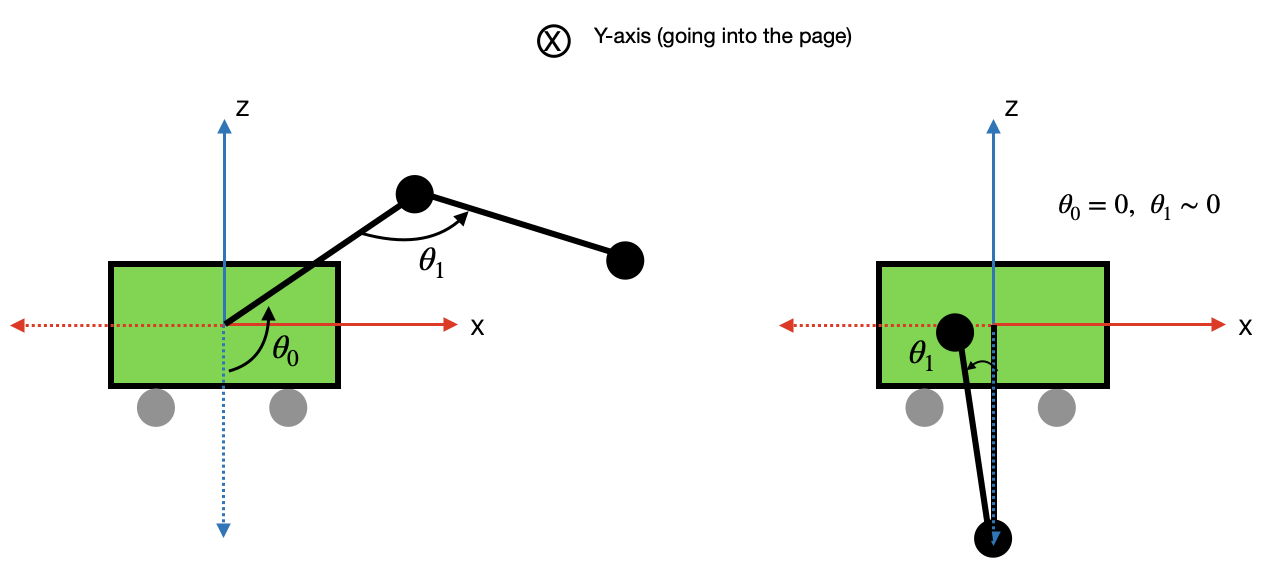
\includegraphics[width=0.9\textwidth]{double_pendulum_geometry.png}
\caption{Geometry of the double pendulum (textbook figure).  Left: general
configuration, with $\theta_0$ measured from the downward vertical and
$\theta_1$ measured relative to the first pendulum.  Right: the home
configuration $\theta_0=\theta_1=0$.  The second pendulum points back towards
the cart and overlaps the first; this is exactly what the notebook asks you
to observe.}
\label{fig:double_geom}
\end{figure}

\begin{recipe}[title={Reading URDF frames (the part that is easy to get wrong)}]
A URDF is a chain of \emph{frames}, not a chain of absolute coordinates.
\begin{enumerate}[leftmargin=1.4em,itemsep=2pt]
  \item The \texttt{<origin>} of a joint is written in the \emph{parent link}
        frame.  Here \texttt{theta1} has origin $(0,0,-1)$ in
        \texttt{pendulum0}, so the joint sits at the ball of pendulum~0.
  \item The child link frame is the joint frame.  Therefore the inertial and
        visual origins of \texttt{pendulum1} are written in the
        \texttt{pendulum1} frame, i.e.\ relative to that joint.
  \item In the home configuration $\theta_1=0$, the child frame is not
        rotated.  Putting the ball at $z=+1$ in this frame makes it go from
        the joint at $z=-1$ back up to $z=0$: the two rods overlap.
  \item At $\theta_0=\theta_1=\pi$, pendulum~0 points up (ball at $z=+1$);
        the second joint is at that ball, and $\theta_1=\pi$ turns the second
        rod so its ball is at $z=+2$.  Both links stand upright, one above the
        other.
\end{enumerate}
\end{recipe}

\begin{lstlisting}[language=XML,caption={Key part of the double-pendulum URDF.}]
<link name="pendulum1">
  <inertial>
    <origin xyz="0 0 1" rpy="0 0 0" />
    <mass value="1" />
    <inertia ixx="0" ixy="0" ixz="0" iyy="0" iyz="0" izz="0" />
  </inertial>
  <visual>
    <origin xyz="0 0 1" />
    <geometry><sphere radius="0.05" /></geometry>
  </visual>
  <visual>
    <origin xyz="0 0 0.5" />
    <geometry><cylinder length="1" radius="0.01" /></geometry>
  </visual>
</link>
<joint name="theta1" type="continuous">
  <parent link="pendulum0" />
  <child link="pendulum1" />
  <origin xyz="0 0 -1" />
  <axis xyz="0 -1 0" />
</joint>
\end{lstlisting}

\subsection{LQR and results}

The LQR is synthesised directly from the nonlinear \texttt{MultibodyPlant} at
$\x^\star$:
\begin{lstlisting}[language=Python,caption={Wiring the LQR controller.}]
context = cartpole.CreateDefaultContext()
context.get_mutable_continuous_state_vector().SetFromVector(x_star)
cartpole.get_actuation_input_port().FixValue(context, [0])
input_i = cartpole.get_actuation_input_port().get_index()
lqr = LinearQuadraticRegulator(
    cartpole, context, Q, R, input_port_index=input_i)
lqr = builder.AddSystem(lqr)
builder.Connect(cartpole.get_state_output_port(), lqr.get_input_port(0))
builder.Connect(lqr.get_output_port(0), cartpole.get_actuation_input_port())
\end{lstlisting}

For the single pendulum with $\Q=\operatorname{diag}(10,10,1,1)$, $\R=1$:
\begin{equation}
K=[\,-3.1623,\;61.3987,\;-5.2854,\;16.1699\,],
\end{equation}
closed-loop poles $-4.8948,-4.0983,-0.9457\pm0.8075j$; after 5 s the angle
error is 0.0036 rad and the peak force is 19.3 N.  For the double pendulum
with $\Q=\operatorname{diag}(10,10,10,1,1,1)$ the gain is
\begin{equation}
K=[\,3.1623,\;-54.8416,\;-300.4370,\;7.4384,\;-54.0081,\;-68.9418\,],
\end{equation}
with closed-loop poles
$-7.5798,-6.1385,-3.6749,-3.4281,-0.7754\pm0.6611j$.  After 5 s the two angle
errors are 0.0142 rad and 0.0007 rad; the peak force is 66.6 N.  The cart is
still slowly returning to the origin, consistent with the slow pair of poles.

\begin{figure}[htbp]
  \centering
  \begin{subfigure}{0.49\textwidth}
    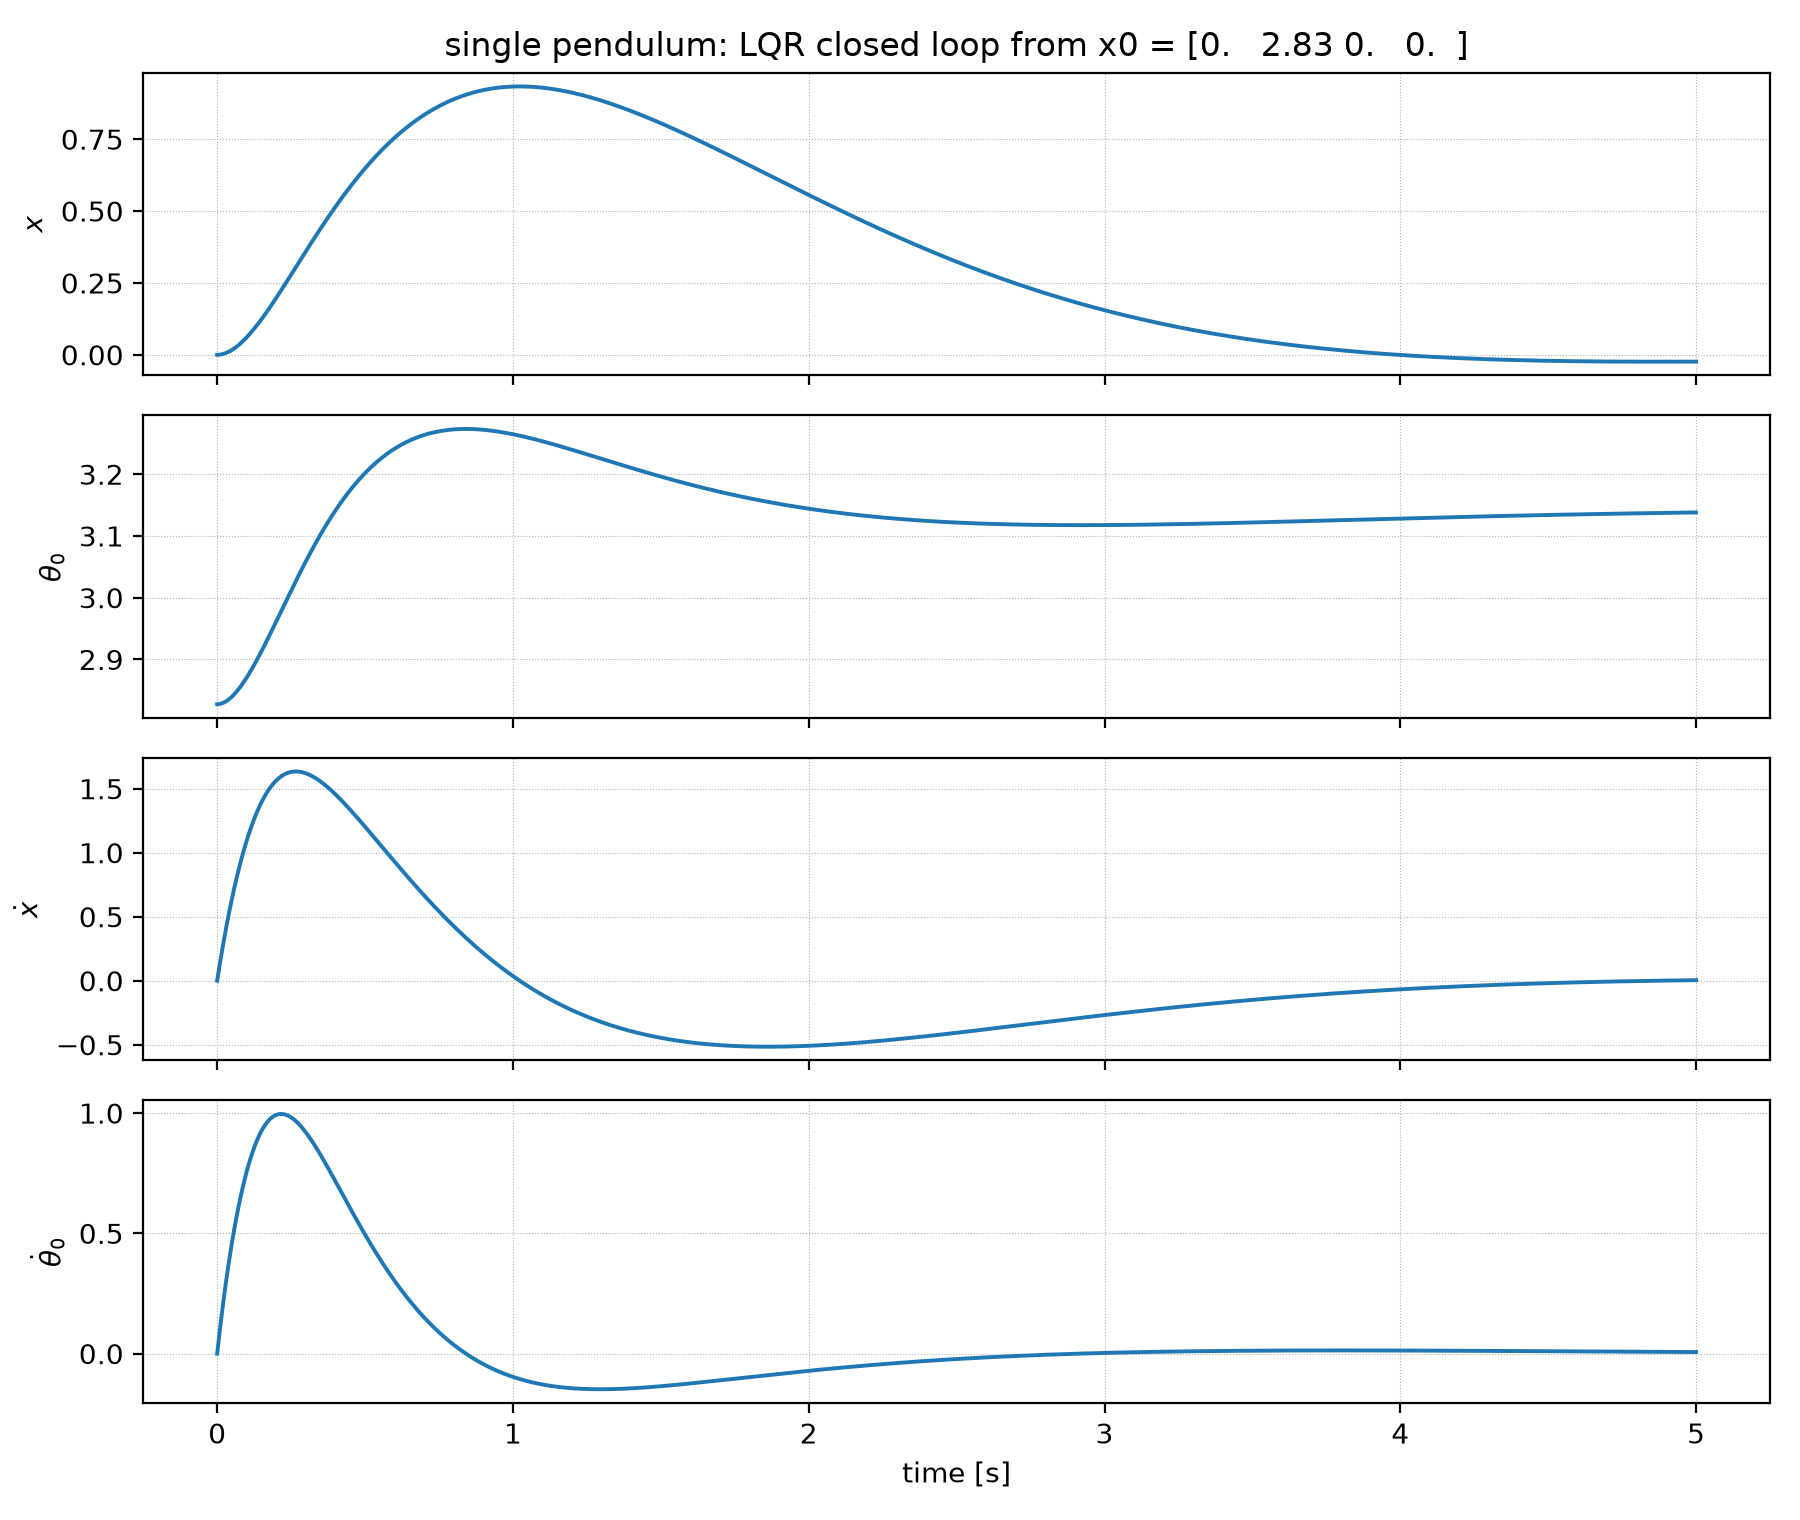
\includegraphics[width=\textwidth]{s38_single_balancing.png}
    \caption{Single pendulum.}
  \end{subfigure}\hfill
  \begin{subfigure}{0.49\textwidth}
    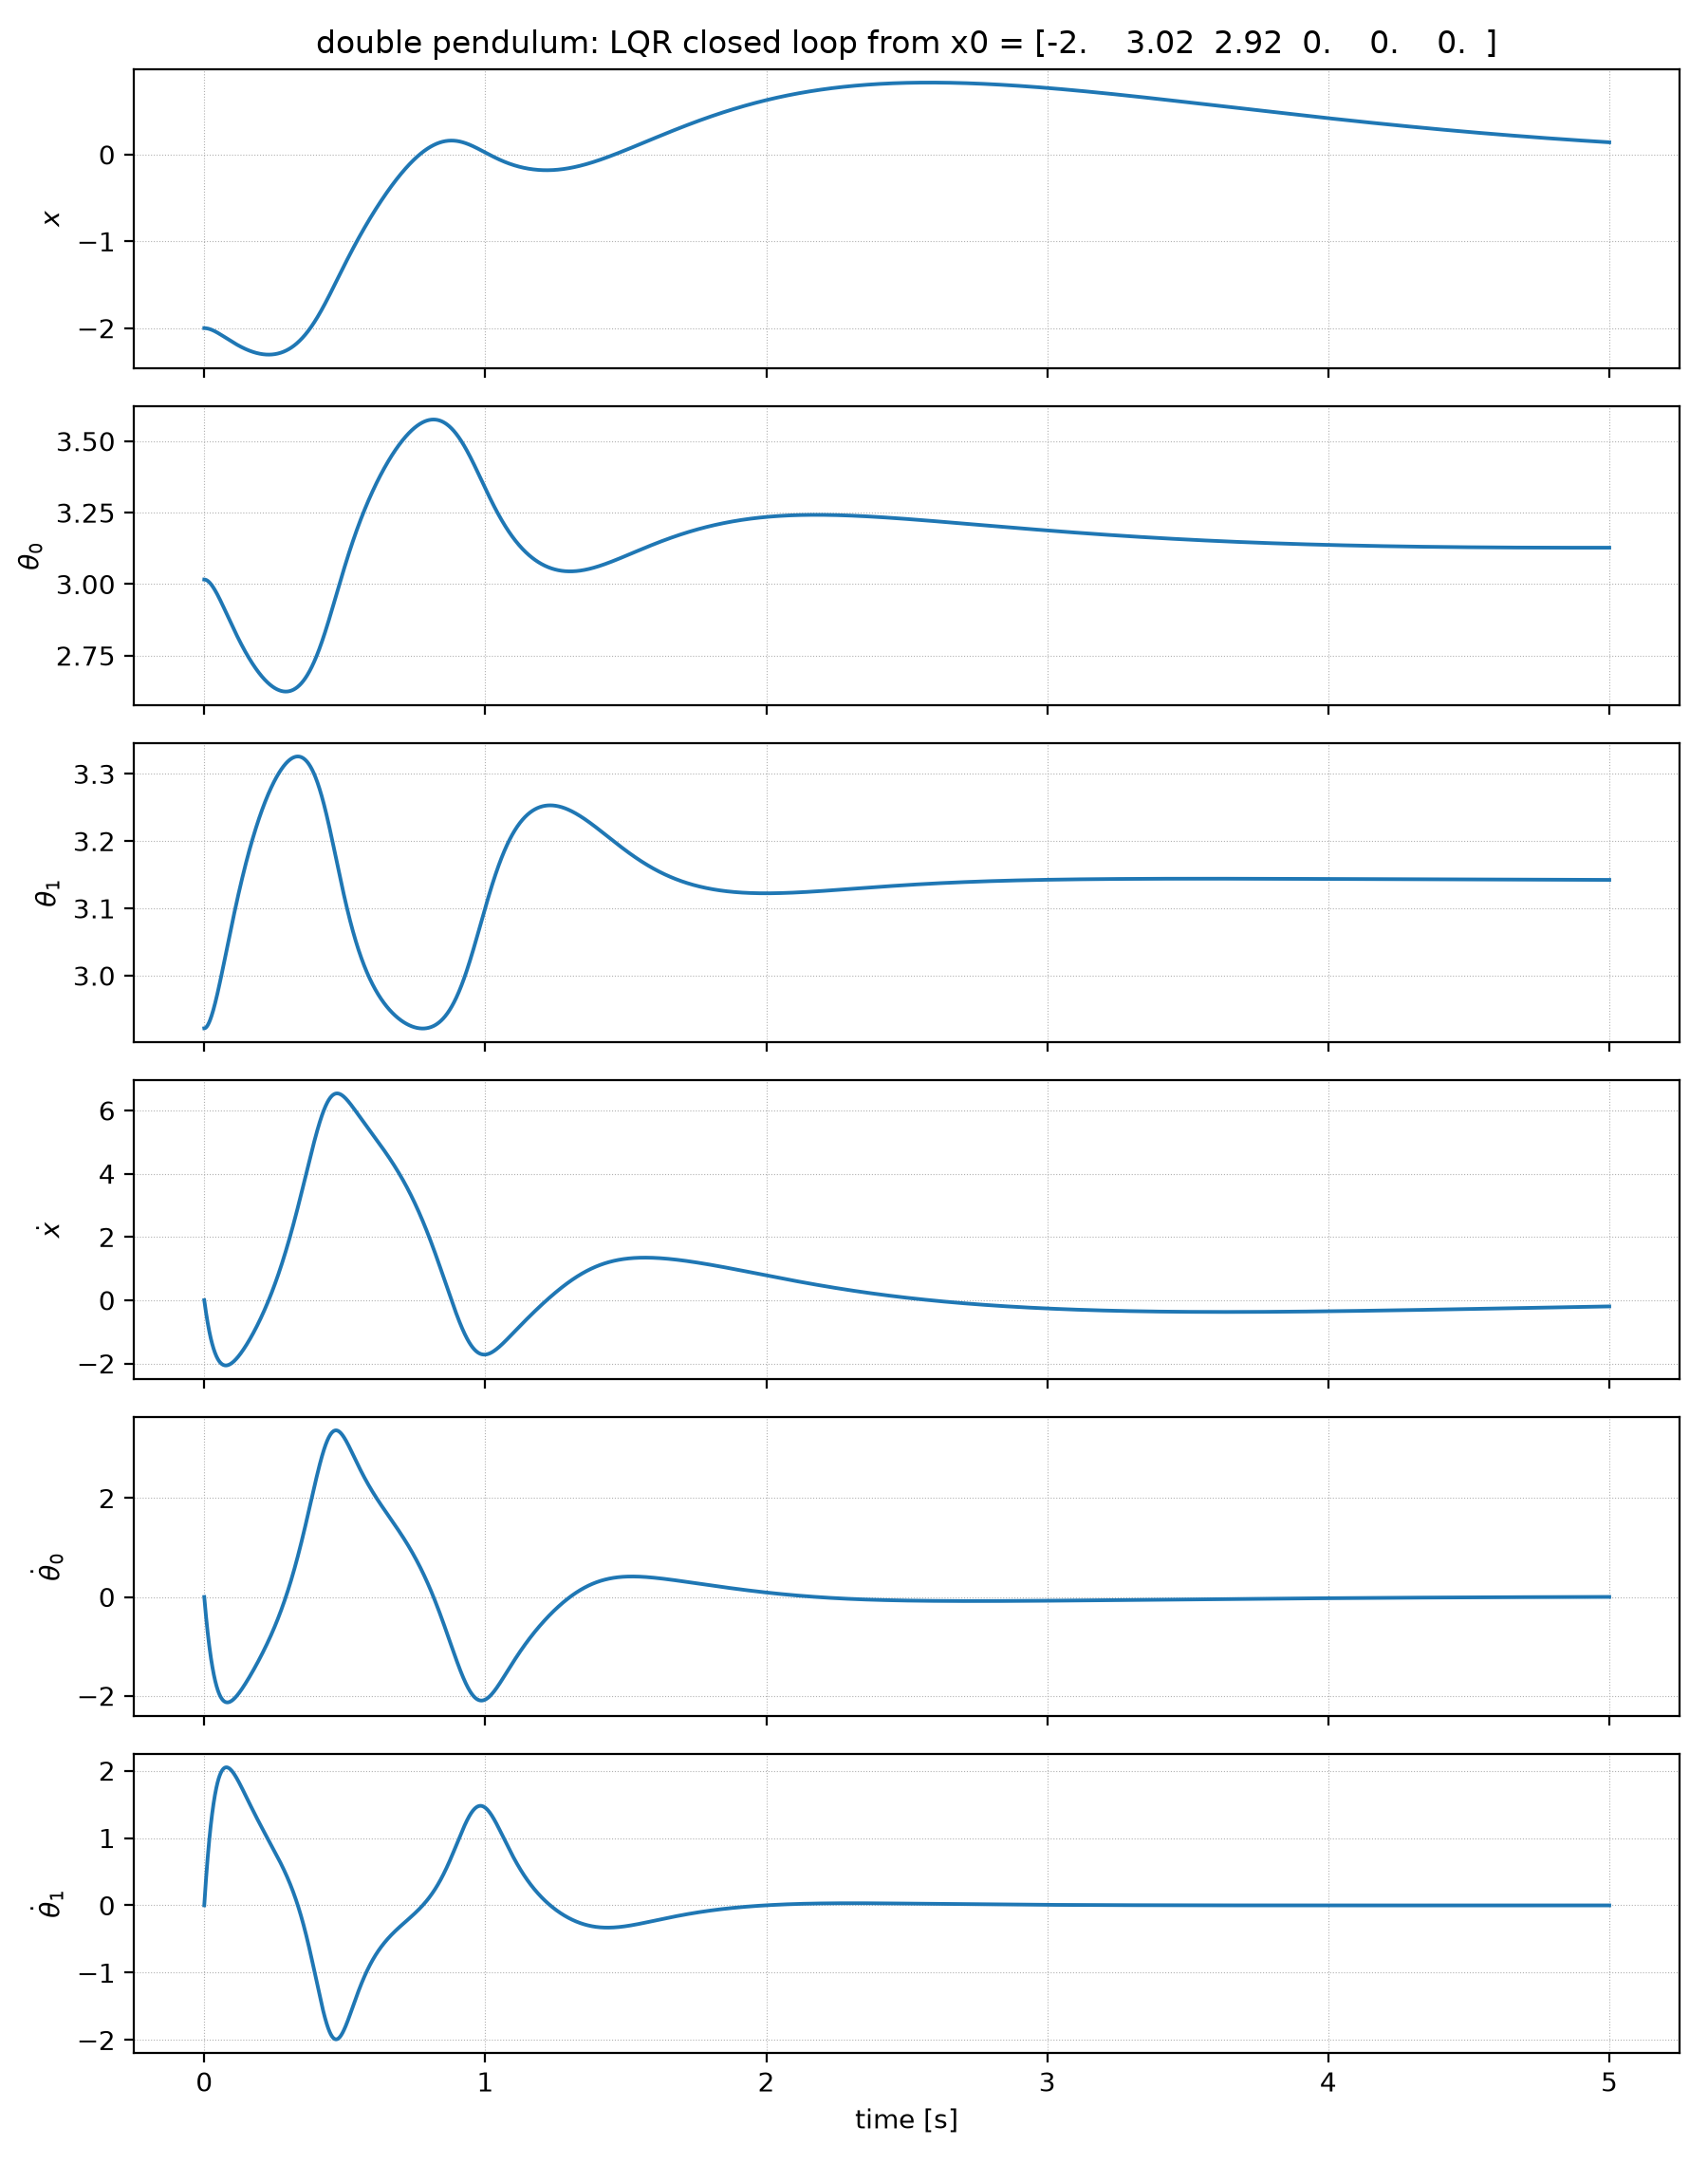
\includegraphics[width=\textwidth]{s38_double_balancing.png}
    \caption{Double pendulum.}
  \end{subfigure}
  \caption{LQR closed-loop simulations for the URDF models.}
\end{figure}

The autograder gives 12/12:
\begin{lstlisting}
Total score is 12/12.
Test x_star single pendulum        1/1
Test x_star double pendulum        1/1
Test single-pendulum dynamics      3/3
Test double-pendulum dynamics      3/3
Test single-pendulum LQR states    2/2
Test double-pendulum LQR states    2/2
\end{lstlisting}

%=====================================================================
\section{Section 3.8: Exercise 3.3}
%=====================================================================

\subsection{Discrete double integrator}

The dynamics are
\begin{equation}
x_1[n+1]=x_1[n]+x_2[n],\qquad
x_2[n+1]=x_2[n]+u[n],\qquad x_1,x_2,u\in\mathbb Z,
\end{equation}
so a transition from $s_{i,j}$ is
\begin{equation}
s_{i,j}\longmapsto (i+j,\;j+u).
\end{equation}

\begin{figure}[htbp]
  \centering
  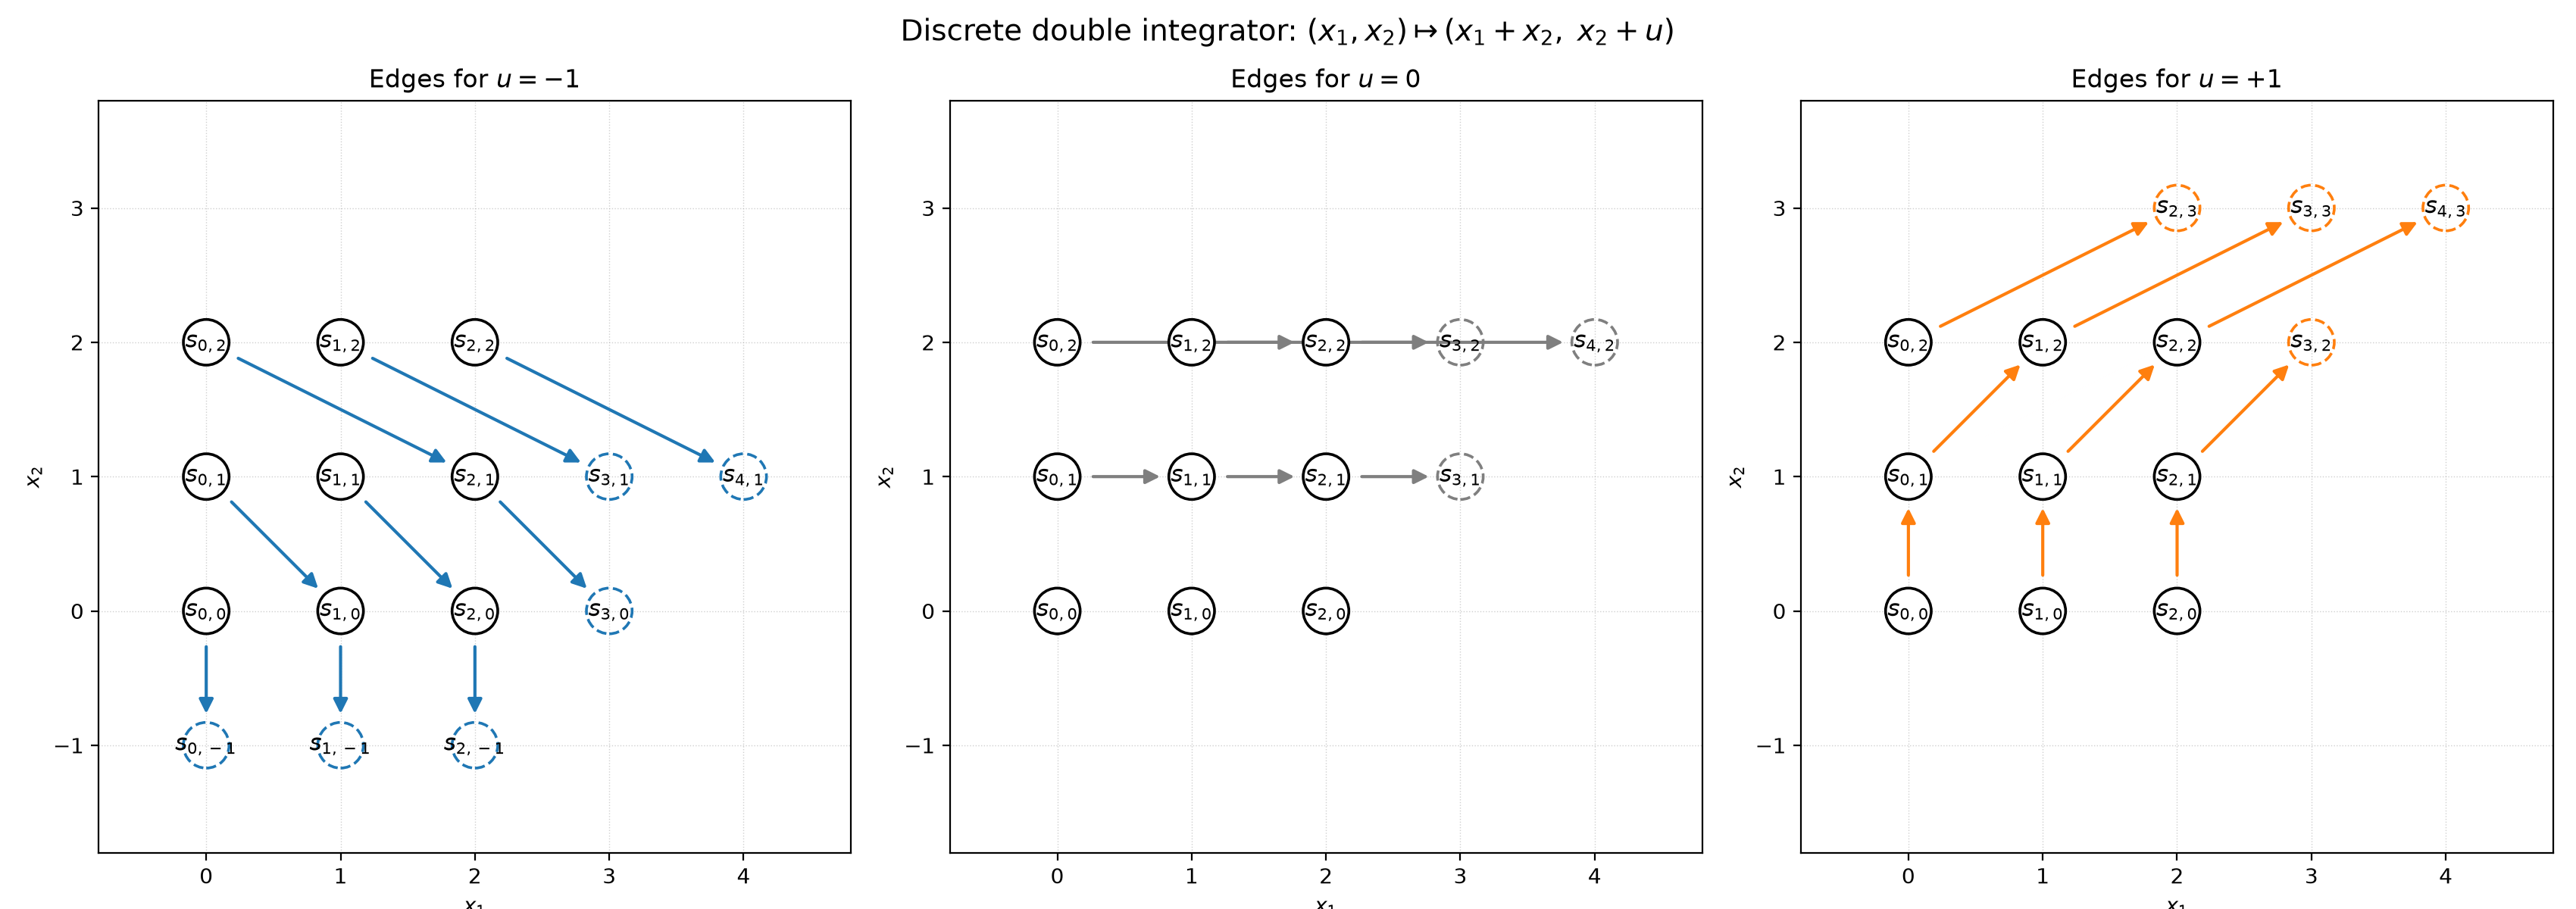
\includegraphics[width=0.98\textwidth]{s38_grid_graph.png}
  \caption{Edges of the graph for $u=-1,0,+1$.  The nine source nodes are
  drawn as solid circles; destinations outside the truncated grid are drawn
  as dashed circles.  For $u=0$ the three bottom nodes have self-loops.}
\end{figure}

\begin{figure}[htbp]
\centering
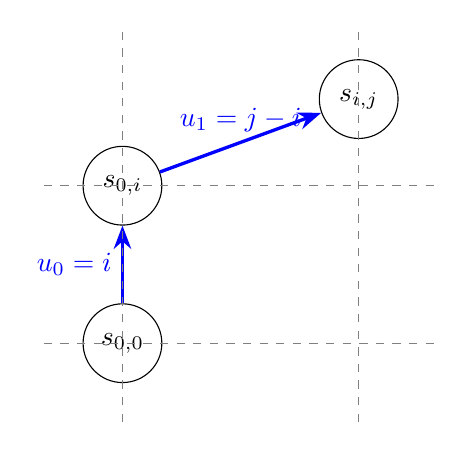
\begin{tikzpicture}[>=Stealth,scale=1.0,
  node/.style={circle,draw,minimum size=1.0cm,inner sep=1pt}]
  \node[node] (a) at (0,0) {$s_{0,0}$};
  \node[node] (b) at (0,2.0) {$s_{0,i}$};
  \node[node] (c) at (3.0,3.1) {$s_{i,j}$};
  \draw[->,very thick,blue] (a)--(b) node[midway,left] {$u_0=i$};
  \draw[->,very thick,blue] (b)--(c) node[midway,above] {$u_1=j-i$};
  \draw[gray,dashed] (-1,0)--(4,0);
  \draw[gray,dashed] (-1,2)--(4,2);
  \draw[gray,dashed] (0,-1)--(0,4);
  \draw[gray,dashed] (3,-1)--(3,4);
\end{tikzpicture}
\caption{Two-step construction from $s_{0,0}$ to $s_{i,j}$.  The first step
only changes $x_2$ (we move vertically in the grid); the second step uses
that $x_2$ to move $x_1$ (diagonally).  One step cannot reach $i>0$ because
$x_1[1]=0$ regardless of $u_0$.}
\label{fig:two_step}
\end{figure}

\begin{recipe}[title={How to think about the discrete map}]
Write the state after $N$ steps by unrolling the recurrence:
\[
x_1[N]=\sum_{k=0}^{N-2}(N-1-k)u_k,\qquad
x_2[N]=\sum_{k=0}^{N-1}u_k .
\]
For $N=1$ the first sum is empty, so $x_1$ cannot change; for $N=2$ we have
two control variables and two equations, which is exactly enough to hit any
integer pair.  This is a controllability statement in disguise: the number of
independent controls (2) matches the number of states (2).
\end{recipe}

\paragraph{Minimal number of steps from $s_{0,0}$.}
After one step the state is $(0,u_0)$, so $x_1=0$ and no $s_{i,j}$ with $i>0$
is reachable.  After two steps the state is $(u_0,u_0+u_1)$; choosing
\begin{equation}
u_0=i,\qquad u_1=j-i
\end{equation}
reaches any $s_{i,j}$, in particular the required $j>i>0$.  Hence the minimum
is \boxed{2}.

\paragraph{Arbitrary initial and final states.}
From $s_{i_1,j_1}$, two steps give
\begin{equation}
x_1[2]=i_1+2j_1+u_0,\qquad x_2[2]=j_1+u_0+u_1.
\end{equation}
The choice
\begin{equation}
u_0=i_2-i_1-2j_1,\qquad
u_1=j_2+j_1+i_1-i_2
\end{equation}
reaches $s_{i_2,j_2}$ in two steps.  One step is not enough in general because
it gives $x_1[1]=i_1+j_1$, independent of $u_0$; so the minimum guaranteed
number is again \boxed{2}.  (For a particular target with
$i_2=i_1+j_1$, one step may suffice.)

\subsection{Continuous LTI controllability}

For $\dot\x=\A\x+\B u$, the controllability matrix is
$\C=[\B,\A\B,\dots,\A^{n-1}\B]$.

\begin{table}[htbp]
\centering
\caption{Controllability of the four LTI pairs.}
\begin{tabular}{lcccl}
\toprule
Pair & $\C$ & rank & Controllable? & Reason \\
\midrule
$(\A_1,\B_1)$ & $\begin{bmatrix}0&0\\1&1\end{bmatrix}$ & 1 & No & $x_1$ decoupled \\
$(\A_2,\B_2)$ & $\begin{bmatrix}1&1\\1&1\end{bmatrix}$ & 1 & No & $\dot z=z$ for $z=x_1-x_2$ \\
$(\A_3,\B_3)$ & $\begin{bmatrix}0&1\\1&0\end{bmatrix}$ & 2 & Yes & double integrator \\
$(\A_4,\B_4)$ & $\begin{bmatrix}0&1&0&1\\0&1&0&2\\1&0&1&0\\1&0&2&0\end{bmatrix}$ & 4 & Yes & cart-pole linearisation \\
\bottomrule
\end{tabular}
\end{table}

For $(\A_2,\B_2)$, $z=x_1-x_2$ satisfies $\dot z=z$, which is independent of
$u$ (it is not conserved; it grows like $e^t$).  Equivalently, $\B_2$ is
orthogonal to the left eigenvector $[1,-1]^\top$.  For $(\A_4,\B_4)$, the
eigenvalues are $0,0,\pm\sqrt2$ and the PBH test
$\operatorname{rank}[\A_4-\lambda I,\B_4]=4$ holds for each eigenvalue.

\begin{figure}[htbp]
\centering
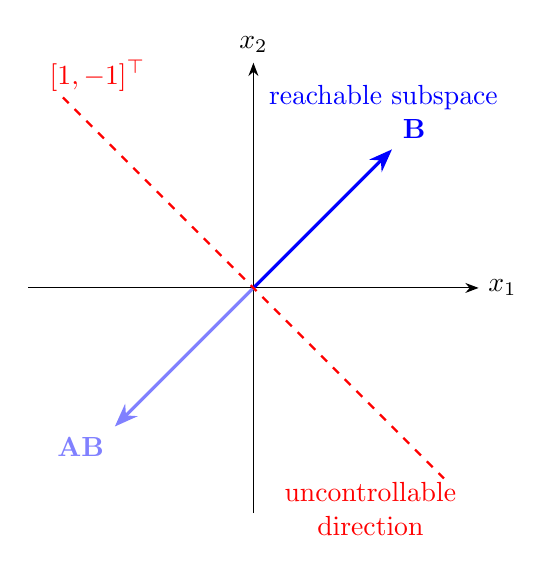
\begin{tikzpicture}[>=Stealth,scale=1.1]
  \draw[->] (-2.6,0)--(2.6,0) node[right] {$x_1$};
  \draw[->] (0,-2.6)--(0,2.6) node[above] {$x_2$};
  \draw[->,very thick,blue] (0,0)--(1.6,1.6) node[above right] {$\B$};
  \draw[->,very thick,blue!50] (0,0)--(-1.6,-1.6) node[below left] {$\A\B$};
  \draw[dashed,red,thick] (-2.2,2.2)--(2.2,-2.2);
  \node[red] at (-1.8,2.45) {$[1,-1]^\top$};
  \node[blue] at (1.5,2.2) {reachable subspace};
  \node[red,align=center] at (1.35,-2.55) {uncontrollable\\direction};
\end{tikzpicture}
\caption{Geometry of the $(A_2,B_2)$ example.  Both $B_2=[1,1]^\top$ and
$A_2B_2=B_2$ point along the diagonal, so only the diagonal is reachable.
The orthogonal direction $[1,-1]^\top$ is never affected by the input.  This
is why the controllability matrix has rank~1 even though the state space is
two-dimensional.}
\label{fig:controllability}
\end{figure}

\begin{recipe}[title={Testing controllability without guessing}]
\begin{enumerate}[leftmargin=1.4em,itemsep=2pt]
  \item Build $\C=[\B,\A\B,\dots,\A^{n-1}\B]$ and compute its rank.  Full rank
        means every state is reachable.
  \item If the rank is deficient, the left null space of $\C$ gives the
        unreachable directions (equivalently, use the PBH test
        $\operatorname{rank}[\A-\lambda I,\B]=n$ at each eigenvalue).
  \item Rank is binary; the singular values tell you how \emph{hard} each
        direction is to drive.  A full-rank system can still be very weakly
        controllable.
  \item Underactuation is a different question: compare the number of inputs
        with the number of degrees of freedom when the system is written as
        $\x=[q,\dot q]^\top$.  A system can be controllable and
        underactuated at the same time.
\end{enumerate}
\end{recipe}

\paragraph{Underactuation.}
$(\A_3,\B_3)$ has $x=[q,\dot q]^\top$ with a scalar $q$ and one input acting
directly on $\ddot q$: it is fully actuated.  $(\A_4,\B_4)$ has
$q=[x,\theta]^\top$ (two degrees of freedom) but only one input acting on
$\ddot x$; the angle $\theta$ has no actuator, so the system is
\emph{underactuated}.  This shows that controllability does not imply full
actuation: $(\A_4,\B_4)$ is controllable but underactuated.

%=====================================================================
\section{Section 3.8: Exercise 3.4}
%=====================================================================

\subsection{Model and linearisation}

For a pendulum with $m=l=1$, gravity $g=9.81$ and viscous damping
coefficient $b$,
\begin{equation}
\dot\theta=\omega,\qquad
\dot\omega=-g\sin\theta-b\omega,
\end{equation}
which corresponds to
$ml^2\ddot\theta+b\dot\theta+mgl\sin\theta=0$.  The equilibria are
$\x^\star=[0,0]^\top$ (down) and $[\pi,0]^\top$ (up).  The Jacobian is
\begin{equation}
A(\theta^\star)=
\begin{bmatrix}
0&1\\
-g\cos\theta^\star&-b
\end{bmatrix}.
\end{equation}

\begin{table}[H]
\centering
\caption{Eigenvalues of the Jacobian.}
\begin{tabular}{lcc}
\toprule
Condition & $\lambda_{1,2}$ & $\operatorname{sign}(\operatorname{Re}\lambda_{1,2})$ \\
\midrule
$b=0$, $\theta^\star=0$ & $\pm3.1321j$ & $0,0$ \\
$b=0$, $\theta^\star=\pi$ & $\pm3.1321$ & $+,-$ \\
$b=1$, $\theta^\star=0$ & $-0.5\pm3.0919j$ & $-,-$ \\
$b=1$, $\theta^\star=\pi$ & $2.6718,-3.6718$ & $+,-$ \\
\bottomrule
\end{tabular}
\end{table}

\begin{figure}[htbp]
\centering
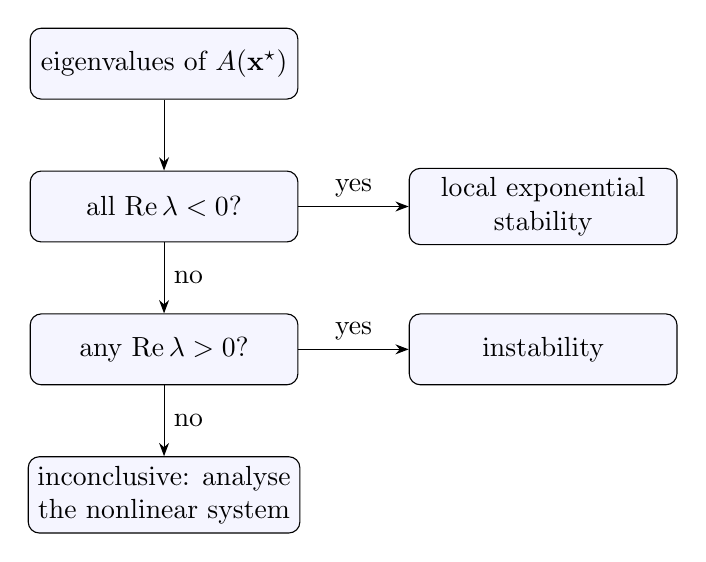
\begin{tikzpicture}[>=Stealth,node distance=0.9cm,
  box/.style={draw,rounded corners,align=center,fill=blue!4,
              minimum width=3.4cm,minimum height=0.9cm}]
  \node[box] (eig) {eigenvalues of $A(\x^\star)$};
  \node[box,below=of eig] (neg) {all $\operatorname{Re}\lambda<0$?};
  \node[box,below=of neg] (pos) {any $\operatorname{Re}\lambda>0$?};
  \node[box,right=1.4cm of neg] (stable) {local exponential\\stability};
  \node[box,right=1.4cm of pos] (unstable) {instability};
  \node[box,below=of pos] (inc) {inconclusive: analyse\\the nonlinear system};
  \draw[->] (eig)--(neg);
  \draw[->] (neg)--node[above] {yes}(stable);
  \draw[->] (neg)--node[right] {no}(pos);
  \draw[->] (pos)--node[above] {yes}(unstable);
  \draw[->] (pos)--node[right] {no}(inc);
\end{tikzpicture}
\caption{Decision diagram for the linearisation test.  The first two branches
are the standard Lyapunov indirect theorem.  The third branch
($\operatorname{Re}\lambda=0$) is the dangerous one: the linearisation alone
cannot decide, and one must go back to the nonlinear system.}
\label{fig:stability_flow}
\end{figure}

\begin{intuition}[title={The three stability words in plain language}]
\begin{itemize}[leftmargin=1.2em,itemsep=1pt]
  \item \textbf{Stable i.s.L.} (in the sense of Lyapunov): if you start close
        enough, you stay close.  You may oscillate forever.
  \item \textbf{Asymptotically stable}: you stay close \emph{and} you
        eventually converge to the equilibrium.
  \item \textbf{Exponentially stable}: you converge at least as fast as
        $e^{-ct}$ for some $c>0$.
\end{itemize}
For the undamped pendulum at the bottom, the energy is conserved: the
trajectory is a closed orbit.  It is stable i.s.L.\ but not asymptotically
stable, so it is certainly not exponentially stable.  For the damped
pendulum, the energy decreases and the trajectory spirals into the bottom:
all three properties hold (locally).  For the upright pendulum, a small
perturbation makes the pendulum fall: the equilibrium is a saddle and is
unstable.
\end{intuition}

\begin{pitfall}[title={Why $\operatorname{Re}\lambda=0$ needs care}]
At the undamped bottom, the eigenvalues are $\pm3.13j$: the real parts are
zero.  The linearised system is a centre, but the linearisation theorem is
inconclusive.  In this particular case the nonlinear system is also stable,
but that is a conclusion from the energy function, not from the eigenvalues.
A different nonlinear term with the same linearisation could be unstable.
This is why the exercise asks you to draw the phase portrait and to use the
nonlinear energy, not only the Jacobian.
\end{pitfall}

\subsection{Stability table}

\begin{table}[H]
\centering
\small
\caption{Stability of the nonlinear pendulum and its linearisation.  The
nonlinear entries are local properties; the exponential entry for the damped
hanging pendulum follows from the negative real parts of the linearisation.}
\begin{tabular}{lccccc}
\toprule
System & \shortstack{sign\\Re$\lambda_1$} & \shortstack{sign\\Re$\lambda_2$} & Stable i.s.L. & Asymp. stable & Exp. stable \\
\midrule
Nonlinear, $b=0$, $(0,0)$ & N/A & N/A & Yes & No & No \\
Nonlinear, $b=0$, $(\pi,0)$ & N/A & N/A & No & No & No \\
Linearization, $b=0$, $(0,0)$ & 0 & 0 & Yes & No & No \\
Linearization, $b=0$, $(\pi,0)$ & $+$ & $-$ & No & No & No \\
Nonlinear, $b=1$, $(0,0)$ & N/A & N/A & Yes & Yes & Yes \\
Nonlinear, $b=1$, $(\pi,0)$ & N/A & N/A & No & No & No \\
Linearization, $b=1$, $(0,0)$ & $-$ & $-$ & Yes & Yes & Yes \\
Linearization, $b=1$, $(\pi,0)$ & $+$ & $-$ & No & No & No \\
\bottomrule
\end{tabular}
\end{table}

\begin{figure}[htbp]
  \centering
  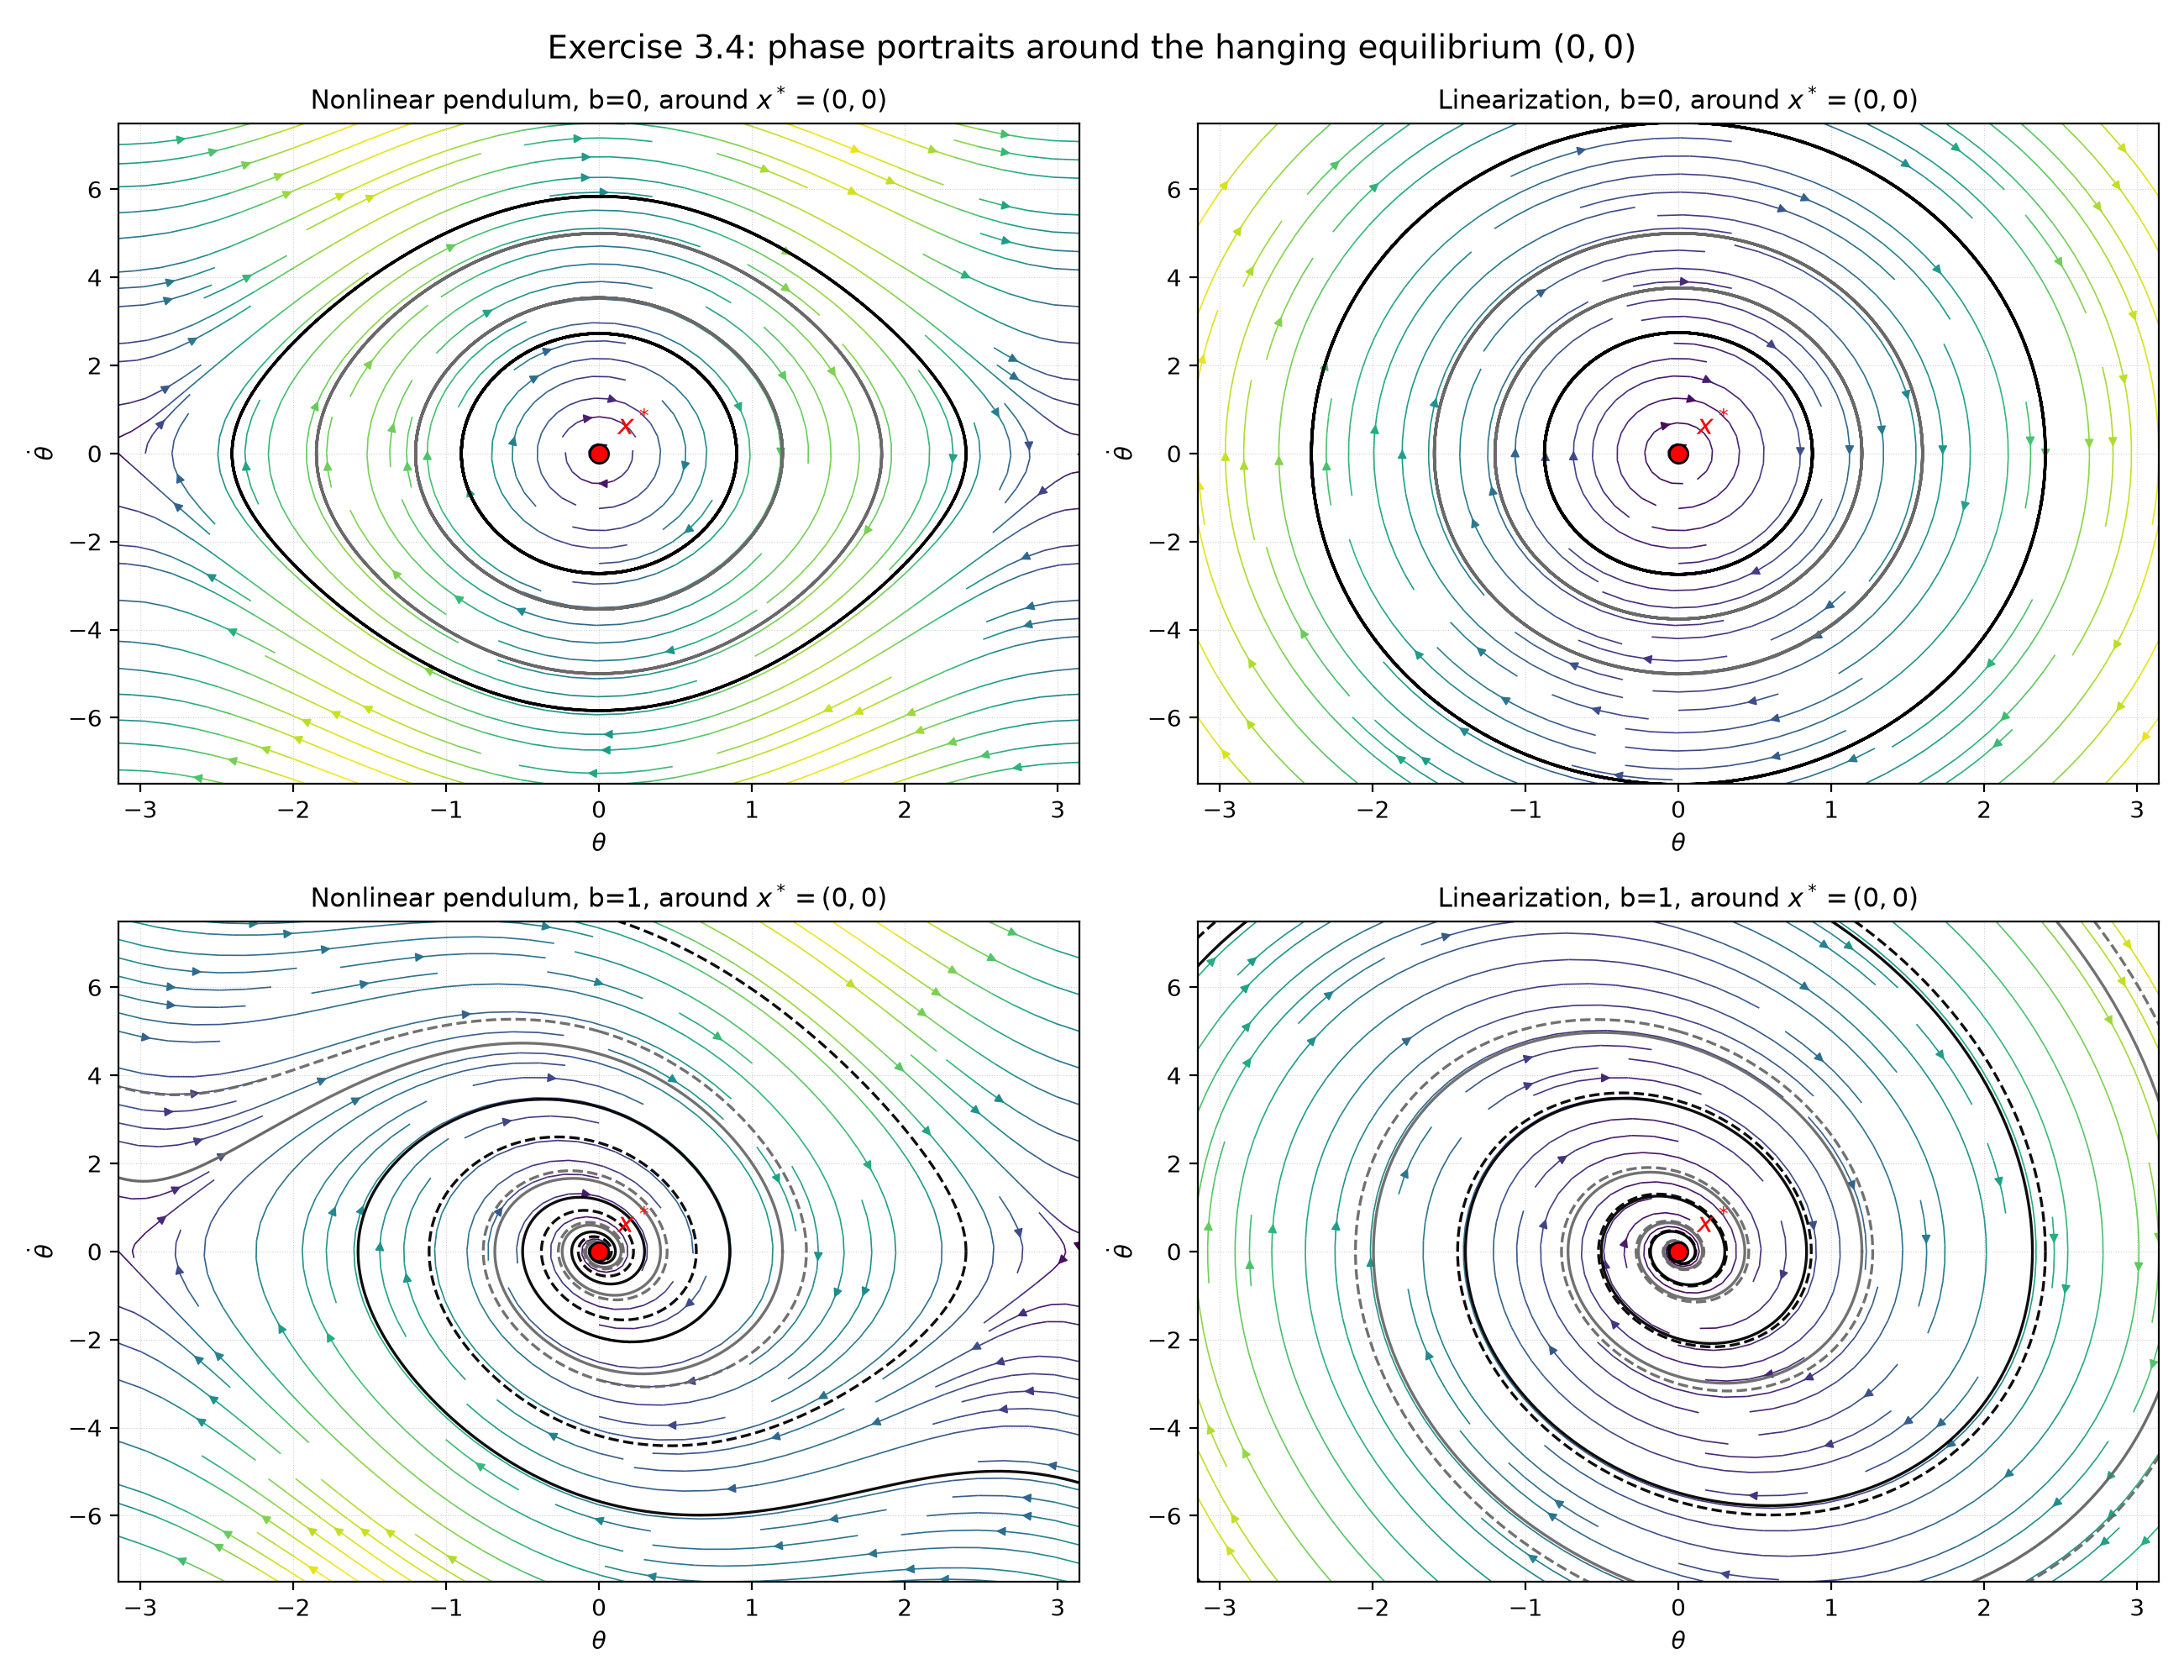
\includegraphics[width=0.92\textwidth]{s38_phase_down.png}
  \caption{Phase portraits around the hanging equilibrium $(0,0)$: nonlinear
  (left) and linearised (right), for $b=0$ (top) and $b=1$ (bottom).}
\end{figure}

\begin{figure}[htbp]
  \centering
  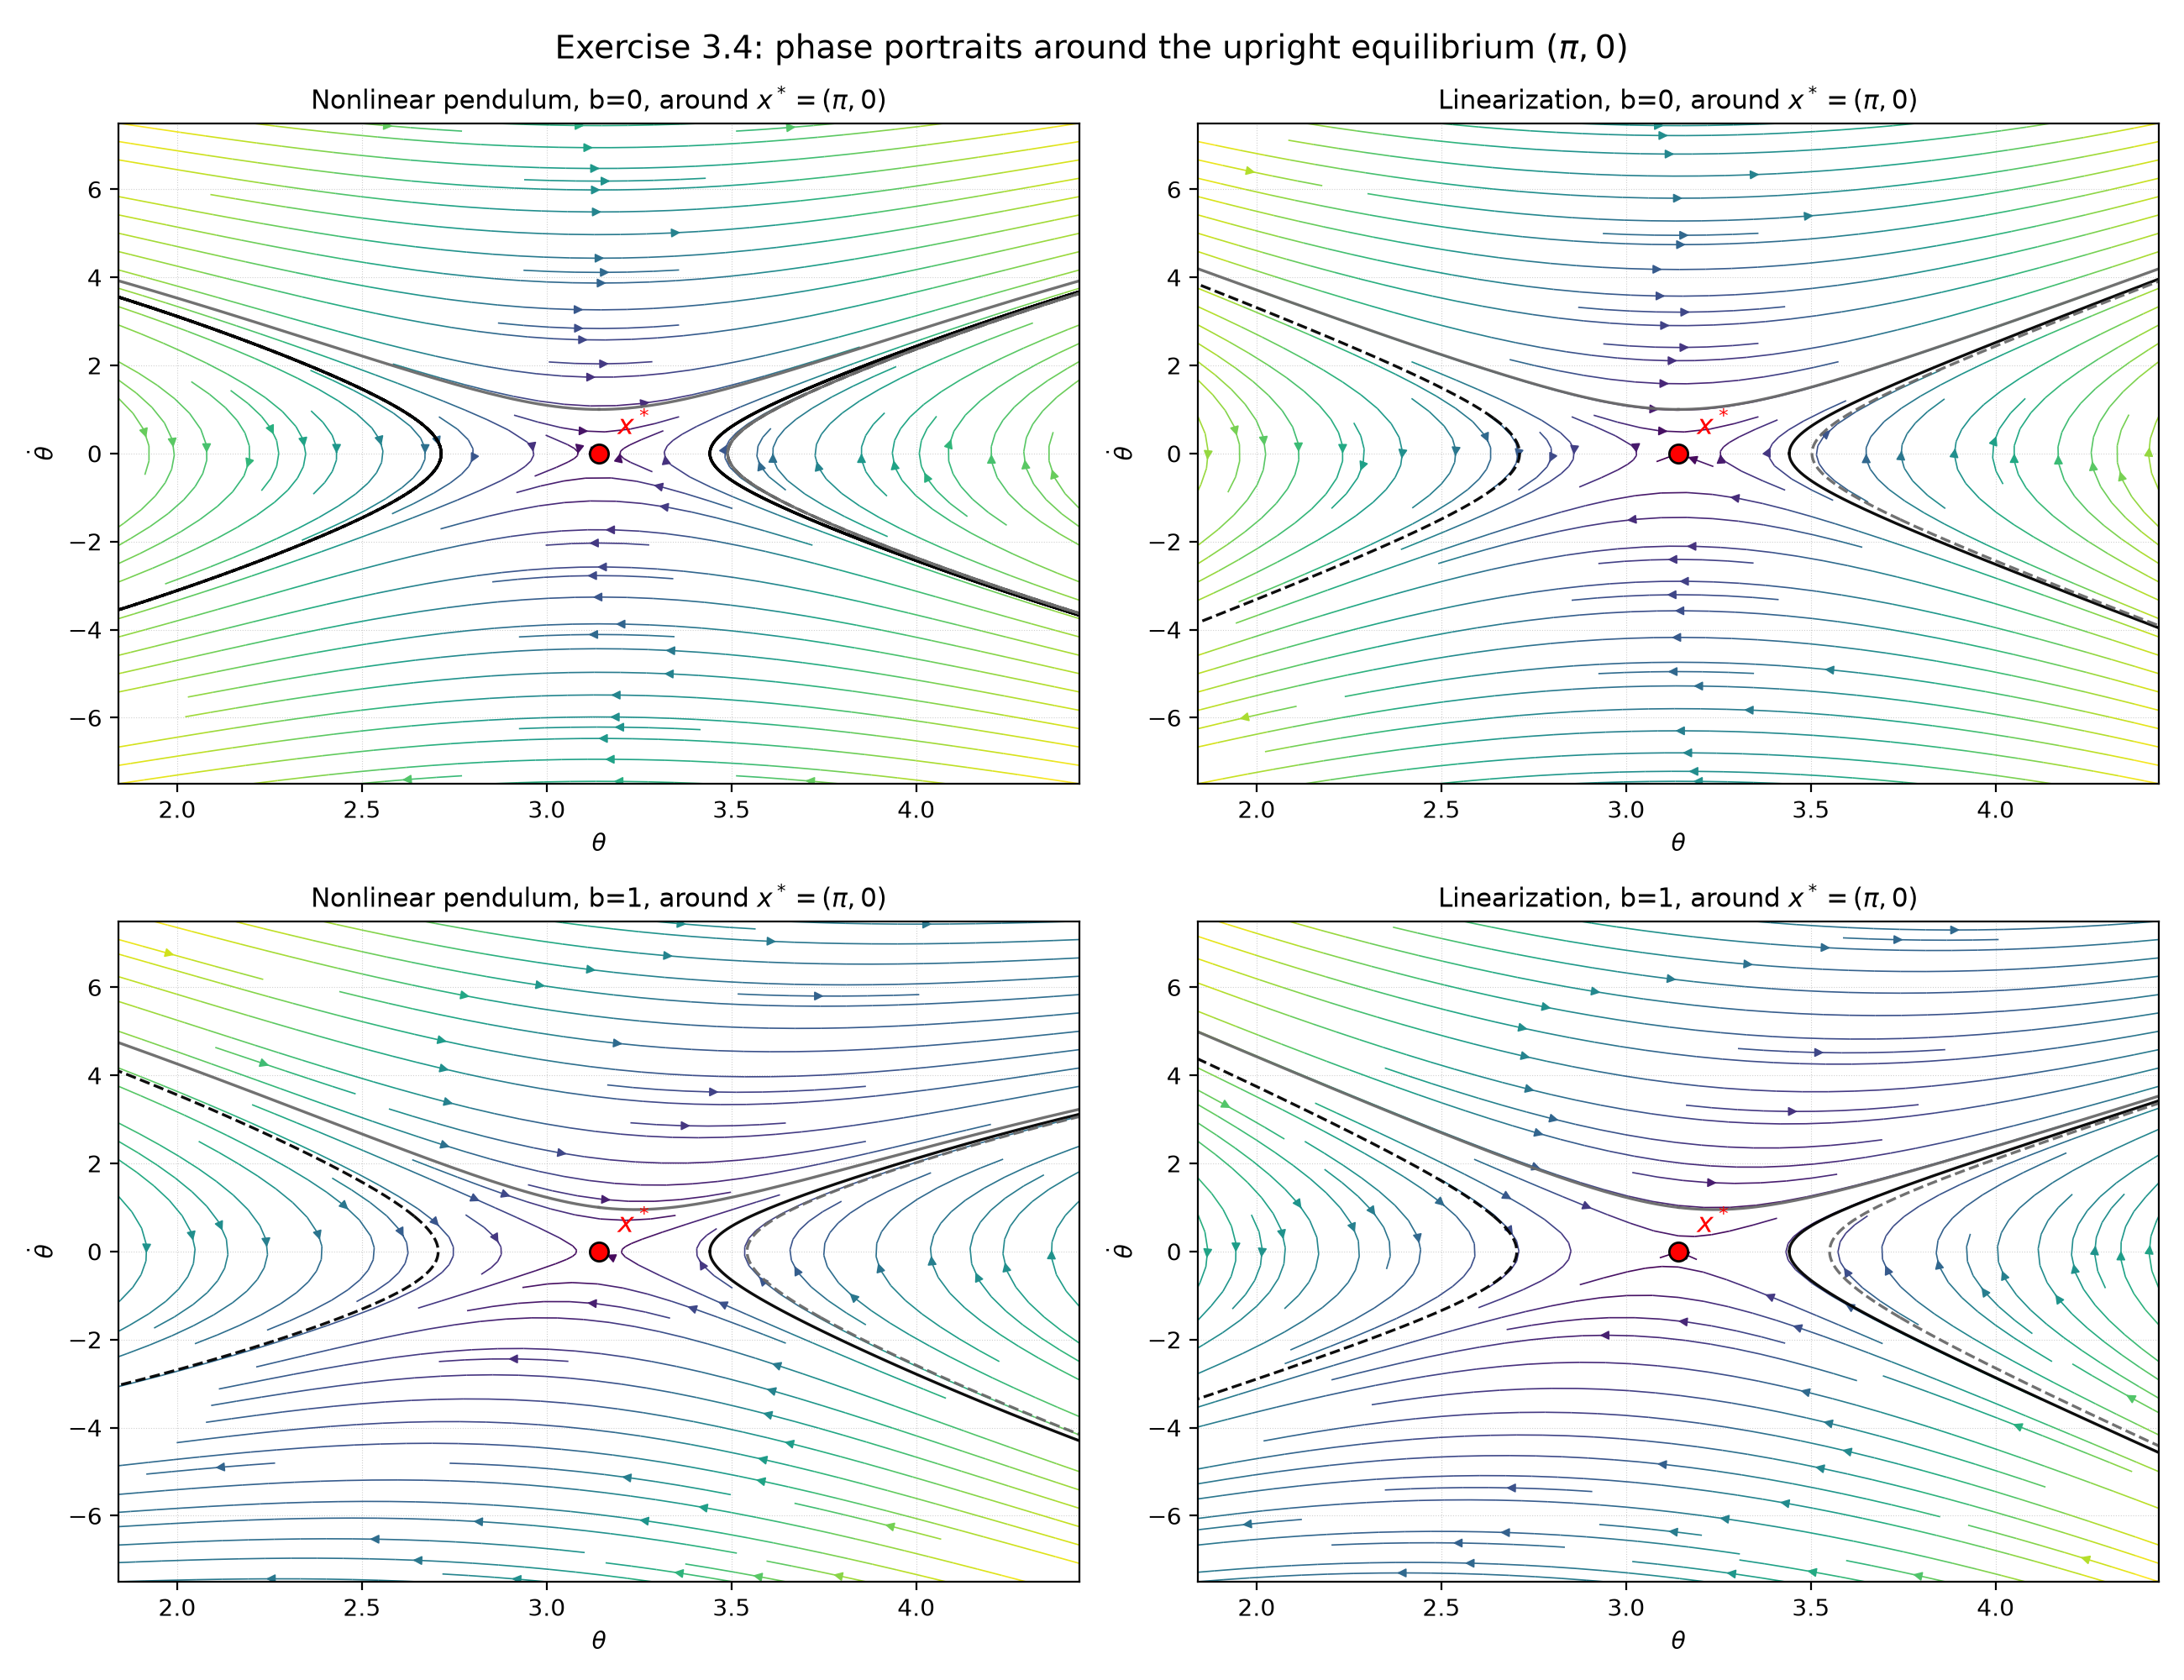
\includegraphics[width=0.92\textwidth]{s38_phase_up.png}
  \caption{Phase portraits around the upright equilibrium $(\pi,0)$:
  nonlinear (left) and linearised (right), for $b=0$ (top) and $b=1$
  (bottom).}
\end{figure}

\subsection{Discussion}

\begin{enumerate}[leftmargin=1.4em]
  \item For $b=0$ at $(0,0)$ the nonlinear system has closed orbits: it is
        stable i.s.L.\ but not asymptotically or exponentially stable.  The
        linearisation is a centre; when $\operatorname{Re}\lambda=0$ the
        linearisation theorem is inconclusive, and the nonlinear analysis
        (conserved energy) is required.
  \item At $(\pi,0)$ both the nonlinear system and its linearisation are
        unstable.  The phase portrait is a saddle; the stable manifold is a
        measure-zero set, so almost every perturbation falls.
  \item With $b=1$ at $(0,0)$ the eigenvalues have negative real parts and the
        nonlinear equilibrium is locally exponentially stable; the phase
        portrait spirals into the origin.
  \item With $b=1$ at $(\pi,0)$ one eigenvalue remains positive; damping does
        not stabilise the inverted pendulum.  Feedback is required.
  \item Linearisation determines local exponential stability when all
        eigenvalues have negative real parts, and instability when at least
        one has a positive real part.  It says nothing about global
        behaviour, finite escape times or the size of the basin of attraction.
\end{enumerate}

%=====================================================================
\section{Conclusions}
%=====================================================================

\begin{enumerate}[leftmargin=1.4em]
  \item \textbf{Underactuation vs.\ controllability.}  The acrobot and the
        cart-pole are underactuated, yet their linearisations are completely
        controllable.  Controllability is a rank property; the singular values
        and condition numbers reveal how hard the weakly controllable
        directions are to drive.
  \item \textbf{Local nature of linear control.}  LQR stabilises the
        linearisation and therefore gives local exponential stability.  The
        nonlinear simulations show finite basins of attraction.  Input
        saturation shrinks these basins substantially, especially for the
        acrobot with its $m_2$ sensitivity.
  \item \textbf{Non-minimum phase.}  Both the acrobot and the cart-pole have
        right-half-plane zeros.  State feedback cannot remove them; the closed
        loop exhibits undershoot, which is visible in the successful
        trajectories and explains part of the difficulty under saturation.
  \item \textbf{Quadrotor LQR.}  LQR works out of the box around a hover
        equilibrium with non-zero thrust.  The $Q/R$ trade-off and the absence
        of integral action (steady-state wind offset) are clearly visible in
        the planar study; the 3D model recovers from large attitude
        perturbations.
  \item \textbf{Section 3.8.}  The cart-pole linearisation is valid only near
        the upright point; the URDF single/double pendula were built and
        balanced (autograder 13/13 and 12/12); the discrete double integrator
        is reachable in two steps; only $(A_3,B_3)$ and $(A_4,B_4)$ of
        Exercise~3.3 are controllable, and $(A_4,B_4)$ is controllable but
        underactuated; the stability table of Exercise~3.4 separates the
        marginal, stable and unstable cases and highlights the limits of
        linearisation at zero real part.
\end{enumerate}

%=====================================================================
\section{Code and Reproduction}\label{sec:repro}
%=====================================================================

The complete code is provided in the repository.  The main entry points are:
\begin{center}
\small
\begin{tabular}{ll}
\toprule
Topic & Script / notebook \\
\midrule
Example 3.1 Acrobot & \texttt{exp1\_analysis/exp1\_analysis.py}, \texttt{Exp3'1-acrobot.ipynb} \\
Example 3.2 Cart-pole & \texttt{exp3\_2\_analysis/cp\_analysis.py}, \texttt{Exp3'2-cartpole.ipynb} \\
Example 3.5 LQR comparison & \texttt{exp3\_5\_analysis/lqr\_comparison.py}, \texttt{Exp3'5-LQR-analysis.ipynb} \\
Example 3.6 Quadrotor & \texttt{exp3\_6\_analysis/quadrotor\_analysis.py} \\
 & \texttt{Exp3'6-planar-quadrotor.ipynb}, \texttt{Exp3'6-quadrotor.ipynb} \\
Exercise 3.1 & \texttt{cartpole\_balancing.ipynb}, \texttt{ex3\_1\_balancing\_analysis.py} \\
Exercise 3.2 & \texttt{cartpoles\_urdf.ipynb}, \texttt{ex3\_2\_urdf\_lqr\_analysis.py} \\
Exercise 3.3 & \texttt{ex3\_3\_controllability.py} \\
Exercise 3.4 & \texttt{ex3\_4\_stability\_linearization.py} \\
\bottomrule
\end{tabular}
\end{center}

Commands (from the corresponding directories):
\begin{lstlisting}[language=bash]
/Users/leo/venvs/drake/bin/python exp1_analysis/exp1_analysis.py
/Users/leo/venvs/drake/bin/python exp3_2_analysis/cp_analysis.py
/Users/leo/venvs/drake/bin/python exp3_5_analysis/lqr_comparison.py
/Users/leo/venvs/drake/bin/python exp3_6_analysis/quadrotor_analysis.py
/Users/leo/venvs/drake/bin/python exercises_analysis/ex3_3_controllability.py
/Users/leo/venvs/drake/bin/python exercises_analysis/ex3_4_stability_linearization.py
\end{lstlisting}

The notebooks with autograders are executed headlessly with
\begin{lstlisting}[language=bash]
COLAB_TESTING=1 /Users/leo/venvs/drake/bin/jupyter nbconvert \
  --to notebook --execute --inplace --ExecutePreprocessor.timeout=180 \
  cartpoles_urdf.ipynb
\end{lstlisting}
\begin{sloppypar}
\texttt{COLAB\_TESTING=1} makes \texttt{running\_as\_notebook} false so that
\texttt{ModelVisualizer.Run(loop\_once=True)} does not block.
\end{sloppypar}

%=====================================================================
\appendix
\section{Key Code Snippets}
%=====================================================================

\subsection{Cart-pole linearisation and LQR}

\begin{lstlisting}[language=Python]
def f(x, u):
    c, s = np.cos(x[1]), np.sin(x[1])
    g = 9.81
    return np.array([
        x[2], x[3],
        (u[0] + s * (x[3]**2 + g * c)) / (1 + s**2),
        (-u[0] * c - x[3]**2 * c * s - 2 * g * s) / (1 + s**2)])

A = np.array([[0,0,1,0], [0,0,0,1],
              [0,9.81,0,0], [0,19.62,0,0]])
B = np.array([[0],[0],[1],[1]])
P = solve_continuous_are(A, B, Q, R)
K = np.linalg.solve(R, B.T @ P)
u = -K @ (x - x_star)
\end{lstlisting}

\subsection{URDF pendulum link and joint}

\begin{lstlisting}[language=XML]
<link name="pendulum0">
  <inertial>
    <origin xyz="0 0 -1" />
    <mass value="1" />
    <inertia ixx="0" ixy="0" ixz="0" iyy="0" iyz="0" izz="0" />
  </inertial>
  <visual>
    <origin xyz="0 0 -1" />
    <geometry><sphere radius="0.05" /></geometry>
  </visual>
  <visual>
    <origin xyz="0 0 -0.5" />
    <geometry><cylinder length="1" radius="0.01" /></geometry>
  </visual>
</link>
<joint name="theta0" type="continuous">
  <parent link="base" />
  <child link="pendulum0" />
  <origin xyz="0 0 0" />
  <axis xyz="0 -1 0" />
</joint>
\end{lstlisting}

\subsection{Controllability and two-step reachability}

\begin{lstlisting}[language=Python]
def controllability_matrix(A, B):
    n = A.shape[0]
    cols = [B]
    for _ in range(1, n):
        cols.append(A @ cols[-1])
    return np.hstack(cols)

def two_step_control(start, goal):
    i1, j1 = start
    i2, j2 = goal
    u0 = i2 - i1 - 2 * j1
    u1 = j2 - j1 - u0
    return (u0, u1)
\end{lstlisting}

\subsection{Quadrotor LQR}

\begin{lstlisting}[language=Python]
context = plant.CreateDefaultContext()
context.SetContinuousState(x_star)
u_hover = np.array([mass * gravity / 4.0] * 4)
plant.get_input_port(0).FixValue(context, u_hover)
Q = np.diag(np.concatenate(([10.0] * 6, [1.0] * 6)))
R = np.eye(4)
lqr = LinearQuadraticRegulator(plant, context, Q, R)
builder.Connect(lqr.get_output_port(0), plant.get_input_port(0))
builder.Connect(plant.get_output_port(0), lqr.get_input_port(0))
\end{lstlisting}

\end{document}
